% !Mode:: "TeX:UTF-8"
\def\usewhat{pdflatex}                              % 定义编译方式 dvipdfmx 或者 pdflatex ,默认为 dvipdfmx
                                                    % 方式编译,如果需要修改,只需改变花括号中的内容即可。
\documentclass[12pt,openright,twoside]{book}
\AtBeginDocument{\addtocontents{toc}{\protect\thispagestyle{only_foot}}} %强制目录页的第一页的页眉页脚样式

% !Mode:: "TeX:UTF-8"
%  Authors: 张井   Jing Zhang: prayever@gmail.com     天津大学2010级管理与经济学部信息管理与信息系统专业硕士生
%           余蓝涛 Lantao Yu: lantaoyu1991@gmail.com  天津大学2008级精密仪器与光电子工程学院测控技术与仪器专业本科生

%%%%%%%%%% Package %%%%%%%%%%%%

\usepackage{graphicx}                       % 支持插图处理
%\usepackage[a4paper,text={150true mm,224true mm},top=35.5true mm,left=30true mm,head=5true mm,headsep=2.5true mm,foot=8.5true mm]{geometry}
%\usepackage[a4paper,text={153true mm,243true mm},top= 25true mm,left=31.8 true mm,head=6true mm,headsep=6true mm,foot=16.5true mm]{geometry}
\usepackage[a4paper,top=27.5mm,bottom=25.4mm,left=35.7mm,right=27.7mm,head=6true mm,headsep=6true mm,foot=7.9true mm]{geometry}

                                            % 支持版面尺寸设置
\usepackage{titlesec}                       % 控制标题的宏包
\usepackage{titletoc}                       % 控制目录的宏包
\usepackage{fancyhdr}                       % fancyhdr宏包 支持页眉和页脚的相关定义
\usepackage[UTF8]{ctex}                     % 支持中文显示
\usepackage{color}                          % 支持彩色
\usepackage{amsmath}                        % AMSLaTeX宏包 用来排出更加漂亮的公式
\usepackage{amssymb}                        % 数学符号生成命令
\usepackage[below]{placeins}                %允许上一个section的浮动图形出现在下一个section的开始部分,还提供\FloatBarrier命令,使所有未处理的浮动图形立即被处理
\usepackage{flafter}                        % 使得所有浮动体不能被放置在其浮动环境之前,以免浮动体在引述它的文本之前出现.
\usepackage{multirow}                       % 使用Multirow宏包,使得表格可以合并多个row格
\usepackage{booktabs}                       % 表格,横的粗线;\specialrule{1pt}{0pt}{0pt}
\usepackage{longtable}                      % 支持跨页的表格。
\usepackage{tabularx}                       % 自动设置表格的列宽
\usepackage{subfigure}                      % 支持子图 %centerlast 设置最后一行是否居中
\usepackage[subfigure]{ccaption}            % 支持子图的中文标题
\usepackage[sort&compress,numbers]{natbib}  % 支持引用缩写的宏包
\usepackage{enumitem}                       % 使用enumitem宏包,改变列表项的格式
\usepackage{calc}                           % 长度可以用+ - * / 进行计算
\usepackage{txfonts}                        % 字体宏包
\usepackage{bm}                             % 处理数学公式中的黑斜体的宏包
\usepackage[amsmath,thmmarks,hyperref]{ntheorem}  % 定理类环境宏包,其中 amsmath 选项用来兼容 AMS LaTeX 的宏包
\usepackage{CJKnumb}                        % 提供将阿拉伯数字转换成中文数字的命令
\usepackage{indentfirst}                    % 首行缩进宏包
\usepackage{CJKutf8}                        % 用在UTF8编码环境下,它可以自动调用CJK,同时针对UTF8编码作了设置。
\usepackage{algorithm}                      % bigben:算法
\usepackage{algpseudocode}
%\usepackage{hypbmsec}                      % 用来控制书签中标题显示内容

%\usepackage{pdflatex}
%如果您的pdf制作中文书签有乱码使用如下命令,就可以解决了
\usepackage[pdflatex, unicode,               % pdflatex, pdftex 这里决定运行文件的方式不同
            pdfstartview=FitH,
            %CJKbookmarks=true,
            bookmarksnumbered=true,
            bookmarksopen=true,
            colorlinks=false,
            pdfborder={0 0 1},
            citecolor=blue,
            linkcolor=red,
            anchorcolor=green,
            urlcolor=blue,
            breaklinks=true
            ]{hyperref}
\usepackage{mathrsfs}

                      % 定义本文所使用宏包
\graphicspath{{figures/}}                  % 定义所有的.eps 文件在figures 子目录下
\begin{document}                           % 开始全文
\begin{CJK*}{UTF8}{song}                   % 开始中文字体使用
% !Mode:: "TeX:UTF-8"
%  Authors: 张井   Jing Zhang: prayever@gmail.com     天津大学2010级管理与经济学部信息管理与信息系统专业硕士生
%           余蓝涛 Lantao Yu: lantaoyu1991@gmail.com  天津大学2008级精密仪器与光电子工程学院测控技术与仪器专业本科生

%%%%%%%%%% Fonts Definition and Basics %%%%%%%%%%%%%%%%%
\newcommand{\song}{\CJKfamily{song}}    % 宋体
\newcommand{\fs}{\CJKfamily{fs}}        % 仿宋体
\newcommand{\kai}{\CJKfamily{kai}}      % 楷体
\newcommand{\hei}{\CJKfamily{hei}}      % 黑体
\newcommand{\li}{\CJKfamily{li}}        % 隶书
\newcommand{\yihao}{\fontsize{26pt}{26pt}\selectfont}       % 一号, 1.倍行距
\newcommand{\xiaoyi}{\fontsize{24pt}{24pt}\selectfont}      % 小一, 1.倍行距
\newcommand{\erhao}{\fontsize{22pt}{1.25\baselineskip}\selectfont}       % 二号, 1.25倍行距
\newcommand{\xiaoer}{\fontsize{18pt}{18pt}\selectfont}      % 小二, 单倍行距
\newcommand{\sanhao}{\fontsize{16pt}{16pt}\selectfont}      % 三号, 1.倍行距
\newcommand{\xiaosan}{\fontsize{15pt}{15pt}\selectfont}     % 小三, 1.倍行距
\newcommand{\sihao}{\fontsize{14pt}{14pt}\selectfont}       % 四号, 1.0倍行距
\newcommand{\xiaosi}{\fontsize{12pt}{20pt}\selectfont}      % 小四, 1.倍行距
\newcommand{\wuhao}{\fontsize{10.5pt}{10.5pt}\selectfont}   % 五号, 单倍行距
\newcommand{\xiaowu}{\fontsize{9pt}{9pt}\selectfont}        % 小五, 单倍行距

%\CJKcaption{gb_452}
\CJKtilde  % 重新定义了波浪符~的意义
\newcommand\prechaptername{第}
\newcommand\postchaptername{章}

% 调整罗列环境的布局
\setitemize{leftmargin=3em,itemsep=0em,partopsep=0em,parsep=0em,topsep=-0em}
\setenumerate{leftmargin=3em,itemsep=0em,partopsep=0em,parsep=0em,topsep=0em}
%\setlength{\baselineskip}{20pt}
%\renewcommand{\baselinestretch}{1.38} % 设置行距

%避免宏包 hyperref 和 arydshln 不兼容带来的目录链接失效的问题。
\def\temp{\relax}
\let\temp\addcontentsline
\gdef\addcontentsline{\phantomsection\temp}

% 自定义项目列表标签及格式 \begin{publist} 列表项 \end{publist}
\newcounter{pubctr} %自定义新计数器
\newenvironment{publist}{%%%%%定义新环境
\begin{list}{[\arabic{pubctr}]} %%标签格式
    {
     \usecounter{pubctr}
     \setlength{\leftmargin}{2.5em}     % 左边界 \leftmargin =\itemindent + \labelwidth + \labelsep
     \setlength{\itemindent}{0em}     % 标号缩进量
     \setlength{\labelsep}{1em}       % 标号和列表项之间的距离,默认0.5em
     \setlength{\rightmargin}{0em}    % 右边界
     \setlength{\topsep}{0ex}         % 列表到上下文的垂直距离
     \setlength{\parsep}{0ex}         % 段落间距
     \setlength{\itemsep}{0ex}        % 标签间距
     \setlength{\listparindent}{0pt} % 段落缩进量
    }}
{\end{list}}%%%%%

\makeatletter
\renewcommand\normalsize{
  \@setfontsize\normalsize{12pt}{12pt} % 小四对应12pt
  \setlength\abovedisplayskip{4pt}
  \setlength\abovedisplayshortskip{4pt}
  \setlength\belowdisplayskip{\abovedisplayskip}
  \setlength\belowdisplayshortskip{\abovedisplayshortskip}
  \setlength{\baselineskip}{20pt} % 设置固定行间距为20pt
  \let\@listi\@listI}
\def\defaultfont{\renewcommand{\baselinestretch}{1.0}\normalsize\selectfont}
% 设置行距和段落间垂直距离
\renewcommand{\CJKglue}{\hskip -0.08pt plus 0.08\baselineskip} % 每行大概35个字符

\makeatother
%%%%%%%%%%%%% Contents %%%%%%%%%%%%%%%%% 目录样式修改,(天津大学关于博士、硕士学位论文统一格式的规定 2016.10.24)

\renewcommand{\contentsname}{目\qquad录}
\setcounter{tocdepth}{2}
\titlecontents{chapter}[0em]{\vspace{0pt}\xiaosi\song\bfseries}%
             {\prechaptername\thecontentslabel\postchaptername\quad}{} %
             {\hspace{.5em}\titlerule*[7pt]{.}\xiaosi\contentspage}
\titlecontents{section}[2em]{\vspace{0pt}\xiaosi\song} %
            {\thecontentslabel\quad}{} %
            {\hspace{.5em}\titlerule*[7pt]{.}\xiaosi\contentspage}
\titlecontents{subsection}[4em]{\vspace{0pt}\xiaosi\song} %
            {\thecontentslabel\quad}{} %
            {\hspace{.5em}\titlerule*[7pt]{.}\xiaosi\contentspage}
%\titlecontents{subsubsection}[6em]{\vspace{0pt}\xiaosi\song} %
%            {\thecontentslabel\quad}{} %
%            {\hspace{.5em}\titlerule*[7pt]{.}\xiaosi\contentspage}

%%%%%%%%%% Chapter and Section %%%%%%%%%%%%%%%%% 各级标题样式((天津大学关于博士、硕士学位论文统一格式的规定 2016.10.24))
\setcounter{secnumdepth}{4}
\setlength{\parindent}{2em}
\renewcommand{\chaptername}{\prechaptername\thechapter\postchaptername}
\titleformat{\chapter}{\centering\xiaosan\hei}{\chaptername}{1em}{}
\titlespacing{\chapter}{0pt}{33pt}{33pt}
\titleformat{\section}{\sihao\hei}{\thesection}{1em}{}
\titlespacing{\section}{0pt}{21pt}{21pt}
\titleformat{\subsection}{\sihao\hei}{\thesubsection}{1em}{}
\titlespacing{\subsection}{0pt}{13pt}{13pt}
\titleformat{\subsubsection}{\xiaosi\hei}{\thesubsubsection}{1em}{}
\titlespacing{\subsubsection}{0pt}{10pt}{10pt}

%%%%%%%%%% Table, Figure and Equation %%%%%%%%%%%%%%%%%
\renewcommand{\tablename}{表} % 插表题头
\renewcommand{\figurename}{图} % 插图题头
\renewcommand{\thefigure}{\arabic{chapter}-\arabic{figure}} % 使图编号为 7-1 的格式 %\protect{~}
\renewcommand{\thetable}{\arabic{chapter}-\arabic{table}}%使表编号为 7-1 的格式
\renewcommand{\theequation}{\arabic{chapter}-\arabic{equation}}%使公式编号为 7-1 的格式
\renewcommand{\thesubfigure}{(\alph{subfigure})}%使子图编号为 (a)的格式
\renewcommand{\thesubtable}{(\alph{subtable})} %使子表编号为 (a)的格式
\makeatletter
\renewcommand{\p@subfigure}{\thefigure~} %使子图引用为 7-1 a) 的格式,母图编号和子图编号之间用~加一个空格
\makeatother


%% 定制浮动图形和表格标题样式
\makeatletter
\long\def\@makecaption#1#2{%
   \vskip\abovecaptionskip
   \sbox\@tempboxa{\centering\wuhao\song{#1\qquad #2} }%
   \ifdim \wd\@tempboxa >\hsize
     \centering\wuhao\song{#1\qquad #2} \par
   \else
     \global \@minipagefalse
     \hb@xt@\hsize{\hfil\box\@tempboxa\hfil}%
   \fi
   \vskip\belowcaptionskip}
\makeatother
\captiondelim{~~~~} %用来控制longtable表头分隔符

%%%%%%%%%% Theorem Environment %%%%%%%%%%%%%%%%%
\theoremstyle{plain}
\theorembodyfont{\song\rmfamily}
\theoremheaderfont{\hei\rmfamily}
\newtheorem{theorem}{定理~}[chapter]
\newtheorem{lemma}{引理~}[chapter]
\newtheorem{axiom}{公理~}[chapter]
\newtheorem{proposition}{命题~}[chapter]
\newtheorem{corollary}{推论~}[chapter]
\newtheorem{definition}{定义~}[chapter]
\newtheorem{conjecture}{猜想~}[chapter]
\newtheorem{example}{例~}[chapter]
\newtheorem{remark}{注~}[chapter]
%\newtheorem{algorithm}{算法~}[chapter]
\newenvironment{proof}{\noindent{\hei 证明:}}{\hfill $ \square $ \vskip 4mm}
\theoremsymbol{$\square$}

%%%%%%%%%% Page: number, header and footer  %%%%%%%%%%%%%%%%%

%\frontmatter 或 \pagenumbering{roman}
%\mainmatter 或 \pagenumbering{arabic}
\makeatletter
\renewcommand\frontmatter{\clearpage
  \@mainmatterfalse
  \pagenumbering{Roman}} % 正文前罗马字体编号
\makeatother


%%%%%%%%%% References %%%%%%%%%%%%%%%%%
\renewcommand{\bibname}{参考文献}
% 重定义参考文献样式,来自thu
\makeatletter
\renewenvironment{thebibliography}[1]{%
   \chapter*{\bibname}%
   \xiaosi
   \list{\@biblabel{\@arabic\c@enumiv}}%
        {\renewcommand{\makelabel}[1]{##1\hfill}
         \setlength{\baselineskip}{17pt}
         \settowidth\labelwidth{0.5cm}
         \setlength{\labelsep}{0pt}
         \setlength{\itemindent}{0pt}
         \setlength{\leftmargin}{\labelwidth+\labelsep}
         \addtolength{\itemsep}{-0.7em}
         \usecounter{enumiv}%
         \let\p@enumiv\@empty
         \renewcommand\theenumiv{\@arabic\c@enumiv}}%
    \sloppy\frenchspacing
    \clubpenalty4000%
    \@clubpenalty \clubpenalty
    \widowpenalty4000%
    \interlinepenalty4000%
    \sfcode`\.\@m}
   {\def\@noitemerr
     {\@latex@warning{Empty `thebibliography' environment}}%
    \endlist\frenchspacing}
\makeatother

\addtolength{\bibsep}{3pt} % 增加参考文献间的垂直间距
\setlength{\bibhang}{2em} %每个条目自第二行起缩进的距离

% 参考文献引用作为上标出现
%\newcommand{\citeup}[1]{\textsuperscript{\cite{#1}}}
\makeatletter
    \def\@cite#1#2{\textsuperscript{[{#1\if@tempswa , #2\fi}]}}
\makeatother
%% 引用格式
\bibpunct{[}{]}{,}{s}{}{,}

%%%%%%%%%% Cover %%%%%%%%%%%%%%%%%
% 封面、摘要、版权、致谢格式定义
\makeatletter
\def\ctitle#1{\def\@ctitle{#1}}\def\@ctitle{}
\def\etitle#1{\def\@etitle{#1}}\def\@etitle{}
\def\caffil#1{\def\@caffil{#1}}\def\@caffil{}
\def\cmacrosubject#1{\def\@cmacrosubject{#1}}\def\@cmacrosubject{}
\def\cmacrosubjecttitle#1{\def\@cmacrosubjecttitle{#1}}\def\@cmacrosubjecttitle{}
\def\csubject#1{\def\@csubject{#1}}\def\@csubject{}
\def\csubjecttitle#1{\def\@csubjecttitle{#1}}\def\@csubjecttitle{}
\def\cgrade#1{\def\@cgrade{#1}}\def\@cgrade{}
\def\cauthor#1{\def\@cauthor{#1}}\def\@cauthor{}
\def\cauthortitle#1{\def\@cauthortitle{#1}}\def\@cauthortitle{}
\def\csupervisor#1{\def\@csupervisor{#1}}\def\@csupervisor{}
\def\csupervisortitle#1{\def\@csupervisortitle{#1}}\def\@csupervisortitle{}
\def\ccorsupervisor#1{\def\@ccorsupervisor{#1}}\def\@ccorsupervisor{}
\def\ccorsupervisortitle#1{\def\@ccorsupervisortitle{#1}}\def\@ccorsupervisortitle{}
\def\cdate#1{\def\@cdate{#1}}\def\@cdate{}
\def\declaretitle#1{\def\@declaretitle{#1}}\def\@declaretitle{}
\def\declarecontent#1{\def\@declarecontent{#1}}\def\@declarecontent{}
\def\authorizationtitle#1{\def\@authorizationtitle{#1}}\def\@authorizationtitle{}
\def\authorizationcontent#1{\def\@authorizationcontent{#1}}\def\@authorizationconent{}
\def\authorizationadd#1{\def\@authorizationadd{#1}}\def\@authorizationadd{}
\def\authorsigncap#1{\def\@authorsigncap{#1}}\def\@authorsigncap{}
\def\supervisorsigncap#1{\def\@supervisorsigncap{#1}}\def\@supervisorsigncap{}
\def\signdatecap#1{\def\@signdatecap{#1}}\def\@signdatecap{}
\long\def\cabstract#1{\long\def\@cabstract{#1}}\long\def\@cabstract{}
\long\def\eabstract#1{\long\def\@eabstract{#1}}\long\def\@eabstract{}
\def\ckeywords#1{\def\@ckeywords{#1}}\def\@ckeywords{}
\def\ekeywords#1{\def\@ekeywords{#1}}\def\@ekeywords{}

%在book文件类别下,\leftmark自动存录各章之章名,\rightmark记录节标题
\pagestyle{fancy}
%去掉章节标题中的数字 务必放到\pagestyle{fancy}之后才会起作用
%%不要注销这一行,否则页眉会变成:“第1章1  绪论”样式
\renewcommand{\chaptermark}[1]{\markboth{\chaptername~\ #1}{}}
  \fancyhf{}
  \fancyhead[C]{\song\wuhao \leftmark} % 页眉显示章节名称
  %\fancyhead[CO]{\song\wuhao \@cheading}
  %\fancyhead[CE]{\song\wuhao \@cheading}
  \fancyfoot[C]{\song\xiaowu ~\thepage~}
  \renewcommand{\headrulewidth}{0.7pt}%
  \renewcommand{\footrulewidth}{0pt}%

\fancypagestyle{plain}{% 设置开章页页眉页脚风格
    \fancyhf{}%
    \fancyhead[C]{\song\wuhao \leftmark}
    \fancyfoot[C]{\song\xiaowu ~\thepage~ } %%首页页脚格式
    \renewcommand{\headrulewidth}{0.7pt}%
    \renewcommand{\footrulewidth}{0pt}%
}

\fancypagestyle{only_foot}{% 设置摘要、目录的页眉页脚风格:无页眉((天津大学关于博士、硕士学位论文统一格式的规定 2016.10.24)貌似要这种only_foot的样式)
    \fancyhf{}%
    \fancyfoot[C]{\song\xiaowu ~\thepage~ }
    \renewcommand{\headrulewidth}{0pt}%
    \renewcommand{\footrulewidth}{0pt}%
}


\newlength{\@title@width}
\def\@put@covertitle#1{\makebox[\@title@width][s]{#1}}
% 定义封面
\def\makecover{
\clearpage{\pagestyle{empty}\cleardoublepage}
   \phantomsection
    \pdfbookmark[-1]{\@ctitle}{ctitle}

    \begin{titlepage}
      \vspace*{0.8cm}
      \begin{center}

      \vspace*{1cm}
      \begin{center}
      \renewcommand{\baselinestretch}{1.25} % 设置行距
      \song\erhao\textbf{\@ctitle} % 修改成宋体加粗 (天津大学关于博士、硕士学位论文统一格式的规定, 2016.10.24)
      \renewcommand{\baselinestretch}{1.25} % 设置行距
      \end{center}
      \vspace*{1cm}

      \vspace*{1cm}

      \begin{center}
      \renewcommand{\baselinestretch}{1.25} % 设置行距
      \song\erhao\textbf{\@etitle}  % 修改成宋体加粗1.25倍行距(英文默认变成了Times new Roman) (天津大学关于博士、硕士学位论文统一格式的规定, 2016.10.24)
      \renewcommand{\baselinestretch}{1.25} % 设置行距
      \end{center}

      \vspace*{3cm}
      \setlength{\@title@width}{5em}
      {\song\sihao
      \begin{tabular}{p{\@title@width}@{:}l}
        \@put@covertitle{\@csubjecttitle} & \@csubject \\
        \@put@covertitle{\@cauthortitle} & \@cauthor \\
        \@put@covertitle{\@csupervisortitle} & \@csupervisor \\
        \@put@covertitle{\@ccorsupervisortitle} & \@ccorsupervisor \\
      \end{tabular}
      }

  \vspace*{5cm}
  \song\sihao\@caffil \\
  \song\sihao\@cdate

\end{center}
%  另起一页: 独创性声明和学位论文版权使用授权书
\newpage
    \clearpage{\pagestyle{empty}\cleardoublepage} %去除空白页的页眉页脚(由于每章从奇数页开始因此有空白页)
    \thispagestyle{empty} %去掉页眉页脚
    \vspace*{1cm}
    \renewcommand{\baselinestretch}{1} % 设置行距
    \begin{center}\song\xiaoer{\@declaretitle}\end{center}\par
    \vspace*{0.5cm}
    \song\xiaosi{\@declarecontent}\par
    \vspace*{1cm}
    {\song\xiaosi
    \@authorsigncap \makebox[2.5cm][s]{}
    \@signdatecap \makebox[2cm][s]{} 年 \makebox[1cm][s]{} 月 \makebox[1cm][s]{} 日
    }

    \vspace*{3cm}
    \begin{center}\song\xiaoer{\@authorizationtitle}\end{center}\par
    \vspace*{1cm}
    {
    \song\xiaosi{\@authorizationcontent}

    \@authorizationadd\par
    }

    \vspace*{2cm}
    {\song\xiaosi\setlength{\parindent}{-0.45em}
    \begin{tabularx}{\textwidth}{ll}
        \@authorsigncap \makebox[3.5cm][s]{}  & \@supervisorsigncap \makebox[3.5cm][s]{}   \\
         &  \\
        \@signdatecap \makebox[1.5cm][s]{} 年 \makebox[1cm][s]{} 月 \makebox[1cm][s]{} 日 &
         \@signdatecap \makebox[1.5cm][s]{} 年 \makebox[1cm][s]{} 月 \makebox[1cm][s]{} 日 \\
    \end{tabularx}
    }
\end{titlepage}

%%%%%%%%%%%%%%%%%%%   Abstract and Keywords  %%%%%%%%%%%%%%%%%%%%%%%
\clearpage{\pagestyle{empty}\cleardoublepage} %去除空白页的页眉页脚(由于每章从奇数页开始因此有空白页)
\markboth{摘~要}{摘~要}
\addcontentsline{toc}{chapter}{摘\qquad 要}
\chapter*{\centering\song\erhao\textbf{摘\qquad 要}}
\thispagestyle{only_foot}

\setcounter{page}{1}
\song\defaultfont
\@cabstract
%\vspace{\baselineskip}

%\hangafter=1\hangindent=52.3pt\noindent   %如果取消该行注释,关键词换行时将会自动缩进
\noindent
{\hei\sihao 关键词:} \@ckeywords

%%%%%%%%%%%%%%%%%%%   English Abstract  %%%%%%%%%%%%%%%%%%%%%%%%%%%%%%
\clearpage{\pagestyle{empty}\cleardoublepage} %去除空白页的页眉页脚(由于每章从奇数页开始因此有空白页)
\markboth{ABSTRACT}{ABSTRACT}
\addcontentsline{toc}{chapter}{ABSTRACT}
\chapter*{\centering\erhao\textbf{ABSTRACT}}
\thispagestyle{only_foot}
%\vspace{\baselineskip}
\@eabstract
%\vspace{\baselineskip}

%\hangafter=1\hangindent=60pt\noindent  %如果取消该行注释,KEY WORDS换行时将会自动缩进
\noindent
{\sihao\textbf{KEY WORDS:}}  \@ekeywords
}

\makeatother
                       % 完成对论文各个部分格式的设置
\frontmatter                               % 以下是论文导言部分,包括论文的封面,中英文摘要和中文目录
% !Mode:: "TeX:UTF-8"


\ctitle{基于深度学习的超像素分割和图像分割}  %封面用论文标题,自己可手动断行
\etitle{A Study on Indoor Localization Based on fingerprinting and inertial measurements}
%\etitle{A Study on Subspace Clustering Algorithm \\for High-dimensional Data}
\caffil{天津大学智能与计算学部} %学院名称
\csubjecttitle{工程领域}
\csubject{软件工程}   %专业
\cauthortitle{作者姓名}     % 学位
\cauthor{***}   %学生姓名
\csupervisortitle{指导教师}
\csupervisor{***~~教授} %导师姓名
\ccorsupervisortitle{企业导师}
\ccorsupervisor{***}

\declaretitle{独创性声明}
\declarecontent{
本人声明所呈交的学位论文是本人在导师指导下进行的研究工作和取得的研究成果,除了文中特别加以标注和致谢之处外,论文中不包含其他人已经发表或撰写过的研究成果,也不包含为获得 {\underline{\kai\sihao\textbf{~~天津大学~~}}} 或其他教育机构的学位或证书而使用过的材料。与我一同工作的同志对本研究所做的任何贡献均已在论文中作了明确的说明并表示了谢意。
}
\authorizationtitle{学位论文版权使用授权书}
\authorizationcontent{
本学位论文作者完全了解{\underline{\kai\sihao\textbf{~~天津大学~~}}}有关保留、使用学位论文的规定。特授权{\underline{\kai\sihao\textbf{~~天津大学~~}}} 可以将学位论文的全部或部分内容编入有关数据库进行检索,并采用影印、缩印或扫描等复制手段保存、汇编以供查阅和借阅。同意学校向国家有关部门或机构送交论文的复印件和磁盘。
}
\authorizationadd{(保密的学位论文在解密后适用本授权说明)}
\authorsigncap{学位论文作者签名:}
\supervisorsigncap{导师签名:}
\signdatecap{签字日期:}


\cdate{\CJKdigits{\the\year} 年\CJKnumber{\the\month} 月 \CJKnumber{\the\day} 日}
% 如需改成二零一二年四月二十五日的格式,可以直接输入,即如下所示
\cdate{二零一六年十月}
% \cdate{\the\year 年\the\month 月 \the\day 日} % 此日期显示格式为阿拉伯数字 如2012年4月25日
\cabstract{

图像分割和超像素生成已经被研究很多年,但仍然是计算机视觉中一个重要的课题。
虽然很多先进的计算机视觉的算法已经被用于图像分割和超像素生成方面,
但是没有端到端可训练的算法来实现同时产生超像素和图像分割。
对此,我们提出了一个端到端的可训练网络,它可以同时产生超像素和进行图像分割。
我们的网络架构如图3-1所示。我们使用完全卷积网络和迭代可微聚类算法来获得超像素。
接下来,我们采用超像素池层来获得超像素特征,并以此计算相邻超像素之间的相似度。
如果相似度大于预先设定的阈值,则通过简单的步骤将其合并,得到目标片段。
我们使用BSDS500数据集训练网络,并将我们的结果与最先进的结果进行比较,并得到了很好的结果。

本文提出的网络具有以下特点:
\begin{itemize}
\item 我们的网络是端到端可训练的,可以很容易地组装成其他深层网络结构,以备后续应用。
\item 我们的网络可以产生超像素并得到分割结果,这是更有效的。与现有算法相比,该算法具有优良的性能和更高的精度。
\end{itemize}
}

\ckeywords{图像分割,超像素,深度学习}

\eabstract{

Image segmentation and superpixel generation have been studied for many years, 
and they are still active research topics in computer vision. 
Although many advanced computer vision algorithms have been used for image segmentation and superpixel generation, 
there is no end-to-end trainable algorithm that generates superpixels and segment images simultaneously. 
Specifically, we propose an end-to-end trainable network 
which can generate superpixels and perform image segmentation simultaneously.
The architecture of our network is shown in Fig. 3-1. 
We use a fully convolutional network and the iterative differentiable clustering algorithm to obtain superpixels. 
Next, we adopt the superpixel pooling layer to get the superpixel features, 
with which the similarity between adjacent superpixels can be calculated. 
If the similarity is greater than the preset threshold, 
we merge them according to a simple procedure to get object segments. 
We train the network using BSDS500 segmentation benchmark dataset, 
compare our result with state-of-the-art ones and get good results.

The proposed network has the following characteristics:
\begin{itemize}
\item Our network is end-to-end trainable and can be easily as sembled into other deep network structures for subsequent applications.
\item Our network can generate superpixels and get segmentation results, which is more efficient. The proposed algorithm has excellent performance and has higher precision than existing algorithms.
\end{itemize}

}

\ekeywords{Image segmentation, Superpixel, Deep learning}

\makecover
\clearpage
                      % 封面 摘要

%%%%%%%%%%   目录   %%%%%%%%%%
\clearpage{\pagestyle{empty}\cleardoublepage}
\defaultfont
\clearpage{
    \pagestyle{only_foot}
    \tableofcontents                           % 中文目录
    \thispagestyle{only_foot}
}
\clearpage{\pagestyle{empty}\cleardoublepage}

%%%%%%%%%% 正文部分内容  %%%%%%%%%%
\mainmatter\defaultfont\sloppy\raggedbottom
%% !Mode:: "TeX:UTF-8"

\chapter{模板介绍与注意事项}
\section{模板说明}

TJUThesis~是为了帮助天津大学毕业生撰写毕业论文而编写的~\LaTeX~论文模板,其前提是用户已经能处理一般的~\LaTeX~文档,并对~BibTeX~有一定了解,如果你从来没有接触过~\LaTeX~,建议先学习相关基础知识,磨刀不误砍柴工,能有助你更好使用模板。

由于个人水平有限,虽然现在的这个版本基本上满足了学校的要求,但难免存在不足之处,欢迎大家积极反馈,更希望天津大学~\LaTeX~爱好者能一同完善此模板,让更多同学受益。

如有模板的疑问或有意向加入模板的维护和编写队伍中来,请给作者: prayever@gmail.com(张井),lantaoyu1991@gmail.com(余蓝涛)写信。

\section{下载安装}
TJUThesis~主页:~\url{http://tjuthesis.googlecode.com/}。除此之外,不再维护任何镜像。

\section{目录内容}
本~\LaTeX{}~模板的源文件即为研究生毕业设计论文中使用的模板,用户可以通过修改这些文件来编辑自己的毕业论文。
\begin{itemize}
\item{tjumain.tex}:主文件,包含封面部分和其他章节的引用信息。
\item{preface}: 包含本科毕业设计论文的封面和中英文摘要。
\item{body}: 包含本文正文中的所有章节。
\begin{itemize}
\item{intros.tex}: 包括本~\LaTeX{}~模板的介绍,编译方法和使用方法。
\item{figures.tex}: 包含论文中图片的插入和引用方法。
\item{tables.tex}: 包含论文中表格的插入和引用方法。
\item{equations.tex}: 包含论文中数学符号、公式的书写和排版方法。
\item{others.tex}: 包含论文中使用的罗列环境,定理环境等其他环境的排版方法。
\item{conclusion.tex}: 包含本文的总结。
\end{itemize}
\item{setup}:存放论文所使用的宏包和全文格式的定义。
\item{appendix}:存放作者的发表论文和参加科研情况说明以及致谢文件。
\item{references/reference.bib}:存放论文所引用的全部参考文献信息。
\item{clean.bat}:双击此文件,可以用来清理~tjumain.tex~在编译之后生成的所有附属文件,如后缀名为~.aux~,~.log~,~.bak~的文件。
\end{itemize}

需要说明的是,以上文件名并不是固定的,各位同学可以新建一个~tex~文件,例如~algorithm.tex,放在~body~目录下,并且在~tjumain.tex~中调用:
\begin{verbatim}
    \include{body/algorithm.tex}
\end{verbatim}
来引用之。当然你也可以重命名这些文件,只要~include~中的文件名是存在且合法,~\LaTeX~总能找到这些文件的。

在你写作某一章节的时候,你可能需要随时预览排版效果并~Debug,这时你可以在其他章节的\verb|\include|命令前加上一个\%,这代表注释掉本行,例如:
\begin{verbatim}
%%%%%%%%%%%%%%%%%%%%%%%%%%%%%%%%
           正文部分
%%%%%%%%%%%%%%%%%%%%%%%%%%%%%%%%
\mainmatter
% !Mode:: "TeX:UTF-8"

\chapter{模板介绍与注意事项}
\section{模板说明}

TJUThesis~是为了帮助天津大学毕业生撰写毕业论文而编写的~\LaTeX~论文模板,其前提是用户已经能处理一般的~\LaTeX~文档,并对~BibTeX~有一定了解,如果你从来没有接触过~\LaTeX~,建议先学习相关基础知识,磨刀不误砍柴工,能有助你更好使用模板。

由于个人水平有限,虽然现在的这个版本基本上满足了学校的要求,但难免存在不足之处,欢迎大家积极反馈,更希望天津大学~\LaTeX~爱好者能一同完善此模板,让更多同学受益。

如有模板的疑问或有意向加入模板的维护和编写队伍中来,请给作者: prayever@gmail.com(张井),lantaoyu1991@gmail.com(余蓝涛)写信。

\section{下载安装}
TJUThesis~主页:~\url{http://tjuthesis.googlecode.com/}。除此之外,不再维护任何镜像。

\section{目录内容}
本~\LaTeX{}~模板的源文件即为研究生毕业设计论文中使用的模板,用户可以通过修改这些文件来编辑自己的毕业论文。
\begin{itemize}
\item{tjumain.tex}:主文件,包含封面部分和其他章节的引用信息。
\item{preface}: 包含本科毕业设计论文的封面和中英文摘要。
\item{body}: 包含本文正文中的所有章节。
\begin{itemize}
\item{intros.tex}: 包括本~\LaTeX{}~模板的介绍,编译方法和使用方法。
\item{figures.tex}: 包含论文中图片的插入和引用方法。
\item{tables.tex}: 包含论文中表格的插入和引用方法。
\item{equations.tex}: 包含论文中数学符号、公式的书写和排版方法。
\item{others.tex}: 包含论文中使用的罗列环境,定理环境等其他环境的排版方法。
\item{conclusion.tex}: 包含本文的总结。
\end{itemize}
\item{setup}:存放论文所使用的宏包和全文格式的定义。
\item{appendix}:存放作者的发表论文和参加科研情况说明以及致谢文件。
\item{references/reference.bib}:存放论文所引用的全部参考文献信息。
\item{clean.bat}:双击此文件,可以用来清理~tjumain.tex~在编译之后生成的所有附属文件,如后缀名为~.aux~,~.log~,~.bak~的文件。
\end{itemize}

需要说明的是,以上文件名并不是固定的,各位同学可以新建一个~tex~文件,例如~algorithm.tex,放在~body~目录下,并且在~tjumain.tex~中调用:
\begin{verbatim}
    \include{body/algorithm.tex}
\end{verbatim}
来引用之。当然你也可以重命名这些文件,只要~include~中的文件名是存在且合法,~\LaTeX~总能找到这些文件的。

在你写作某一章节的时候,你可能需要随时预览排版效果并~Debug,这时你可以在其他章节的\verb|\include|命令前加上一个\%,这代表注释掉本行,例如:
\begin{verbatim}
%%%%%%%%%%%%%%%%%%%%%%%%%%%%%%%%
           正文部分
%%%%%%%%%%%%%%%%%%%%%%%%%%%%%%%%
\mainmatter
% !Mode:: "TeX:UTF-8"

\chapter{模板介绍与注意事项}
\section{模板说明}

TJUThesis~是为了帮助天津大学毕业生撰写毕业论文而编写的~\LaTeX~论文模板,其前提是用户已经能处理一般的~\LaTeX~文档,并对~BibTeX~有一定了解,如果你从来没有接触过~\LaTeX~,建议先学习相关基础知识,磨刀不误砍柴工,能有助你更好使用模板。

由于个人水平有限,虽然现在的这个版本基本上满足了学校的要求,但难免存在不足之处,欢迎大家积极反馈,更希望天津大学~\LaTeX~爱好者能一同完善此模板,让更多同学受益。

如有模板的疑问或有意向加入模板的维护和编写队伍中来,请给作者: prayever@gmail.com(张井),lantaoyu1991@gmail.com(余蓝涛)写信。

\section{下载安装}
TJUThesis~主页:~\url{http://tjuthesis.googlecode.com/}。除此之外,不再维护任何镜像。

\section{目录内容}
本~\LaTeX{}~模板的源文件即为研究生毕业设计论文中使用的模板,用户可以通过修改这些文件来编辑自己的毕业论文。
\begin{itemize}
\item{tjumain.tex}:主文件,包含封面部分和其他章节的引用信息。
\item{preface}: 包含本科毕业设计论文的封面和中英文摘要。
\item{body}: 包含本文正文中的所有章节。
\begin{itemize}
\item{intros.tex}: 包括本~\LaTeX{}~模板的介绍,编译方法和使用方法。
\item{figures.tex}: 包含论文中图片的插入和引用方法。
\item{tables.tex}: 包含论文中表格的插入和引用方法。
\item{equations.tex}: 包含论文中数学符号、公式的书写和排版方法。
\item{others.tex}: 包含论文中使用的罗列环境,定理环境等其他环境的排版方法。
\item{conclusion.tex}: 包含本文的总结。
\end{itemize}
\item{setup}:存放论文所使用的宏包和全文格式的定义。
\item{appendix}:存放作者的发表论文和参加科研情况说明以及致谢文件。
\item{references/reference.bib}:存放论文所引用的全部参考文献信息。
\item{clean.bat}:双击此文件,可以用来清理~tjumain.tex~在编译之后生成的所有附属文件,如后缀名为~.aux~,~.log~,~.bak~的文件。
\end{itemize}

需要说明的是,以上文件名并不是固定的,各位同学可以新建一个~tex~文件,例如~algorithm.tex,放在~body~目录下,并且在~tjumain.tex~中调用:
\begin{verbatim}
    \include{body/algorithm.tex}
\end{verbatim}
来引用之。当然你也可以重命名这些文件,只要~include~中的文件名是存在且合法,~\LaTeX~总能找到这些文件的。

在你写作某一章节的时候,你可能需要随时预览排版效果并~Debug,这时你可以在其他章节的\verb|\include|命令前加上一个\%,这代表注释掉本行,例如:
\begin{verbatim}
%%%%%%%%%%%%%%%%%%%%%%%%%%%%%%%%
           正文部分
%%%%%%%%%%%%%%%%%%%%%%%%%%%%%%%%
\mainmatter
\include{body/intros}
%%\include{body/figures}
%%\include{body/tables}
%%\include{body/equations}
%%\include{body/others}
%%\include{body/conclusion}
\end{verbatim}
那么,编译的时候就只编译未加~\%~的一章,在这个例子中,即本章~intros。

理论上,并不一定要把每章放在不同的文件中。但是这种自顶向下,分章节写作、编译的方法有利于提高效率,大大减少~Debug~过程中的编译时间,同时减小风险。

\section{参考文献生成方法}

\LaTeX~具有插入参考文献的能力。Google Scholar~网站上存在兼容~BibTeX~的参考文献信息,通过以下几个步骤,可以轻松完成参考文献的生成。
\begin{itemize}
  \item 在\href{http://scholar.google.com/}{谷歌学术搜索}中,
        点击\href{http://scholar.google.com/scholar_preferences?hl=en&as_sdt=0,5}{学术搜索设置}。
  \item 页面打开之后,在\textbf{文献管理软件}选项中选择\textbf{显示导入~BibTeX~的链接},单击保存设置,退出。
  \item 在谷歌学术搜索中检索到文献后,在文献条目区域单击导入~BibTeX~选项,页面中出现文献的引用信息。
  \item 将文献引用信息的内容复制之后,添加到~references~文件夹下的~reference.bib~中。
\end{itemize}

\section{编译注意事项}
\begin{enumerate}
  \item 由于模板使用~UTF-8~编码,所以源文件应该保存成~UTF-8~格式,否则可能出现中文字符无法识别的错误。
  本模板中每一个~.tex~文件的文件的开头已经加上一行:\\
    \verb|% !Mode:: "TeX:UTF-8"|\\
     这样可以确保~.tex~文件默认使用~UTF-8~的格式打开。读者如果删去此行,很有可能会导致中文字符显示乱码。
     在~WinEdt~编辑器中可以使用以下两种方式保存成~UTF-8~格式:
      \begin{enumerate}
        \item 先建立~.tex~文件,另存为~.tex~文件时,选择用~UTF-8~格式保存。
        \item
            在~WinEdt~编辑器中,选择\\
            \mbox{~Document$\to$Document Settings$\to$Document Mode $\to$TeX:UTF-8} 同时在~WinEdt~最下面的状态栏中,可以看到该文档是~TeX~格式还是~TeX:UTF-8~格式。
            当文档为~TeX:UTF-8~格式时,状态栏一般显示:
            \makebox[\textwidth][l]{Wrap | Indent | INS | LINE |Spell | TeX:UTF-8 | -src~等。}
      \end{enumerate}
  \item 如果在pdf书签中,中文显示乱码的话,则注意以下说明:
    \begin{verbatim}
        \usepackage{CJKutf8}
        % 1. 如果使用CJKutf8
        %    Hyperref中应使用unicode参数
        % 2. 如果使用CJK
        %    Hyperref则使用CJKbookmarks参数
        %    可惜得到的PDF书签是乱码,建议弃用
        % 3. Unicode选项和CJKbookmarks不能同时使用
        \usepackage[
        %CJKbookmarks=true,
        unicode=true
        ]{hyperref}
     \end{verbatim}
 \item 建议采用以下两种编译方式:
  \begin{enumerate}
     \item latex + bibtex + latex + latex + dvi2pdf. 在这种编译情况下,对应的~tjumain.tex~文件的第一行是\verb|\def\usewhat{dvipdfmx}|~(缺省设置)。 此时,所有图片文件应该保存为~.eps~格式,如~figures~文件夹里~.eps~图片。
          如果您选择在命令行中操作,可以在编译的时候依次输入~latex tjumain, bibtex tjumain, latex tjumain, latex tjumain~和~dvipdfmx tjumain, 编译完成之后,需要手动打开~pdf~文件。
     \item pdflatex + pdflatex. 在这种编译情况下,对应的~tjumain.tex~文件的第一行应该改为\verb|\def\usewhat{pdflatex}|~。 此时, 编译不支持~.eps~图片格式,此时需要在命令行下使用~epstopdf~指令将~figures~文件夹下 的~.eps~文件转化成~.pdf~文件格式,命令行中操作格式为~epstopdf a.eps~。
          在命令行编译的时候,依次输入~pdflatex tjumain~和~pdflatex tjumain, 编译完成之后,需要手动打开~pdf~文件。
  \end{enumerate}
\end{enumerate}

\section{系统要求}
    CTEX 2.8, MiKTeX 2.8, TeX Live 2009~或以上版本。使用推荐的~WinEdt 6.0~编辑器,可以完成文件的编辑和编译工作。

\section{\TeX~简介}

以下内容是~milksea@bbs.ctex.org~撰写的关于~\TeX~的简单介绍,略有改动。
注意这不是一个入门教程,不讲~\TeX~系统的配置安装,也不讲具体的~\LaTeX~代码。
这里仅仅试图以一些只言片语来解释:
进入这个门槛之前新手应该知道的注意事项,以及遇到问题以后该去如何解决问题。

\subsection{什么是 \TeX/\LaTeX,我是否应该选择它~?}

\TeX~是最早由高德纳(Donald Knuth)教授创建的一门标记式宏语言,
用来排版科技文章,尤其擅长处理复杂的数学公式。\TeX~同时也是处理这一语言的排版软件。
\LaTeX~是 Leslie Lamport 在~\TeX~基础上按内容/格式分离和模块化等思想建立的一集~\TeX~上的格式。

\TeX~本身的领域是专业排版领域
但现在~TeX/LaTeX~也被广泛用于生成电子文档甚至幻灯片等,~\TeX~语言的数学部分
偶尔也在其他一些地方使用。但注意~\TeX~并不适用于文书处理(Microsoft Office 的领域,以前和现在都不是)。

选择使用~\TeX/\LaTeX~的理由包括:
\begin{itemize}
\item 免费软件;
\item 专业的排版效果;
\item 是事实上的专业数学排版标准;
\item 广泛的西文期刊接收甚或只接收 LaTeX 格式的投稿;
\item[] ……
\end{itemize}
不选择使用~\TeX/\LaTeX~的理由包括:
\begin{itemize}
\item 需要相当精力学习;
\item 图文混合排版能力不够强;
\item 仅在数学、物理、计算机等领域流行;
\item 中文期刊的支持较差;
\item[] ……
\end{itemize}

请尽量清醒看待网上经常见到的关于~\TeX~与其他软件的优劣比较和口水战。在选择使用或离开之前,请先考虑
\TeX~的应用领域,想想它是否适合你的需要。


\subsection{我该用什么编辑器~?}

编辑器功能有简有繁,特色不一,从简单的纯文本编辑器到繁复的 Emacs,因人而易。基本功能有语法高亮、方便编译预览就很好了,扩充功能和定制有无限的可能。初学者可以使用功能简单、使用方便的专用编辑器,如 ~TeXWorks、Kile、WinEdt~等,或者类似所见即所得功能的~LyX;熟悉的人可以使用定制性更强的~Notepad++、SciTE、Vim、Emacs ~等。这方面的介绍很多,一开始不妨多试几种,找到最适合自己的才是最好的。

另外提醒一句,编辑器只是工作的助手,不必把它看得太重。

\subsection{我应该看什么~\LaTeX~读物~?}

这不是一个容易回答的问题,因为有许多选择,也同样有许多不合适的选择。
这里只是选出一个比较好的答案。更多更详细的介绍可以在版面和网上寻找(注意时效)。

近两年~\TeX~的中文处理发展很快,目前没有哪本书在中文处理方面给出一个最新进展的合适综述,
因而下面的介绍也不主要考虑中文处理。

\begin{enumerate}

\item 我能阅读英文。
\begin{enumerate}
\item 迅速入门:ltxprimer.pdf (LaTeX Tutorials: A Primer, India TUG)
\item 系统学习:A Guide to LaTeX, 4th Edition, Addison-Wesley
               有机械工业出版社的影印版(《\LaTeX{}~实用教程》)
\item 深入学习:要读许多书和文档,TeXbook 是必读的
\item 细节学习:去读你使用的每一个宏包的说明文档
\item 专题学习:阅读讲数学公式、图形、表格、字体等的专题文档
\end{enumerate}

\item 我更愿意阅读中文。
\begin{enumerate}
\item 迅速入门:lnotes.pdf (LaTeX Notes, 1.20, Alpha Huang)
\item 系统学习:《\LaTeXe{}~科技排版指南》,邓建松(电子版)
      如果不好找,可以阅读《\LaTeXe~入门与提高》第二版,陈志杰等,或者 《\LaTeXe~完全学习手册》,胡伟
\item 深入学习:~TeXbook0.pdf~(特可爱原本,TeXbook 的中译,xianxian)
\item 具体问题释疑:~CTeX-FAQ.pdf~,\\
        吴凌云,~\url{http://www.ctex.org/CTeXFAQ}~
\end{enumerate}
\end{enumerate}

遇见问题和解决问题的过程可以快速提高自己的技能,建议此时:
\begin{itemize}
  \item 利用~Google~搜索。
  \item 清楚,扼要地提出你的问题。
\end{itemize}

\subsection{什么知识会过时~?什么不会~?}

\TeX~是排版语言,也是广泛使用的软件,并且不断在发展中;
因此,总有一些东西会很快过时。作为学习~\TeX~的人,
免不了要看各种各样的书籍、电子文档和网络论坛上的只言片语,
因此了解什么知识会迅速过时,什么知识不会是十分重要的。

最稳定的是关于~Primitive \TeX~和~Plain \TeX~的知识,也就是 Knuth
在他的《The TeXbook》中介绍的内容。因为~\TeX~
系统开发的初衷就是稳定性,要求今天的文档到很久以后仍可以得到完全相同的结果,
因此 Knuth 限定了他的~\TeX~语言和相关实现的命令、语法。这些内容许多年来就没有多少变化,
在未来的一些年里也不会有什么变化。
Primitive \TeX~和 Plain \TeX~的知识主要包括 \TeX~排版的基本算法和原理,
盒子的原理,底层的 \TeX~命令等。其中技巧性的东西大多在宏包设计中,
初学者一般不会接触到很多;而基本原理则是常常被提到的,
譬如,~\TeX~把一切排版内容作为盒子(box)处理。

相对稳定的是关于基本~\LaTeXe~
的知识,也包括围绕~\LaTeXe~的一些核心宏包的知识。~\LaTeXe~
是自~1993~年以来的一个稳定的~\LaTeX~版本,直到最近的一次修订
(2005 年)都没有大的变动。
\LaTeX~的下一个计划中的版本~\LaTeX 3~遥遥无期,在可预见的将来,~\LaTeXe~不会过时。
\LaTeXe~的知识是目前大部分~\LaTeX~书籍的主体内容。关于~\LaTeX~的标准文档类
~(article、report、book、letter、slide~等),关于基本数学公式的输入,
文档的章节层次,表格和矩阵,图表浮动体,LR 盒子与段落盒子……
这些~\LaTeX~的核心内容都是最常用的,相对稳定的。
与~\LaTeXe~相匹配的核心宏包,
如~graphics(x)、ifthen、fontenc、doc~等,也同样是相对稳定的。
还有一些被非常广泛应用的宏包,如~amsmath~系列,也可以看作是相对稳定的。

简单地说,关于基本~\TeX/\LaTeX~的语言,都是比较稳定的。与之对应,实现或者支持~\TeX/\LaTeX~语言的软件,
包括在~\TeX/\LaTeX~基础上建立的新的宏,都不大稳定。

容易过时的是关于第三方~\LaTeX~宏包的知识、第三方~\TeX~工具的知识,以及新兴~\TeX~相关软件的知识等。
~\TeX~和~\LaTeX~语言是追求稳定的;但无论是宏包还是工具,作为不断更新软件,它们是不稳定的。
容易过时的技术很多,而且现在广泛地出现在几乎所有~\LaTeX~文档之中,因此需要特别引起注意:
宏包的过时的原因可能是宏包本身的升级换代带来了新功能或不兼容,
也可能是同一功能的更新更好的宏包代替了旧的宏包。前者的典型例子比如绘图宏包~PGF/TikZ~,
现在的~2.00~版功能十分强大,和旧的~1.1x~版相差很大,和更旧的~0.x~版本则几乎完全不同;后
者的典型例子比如~caption~宏包先是被更新的~caption2~宏包代替,后来~caption~宏包更新又使得
caption2 宏包完全过时。——安装更新的发行版可以避免使用过旧的宏包;
认真阅读宏包自带的文档而不是搜索得到的陈旧片断可以避免采用过时的代码。

工具过时的主要原因也是升级换代和被其他工具替换。前者的典型例子是编辑器
WinEdt~在~5.5~以后的版本支持~UTF-8~编码,而旧版本不支持;
后者的典型例子是中文字体安装工具从~GBKFonts~到~xGBKFonts~到~FontsGen~不断被取代。
图形插入是一个在~\TeX~实现、宏包与外围工具方面都更新很快的东西。
在过去,最常用的输出格式是~PS(PostScript)~格式,因此插入的图像以~EPS~为主流。
使用~Dvips~为主要输出工具,外围工具有~GhostScript、bmeps~等等,相关宏包有~graphics~等,
相关文档如《\LaTeXe{}~ 插图指南》。

但凡提及“~\LaTeX~只支持~EPS~图形”的,就是这个过时的时代的产物。事实上~\TeX/\LaTeX~
并不限定任何图形格式,只不过是当时的输出格式(PS)和工具(Dvips)对~EPS~情有独钟而已。
后来 PDF 格式成为主流。~pdf\TeX、DVIPDFM、DVIPDFMx、XeTeX~工具则主要支持~PDF、PNG、JPG~格式的图形,
涉及一系列工具如~ImageMagick、ebb~等。

值得特别提出注意的就是,中文处理也一起是更新迅速、容易过时的部分。
而且因为中文处理一直没有一个“官方”的“标准”做法,软件、工具、
文档以及网上纷繁的笔记也就显得相当混乱。从八十年代开始的~CCT~系统、
天元系统,到后来的~CJK~方式,到近来的~XeTeX~和~LuaTeX~ 方式,
中文处理的原理、软件、宏包、配置方式等都在不断变化中。

\section{后期工作}
下表记录了~TJUThesis~计划中未来应该逐步实现的功能和特性:
\begin{enumerate}
  \item 编写更为详细的~TJUThesis~的使用手册和~FAQ~用户指南
  \item 加入对课程结课论文的支持
  \item 加入对天津大学学生经常参加的各种限时完成重大赛事的论文模板的支持,如全国研究生数学建模竞赛,以节省排版时间
  \item 加入对~pdf~书签中章节中文编号的支持,如: 第一章 XXX
  \item 加入对附录~A~等格式的支持
  \item Linux~平台迁移和测试
\end{enumerate}

\section{免责声明}

本模板依据《天津大学关于博士、硕士学位论文统一格式的规定》和《天津大学硕士论文模版》编写,适用于所有硕士生的学位论文编写。然而,作者不保证本模板完全符合学校要求,也不对由此带来的风险和损失承担任何责任。

%%% !Mode:: "TeX:UTF-8"

\chapter{图片的插入方法}

\section{研究生毕业论文的插图规范}

图应有自明性。插图应与文字紧密配合,文图相符,内容正确。选图要力求精练,插图、照片应完整清晰。图中文字和数字等字号用宋体五号字。

机械工程图:采用第一角投影法,严格按照~GB4457---GB131-83《机械制图》标准规定。

数据流程图、程序流程图、系统流程图等按~GB1526-89~标准规定。

电气图:图形符号、文字符号等应符合有关标准的规定。

流程图:必须采用结构化程序并正确运用流程框图。

对无规定符号的图形应采用该行业的常用画法。

坐标图的坐标线均用细实线,粗细不得超过图中曲线,有数字标注的坐标图,必须注明坐标单位。

照片图要求主题和主要显示部分的轮廓鲜明,便于制版。如用放大或缩小的复制品,必须清晰,反差适中。照片上应有表示目的物尺寸的标度。

引用文献图表必须标注出处。


\subsection{图题及图中说明}
每个图均应有图题(由图序和图名组成),图名在图序之后空两格排写。图序按章编排,如第~1~章第一个插图的图号为“图~1-1”等。
图题置于图下,要求中文用宋体五号字,位置居中。有图注或其它说明时应置于图题之上。引用图应注明出处,在图题右上角加引用文献号。
图中若有分图时,分图题置于分图之下或图题之下,分图号用~a)、b)等表示。

图中各部分说明应采用中文(引用的外文图除外)或数字项号,各项文字说明置于图题之上(有分图题者,置于分图题之上)。

\subsection{插图编排}
插图之前,文中必须有关于本插图的提示,如“见图~1-1”、“如图~1-1~所示”等。插图与其图题为一个整体,不得拆开排写于两页。
插图处的该页空白不够排写该图整体时,则可将其后文字部分提前排写,将图移到次页。

\section{\LaTeX~中推荐使用的图片格式}
在~\LaTeX~中应用最多的图片格式是~EPS(Encapsulated PostScript)格式,它是一种专用的打印机描述语言,常用于印刷或打印输出。
EPS~格式图片可通过多种方式生成,这里介绍一款功能强大的免费图片处理软件———\href{http://www.imagemagick.org/}{ImageMagick},
此软件可将其它格式图片转换为~EPS~格式图片,同时还可以锐化图片,使图片的局部清晰一些。

此软件对图片的格式转换操作都是在命令提示符(cmd.exe)中实现的,可以通过“开始$\to$运行$\to$输入~cmd$\to$回车”或
“开始$\to$程序$\to$附件$\to$命令提示符”找到它。在命令提示符下,首先采用“盘符命令”或“cd~命令”将当前目录改为待处理图片所在的目录,
在此目录下就可通过~convert~命令将图片转换为~EPS~格式,其命令的语法格式为

\indent\verb|convert [可选参数] 原文件名.原扩展名 新文件名.eps|.

若~convert~命令中无可选参数,则将原来的图片格式直接转换为~EPS~格式,对图片不进行任何处理,这也是最常用的方法。
也可以选用可选参数,可选参数有很多选择,但最常用的有如下两个:

\verb|-sharpen radius{xsigma}|———此参数用来锐化图片,一般用在图片像素不高,需要提高图片清晰度的情况下。其中~radius~只能为整数,
它用来确定转换命令采取哪一种锐化算法,我们可以只取~radius~为~0;sigma~为所采取算法的锐化度,它的取值为~$0.1 - 3$~之间的任意一个浮点数,
数值越大,锐化程度也越大,通常取为~$0.1 - 3$~之间;x~在参数中为分隔符。

\verb|-resize geometry|———此参数用来改变图片的大小,若图片的存储空间过大,可通过此命令缩小图片尺寸,但同时也将导致图片像素降低,
其具体用法请参见\href{http://www.imagemagick.org/script/command-line-options.php#resize}{-resize geometry~的官方说明}。

除此之外,一些文字处理软件和科学计算软件也支持生成~EPS~格式的文件,请使用“另存为”功能查看某款软件是否能够将图片以~EPS~格式的形式保存。

\section{单张图片的插入方法}
单张图片独自占一行的插入形式如图~\ref{fig:xml}~所示。
\begin{figure}[htbp]
\centering
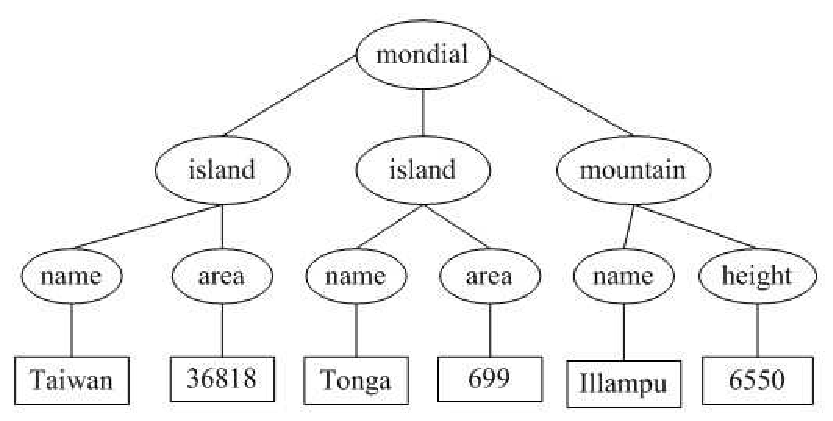
\includegraphics[width=0.4\textwidth]{XML}
\caption{树状结构}\label{fig:xml}
\vspace{\baselineskip}
\end{figure}


其插入图片的代码及其说明如下。
\vspace{1em}\noindent\hrule
\begin{verbatim}
\begin{figure}[htbp]
\centering
\includegraphics[width=0.4\textwidth]{文件名(.eps)}
\caption{标题}\label{标签名(通常为 fig:labelname)}
\vspace{\baselineskip} %表示图与正文空一行
\end{figure}
\end{verbatim}

\noindent\hrule

\begin{verbatim}
figure环境的可选参数[htbp]表示浮动图形所放置的位置,h (here)表示当前位置,t (top)表示页芯顶部,b (bottom)表示页芯底部,p (page)表示单独一页。在Word等软件中,图片通常插入到当前位置,如果当前页的剩余空间不够,图片将被移动到下一页,当前页就会出现很大的空白,其人工调整工作非常不便。由LaTeX提供的浮动图片功能,总是会按h->t->b->p的次序处理选项中的字母,自动调整图片的位置,大大减轻了工作量。
\centering命令将后续内容转换成每行皆居中的格式。
"\includegraphics"的可选参数用来设置图片插入文中的水平宽度,一般表示为正文宽度(\textwidth)的倍数。
\caption命令可选参数“标签名”为英文形式,一般不以图片或表格的数字顺序作为标签,而应包含一定的图片或表格信息,以便于文中引用(若图片、表格、公式、章节和参考文献等在文中出现的先后顺序发生了变化,其标注序号及其文中引用序号也会跟着发生变化,这一点是Word等软件所不能做到的)。另外,图题或表题并不会因为分页而与图片或表格体分置于两页,章节等各级标题也不会置于某页的最底部,LaTeX系统会自动调整它们在正文中的位置,这也是Word等软件所无法匹敌的。
\vspace将产生一定高度的竖直空白,必选参数为负值表示将后续文字位置向上提升,参数值可自行调整。em为长度单位,相当于大写字母M的宽度。\vspace{\baselineskip} 表示图与正文空一行。
引用方法:“见图~\ref{fig:figname}”、“如图~\ref{fig:figname}~所示”等。
\end{verbatim}

\noindent\hrule\vspace{1em}

若需要将~2~张及以上的图片并排插入到一行中,则需要采用\verb|minipage|环境,如图~\ref{fig:dd}~和图~\ref{fig:ds}~所示。
\begin{figure}[htbp]
\centering
\begin{minipage}{0.4\textwidth}
\centering
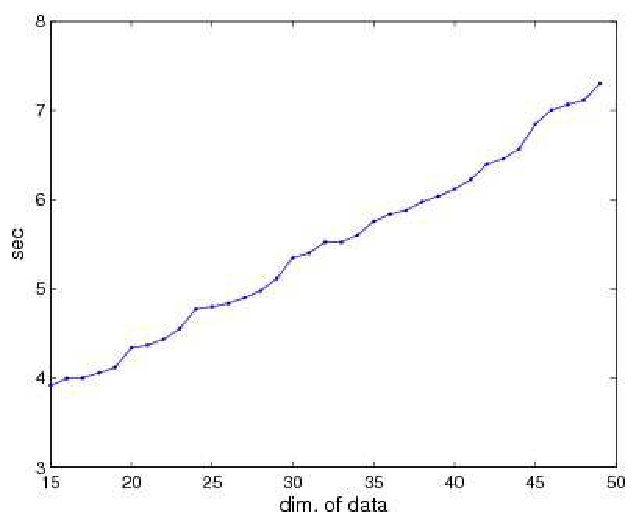
\includegraphics[width=\textwidth]{dataDimensions}
\caption{数据维数的变化}\label{fig:dd}
\end{minipage}
\begin{minipage}{0.4\textwidth}
\centering
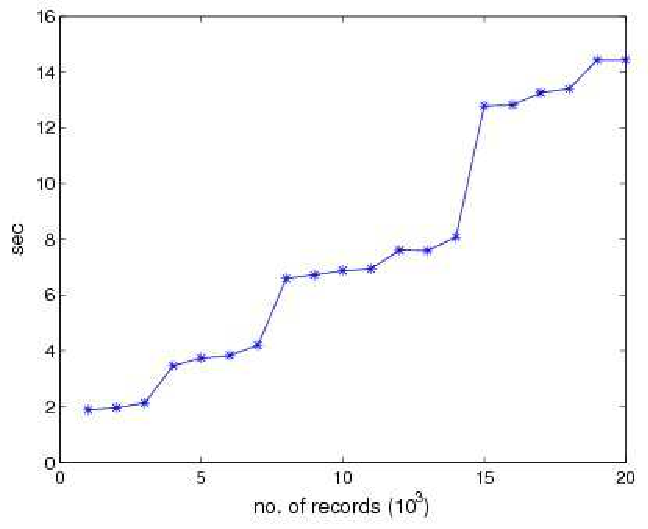
\includegraphics[width=\textwidth]{dataSize}
\caption{数据规模的变化}\label{fig:ds}
\end{minipage}
\vspace{\baselineskip}
\end{figure}

其代码如下所示。
\vspace{1em}\noindent\hrule
\begin{verbatim}
\begin{figure}[htbp]
\centering
\begin{minipage}{0.4\textwidth}
\centering
\includegraphics[width=\textwidth]{文件名}
\caption{标题}\label{fig:f1}
\end{minipage}
\begin{minipage}{0.4\textwidth}
\centering
\includegraphics[width=\textwidth]{文件名}
\caption{标题}\label{fig:f2}
\end{minipage}\vspace{\baselineskip}
\end{figure}
\end{verbatim}

\noindent\hrule

\begin{verbatim}
minipage环境的必选参数用来设置小页的宽度,若需要在一行中插入n个等宽图片,则每个小页的宽度应略小于(1/n)\textwidth。
\end{verbatim}

\noindent\hrule

\section{具有子图的图片插入方法}

图中若含有子图时,需要调用~subfigure~宏包, 如图~\ref{fig:subfig}~所示。
\begin{figure}[htbp]
  \centering
  \subfigure[Data Dimensions]{\label{fig:subfig:datadim}
                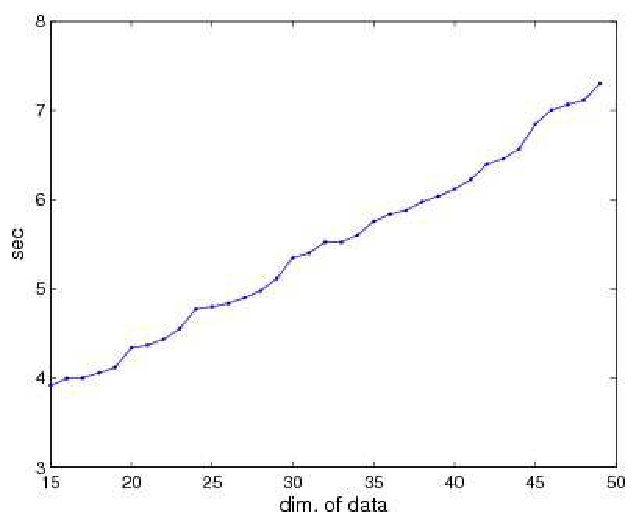
\includegraphics[width=0.4\textwidth]{dataDimensions}}
  \subfigure[Data Size]{\label{fig:subfig:datasize}
                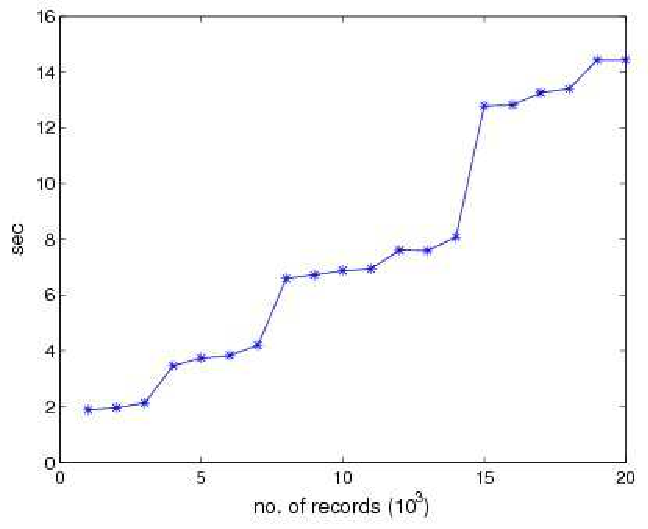
\includegraphics[width=0.4\textwidth]{dataSize}}
  \caption{Scalability of data}\label{fig:subfig}
\vspace{\baselineskip}
\end{figure}

其代码及其说明如下。
\vspace{1em}\noindent\hrule

\begin{verbatim}
\begin{figure}[htbp]
  \centering
  \subfigure[第1个子图标题]{
            \label{第1个子图标签(通常为 fig:subfig1:subsubfig1)}
            \includegraphics[width=0.4\textwidth]{文件名}}
  \subfigure[第2个子图标题]{
            \label{第2个子图标签(通常为 fig:subfig1:subsubfig2)}
            \includegraphics[width=0.4\textwidth]{文件名}}
  \caption{总标题}\label{总标签(通常为 fig:subfig1)}
\vspace{\baselineskip}
\end{figure}
\end{verbatim}

\noindent\hrule

\begin{verbatim}
子图的标签实际上可以随意设定,只要不重复就行。但为了更好的可读性,我们建议fig:subfig:subsubfig格式命名,这样我们从标签名就可以知道这是一个子图引用。
引用方法:总图的引用方法同本章第1节,子图的引用方法用\ref{fig:subfig:subsubfig}来代替。
\end{verbatim}

\noindent\hrule\vspace{1em}

子图的引用示例:如图~\ref{fig:subfig:datadim}~和图~\ref{fig:subfig:datasize}~所示。

若想获得插图方法的更多信息,参见网络上的~\href{ftp://ftp.tex.ac.uk/tex-archive/info/epslatex.pdf}{Using Imported Graphics in \LaTeX and pdf\LaTeX}~文档。 
%%% !Mode:: "TeX:UTF-8"

\chapter{表格的绘制方法}
\section{研究生毕业设计论文的绘表规范}

表应有自明性。表格不加左、右边线。表的编排建议采用国际通行的三线表。表内中文书写使用宋体五号字。

每个表格之上均应有表题(由表序和表名组成)。表序一般按章编排,如第~1~章第一个插表的序号为“表~1-1”等。表序与表名之间空两格,
表名使用中文五号字,居中。表名中不允许使用标点符号,表名后不加标点。
表头设计应简单明了,尽量不用斜线。表头中可采用化学,物理量等专业符号。

全表如用同一单位,则将单位符号移至表头右上角,加圆括号。
表中数据应准确无误,书写清楚。数字空缺的格内加横线“-”(占~2~个数字宽度)。表内文字或数字上、下或左、右相同时,
采用通栏处理方式,不允许用“〃”、“同上”之类的写法。

表内文字使用宋体五号字,垂直居中书写,起行空一格、转行顶格、句末不加标点。
如某个表需要转页接排,在随后的各页上应重复表的编号。编号后加“(续表)”,表题可省略。续表应重复表头。
表格绘制完成之后,与正文空一行。

\section{普通表格的绘制方法}

表格应具有三线表格式,因此需要调用~booktabs~宏包,其标准格式如表~\ref{tab:table1}~所示。
\begin{table}[htbp]
\caption{符合本科生毕业论文绘图规范的表格}\label{tab:table1}
\vspace{0.5em}\centering\wuhao
\begin{tabular}{ccccc}
\toprule[1.5pt]
$D$(in) & $P_u$(lbs) & $u_u$(in) & $\beta$ & $G_f$(psi.in)\\
\midrule[1pt]
 5 & 269.8 & 0.000674 & 1.79 & 0.04089\\
10 & 421.0 & 0.001035 & 3.59 & 0.04089\\
20 & 640.2 & 0.001565 & 7.18 & 0.04089\\
 5 & 269.8 & 0.000674 & 1.79 & 0.04089\\
10 & 421.0 & 0.001035 & 3.59 & 0.04089\\
20 & 640.2 & 0.001565 & 7.18 & 0.04089\\
 5 & 269.8 & 0.000674 & 1.79 & 0.04089\\
10 & 421.0 & 0.001035 & 3.59 & 0.04089\\
20 & 640.2 & 0.001565 & 7.18 & 0.04089\\
 5 & 269.8 & 0.000674 & 1.79 & 0.04089\\
10 & 421.0 & 0.001035 & 3.59 & 0.04089\\
20 & 640.2 & 0.001565 & 7.18 & 0.04089\\
\bottomrule[1.5pt]
\end{tabular}
\vspace{\baselineskip}
\end{table}

其绘制表格的代码及其说明如下。
\vspace{1em}\noindent\hrule

\begin{verbatim}
\begin{table}[htbp]
\caption{表标题}\label{标签名(通常为 tab:tablename)}
\vspace{0.5em}\centering\wuhao
\begin{tabular}{cc...c}
\toprule[1.5pt]
表头第1个格   & 表头第2个格   & ... & 表头第n个格  \\
\midrule[1pt]
表中数据(1,1) & 表中数据(1,2) & ... & 表中数据(1,n)\\
表中数据(2,1) & 表中数据(2,2) & ... & 表中数据(2,n)\\
表中数据(3,1) & 表中数据(3,2) & ... & 表中数据(3,n)\\
表中数据(4,1) & 表中数据(4,2) & ... & 表中数据(4,n)\\
...................................................\\
表中数据(m,1) & 表中数据(m,2) & ... & 表中数据(m,n)\\
\bottomrule[1.5pt]
\end{tabular}
\vspace{\baselineskip}
\end{table}
\end{verbatim}

\noindent\hrule

\begin{verbatim}
table环境是一个将表格嵌入文本的浮动环境。
\wuhao命令将表格的字号设置为五号字(10.5pt),在绘制表格结束退出时,不需要将字号再改回为\xiaosi,正文字号默认为小四号字(12pt)。
tabular环境的必选参数由每列对应一个格式字符所组成:c表示居中,l表示左对齐,r表示右对齐,其总个数应与表的列数相同。此外,@{文本}可以出现在任意两个上述的列格式之间,其中的文本将被插入每一行的同一位置。表格的各行以\\分隔,同一行的各列则以&分隔。
\toprule、\midrule和\bottomrule三个命令是由booktabs宏包提供的,其中\toprule和\bottomrule分别用来绘制表格的第一条(表格最顶部)和第三条(表格最底部)水平线,\midrule用来绘制第二条(表头之下)水平线,且第一条和第三条水平线的线宽为1.5pt,第二条水平线的线宽为1pt。
引用方法:“如表~\ref{tab:tablename}~所示”。
\end{verbatim}

\noindent\hrule

\section{长表格的绘制方法}

长表格是当表格在当前页排不下而需要转页接排的情况下所采用的一种表格环境。若长表格仍按照普通表格的绘制方法来获得,
其所使用的\verb|table|浮动环境无法实现表格的换页接排功能,表格下方过长部分会排在表格第1页的页脚以下。为了能够实现长表格的转页接排功能,
需要调用~longtable~宏包,由于长表格是跨页的文本内容,因此只需要单独的\verb|longtable|环境,所绘制的长表格的格式如表~\ref{tab:table2}~所示。

此长表格~\ref{tab:table2}~第~2~页的标题“编号(续表)”和表头是通过代码自动添加上去的,无需人工添加,若表格在页面中的竖直位置发生了变化,长表格在第~2~页
及之后各页的标题和表头位置能够始终处于各页的最顶部,也无需人工调整,\LaTeX~系统的这一优点是~Word~等软件所无法企及的。

下段内容是为了让下面的长表格分居两页,看到表标题“编号(续表)”的效果。摘录于《你若安好,便是晴天 -- 林徽因传》片段:

她叫林徽因,出生于杭州,是许多人梦中期待的白莲。她在雨雾之都伦敦,发生过一场空前绝后的康桥之恋。她爱过三个男子,爱得清醒,也爱得平静。徐志摩为她徜徉在康桥,深情地等待一场旧梦可以归来。梁思成与她携手走过千山万水,为完成使命而相约白头。金岳霖为她终身不娶,痴心不改地守候一世。可她懂得人生飘忽不定,要学会随遇而安。
真正的平静,不是避开车马喧嚣,而是在心中修篱种菊。尽管如流往事,每一天都涛声依旧,只要我们消除执念,便可寂静安然。愿每个人在纷呈世相中不会迷失荒径,可以端坐磐石上,醉倒落花前。
如果可以,请让我预支一段如莲的时光,哪怕将来某一天加倍偿还。这个雨季会在何时停歇,无从知晓。但我知道,你若安好,便是晴天。					
\wuhao\begin{longtable}{ccc}
\caption{天津大学各学院名称一览}\label{tab:table2}
 \vspace{0.5em}\\
\toprule[1.5pt] 学院名称 & 网址 & 联系电话  \\ \midrule[1pt]
\endfirsthead
\multicolumn{3}{c}{表~\thetable(续表)}\vspace{0.5em}\\
\toprule[1.5pt] 学院名称 & 网址 & 联系电话  \\ \midrule[1pt]
\endhead
\bottomrule[1.5pt]
\endfoot
机械工程学院& \url{http://tdjxxy.tju.edu.cn/}& 87401979\\
精密仪器与光电子工程学院&  \url{http://www2.tju.edu.cn/colleges/precision/cn/}& 27404775\\
电子信息工程学院& \url{http://www.tju.edu.cn/seie}& 27406956\\
电气与自动化工程学院& \url{http://www2.tju.edu.cn/colleges/automate/}& 27405477\\
建筑工程学院& \url{http://www2.tju.edu.cn/colleges/civil/}& 27404072\\
化工学院& \url{http://chemeng.tju.edu.cn/}& 27403389\\
材料科学与工程学院& \url{http://mse.tju.edu.cn}& 27406693 \\
建筑学院& \url{http://hgw022072.chinaw3.com/}& 27402724-2111\\
求是学部\\
管理与经济学部&	\url{ http://sm.tju.edu.cn}& 27403423\\
理学院& \url{ http://www.tju.edu.cn/science/}& 27404118\\
文法学院& \url{ http://www2.tju.edu.cn/colleges/sociology/new/}& 27403691\\
软件学院& \url{http://scs.tju.edu.cn}& 87401540\\
计算机科学与技术学院& \url{http://cs.tju.edu.cn/}& 27406538\\
马克思主义学院& \url{http://www2.tju.edu.cn/colleges/marxism/}& 27405348\\
环境科学与工程学院& \url{http://www.tju.edu.cn/see}& 87402072\\
药物科学与技术学院& \url{http://www2.tju.edu.cn/colleges/pharmtier/}& 87401830\\
教育学院& \url{http://soe.tju.edu.cn/}& 27401028\\
职业技术教育学院& \url{http://202.113.0.248:8888}\\
继续教育学院& \url{http://aectu.tju.edu.cn/}& 27406298\\
仁爱学院& \url{http://www.tjrac.edu.cn/}& 68579990\\
农业与生物工程学院& \url{http://202.113.13.169/site/nongxueyuan/}& 87402171\\
国际教育学院 & \url{http://www.ietju.com/}& 27406147\\
网络教育学院 & \url{http://www.etju.com/}& 27426952 \\

\end{longtable}\xiaosi
\vspace{\baselineskip}

绘制长表格的代码及其说明如下。
\vspace{1em}\noindent\hrule

\begin{verbatim}
\wuhao\begin{longtable}{cc...c}
\caption{表标题}\label{标签名(通常为 tab:tablename)}\\
\toprule[1.5pt] 表头第1个格 & 表头第2个格 & ... & 表头第n个格\\ \midrule[1pt]
\endfirsthead
\multicolumn{n}{c}{表~\thetable(续表)}\vspace{0.5em}\\
\toprule[1.5pt] 表头第1个格 & 表头第2个格 & ... & 表头第n个格\\ \midrule[1pt]
\endhead
\bottomrule[1.5pt]
\endfoot
表中数据(1,1) & 表中数据(1,2) & ... & 表中数据(1,n)\\
表中数据(2,1) & 表中数据(2,2) & ... & 表中数据(2,n)\\
...................................................\\
表中数据(m,1) & 表中数据(m,2) & ... & 表中数据(m,n)\\
\end{longtable}\xiaosi
\end{verbatim}

\noindent\hrule
\begin{verbatim}
在绘制长表格的前面留出一个空白行,并在第2行的一开始全局定义长表格的字号为五号字,这样能够保证长表格之前段落的行距保持不变。
在绘制长表格结束后,需要\xiaosi命令重新将字号改为小四号字。
\endhead之前的文字描述的是第2页及其之后各页的标题或表头;
\endfirsthead之前的文字描述的是第1页的标题和表头,若无此命令,则第1页的表头和标题由\endhead命令确定;
同理,\endfoot之前的文字描述的是除最后一页之外每页的表格底部内容;
\endlastfoot之前的文字描述的是最后一页的表格底部内容,若无此命令,
则最后一页的表格底部内容由\endfoot命令确定;由于规范中长表格每页底部内容均相同(水平粗线),因此模板中没有用到\endlastfoot命令。
\end{verbatim}

\noindent\hrule
\section{列宽可调表格的绘制方法}
论文中能用到列宽可调表格的情况共有两种:一种是当插入的表格某一单元格内容过长以至于一行放不下的情况,
另一种是当对公式中首次出现的物理量符号进行注释的情况。这两种情况都需要调用~tabularx~宏包。下面将分别对这两种情况下可调表格的绘制方法进行阐述。
\subsection{表格内某单元格内容过长的情况}

首先给出这种情况下的一个例子如表~\ref{tab:table3}~所示。
\begin{table}[htbp]
\caption{最小的三个正整数的英文表示法}\label{tab:table3}
\vspace{0.5em}\wuhao
\begin{tabularx}{\textwidth}{llX}
\toprule[1.5pt]
Value & Name & Alternate names, and names for sets of the given size\\\midrule[1pt]
1 & One & ace, single, singleton, unary, unit, unity\\
2 & Two & binary, brace, couple, couplet, distich, deuce, double, doubleton, duad, duality, duet, duo, dyad, pair, snake eyes, span, twain, twosome, yoke\\
3 & Three & deuce-ace, leash, set, tercet, ternary, ternion, terzetto, threesome, tierce, trey, triad, trine, trinity, trio, triplet, troika, hat-trick\\\bottomrule[1.5pt]
\end{tabularx}
\vspace{\baselineskip}
\end{table}
绘制这种表格的代码及其说明如下。
\vspace{1em}\noindent\hrule
\begin{verbatim}
\begin{table}[htbp]
\caption{表标题}\label{标签名(通常为 tab:tablename)}
\vspace{0.5em}\wuhao
\begin{tabularx}{\textwidth}{l...X...l}
\toprule[1.5pt]
表头第1个格   & ... & 表头第X个格   & ... & 表头第n个格  \\
\midrule[1pt]
表中数据(1,1) & ... & 表中数据(1,X) & ... & 表中数据(1,n)\\
表中数据(2,1) & ... & 表中数据(2,X) & ... & 表中数据(2,n)\\
.........................................................\\
表中数据(m,1) & ... & 表中数据(m,X) & ... & 表中数据(m,n)\\
\bottomrule[1.5pt]
\end{tabularx}
\vspace{\baselineskip}
\end{table}
\end{verbatim}

\noindent\hrule
\begin{verbatim}
tabularx环境共有两个必选参数:第1个参数用来确定表格的总宽度,这里取为排版表格能达到的最大宽度——正文宽度\textwidth;第2个参数用来确定每列格式,其中标为X的项表示该列的宽度可调,其宽度值由表格总宽度确定。
标为X的列一般选为单元格内容过长而无法置于一行的列,这样使得该列内容能够根据表格总宽度自动分行。若列格式中存在不止一个X项,则这些标为X的列的列宽相同,因此,一般不将内容较短的列设为X。
标为X的列均为左对齐,因此其余列一般选为l(左对齐),这样可使得表格美观,但也可以选为c或r。
\end{verbatim}

\noindent\hrule
\subsection{对物理量符号进行注释的情况}
为使得对公式中物理量符号注释的转行与破折号“———”后第一个字对齐,此处最好采用表格环境。此表格无任何线条,左对齐,
且在破折号处对齐,一共有“式中”二字、物理量符号和注释三列,表格的总宽度可选为文本宽度,因此应该采用\verb|tabularx|环境。
由\verb|tabularx|环境生成的对公式中物理量符号进行注释的公式如式(\ref{eq:1})所示。
%\vspace*{10pt}

\begin{equation}\label{eq:1}
\ddot{\boldsymbol{\rho}}-\frac{\mu}{R_{t}^{3}}\left(3\mathbf{R_{t}}\frac{\mathbf{R_{t}\rho}}{R_{t}^{2}}-\boldsymbol{\rho}\right)=\mathbf{a}
\end{equation}

\begin{tabularx}{\textwidth}{@{}l@{\quad}r@{———}X@{}}
式中& $\bm{\rho}$ &追踪飞行器与目标飞行器之间的相对位置矢量;\\
&  $\bm{\ddot{\rho}}$&追踪飞行器与目标飞行器之间的相对加速度;\\
&  $\mathbf{a}$   &推力所产生的加速度;\\
&  $\mathbf{R_t}$ & 目标飞行器在惯性坐标系中的位置矢量;\\
&  $\omega_{t}$ & 目标飞行器的轨道角速度;\\
&  $\mathbf{g}$ & 重力加速度,$=\frac{\mu}{R_{t}^{3}}\left(
3\mathbf{R_{t}}\frac{\mathbf{R_{t}\rho}}{R_{t}^{2}}-\bm{\rho}\right)=\omega_{t}^{2}\frac{R_{t}}{p}\left(
3\mathbf{R_{t}}\frac{\mathbf{R_{t}\rho}}{R_{t}^{2}}-\bm{\rho}\right)$,这里~$p$~是目标飞行器的轨道半通径。
\end{tabularx}
\vspace{\wordsep}

其中生成注释部分的代码及其说明如下。

\vspace{1em}\noindent\hrule

\begin{verbatim}
\begin{tabularx}{\textwidth}{@{}l@{\quad}r@{— — —}X@{}}
式中 & symbol-1 & symbol-1的注释内容;\\
     & symbol-2 & symbol-2的注释内容;\\
     .............................;\\
     & symbol-m & symbol-m的注释内容。
\end{tabularx}\vspace{\wordsep}
\end{verbatim}

\noindent\hrule

\begin{verbatim}
tabularx环境的第1个参数选为正文宽度,第2个参数里面各个符号的意义为:
    第1个@{}表示在“式中”二字左侧不插入任何文本,“式中”二字能够在正文中左对齐,若无此项,则“式中”二字左侧会留出一定的空白;
    @{\quad}表示在“式中”和物理量符号间插入一个空铅宽度的空白;
    @{— — —}实现插入破折号的功能,它由三个1/2的中文破折号构成;
    第2个@{}表示在注释内容靠近正文右边界的地方能够实现右对齐。
\end{verbatim}

\noindent\hrule\vspace{1em}

由此方法生成的注释内容应紧邻待注释公式并置于其下方,因此不能将代码放入\verb|table|浮动环境中。但此方法不能实现自动转页接排,
可能会在当前页剩余空间不够时,全部移动到下一页而导致当前页出现很大空白。因此在需要转页处理时,还请您手动将需要转页的代码放入一个
新的\verb|tabularx|环境中,将原来的一个\verb|tabularx|环境拆分为两个\verb|tabularx|环境。

若想获得绘制表格的更多信息,参见网络上的~\href{http://www.tug.org/pracjourn/2007-1/mori/}{Tables in \LaTeXe: Packages and Methods}~文档。


%%% !Mode:: "TeX:UTF-8"

\chapter{数学公式的输入方法}
\section{研究生毕业设计论文的公式规范}

论文中的公式应另起行,原则上应居中书写,与周围文字留有足够的空间区分开。
若公式前有文字(如“解”、“假定”等),文字空两格写,公式仍居中写。公式末不加标点。

公式应标注序号,并将序号置于括号内。 公式序号按章编排,如第~1~章第一个公式序号为“(1-1)”。公式的序号右端对齐。

公式较长时最好在等号“=”处转行,如难实现,则可在~$+$、$-$、$\times$、$\div$~运算符号处转行,转行时运算符号仅书写于转行式前,不重复书写。

文中引用公式时,一般用“见式~(1-1)”或“由公式~(1-1)”。

公式中用斜线表示“除”的关系时应采用括号,以免含糊不清,如~$a/(b\cos x)$。通常“乘”的关系在前,如~$a\cos x/b$而不写成~$(a/b)\cos x$。

不能用文字形式表示等式,如:$\textnormal{刚度}=\frac{{\textnormal{受力}}}{{\textnormal{受力方向的位移}}}$。

对于数学公式的输入方法,网络上有一个比较全面权威的文档\textbf{~\href{http://tug.ctan.org/cgi-bin/ctanPackageInformation.py?id=voss-mathmode}{Math mode}}~请大家事先大概浏览一下。下面将对学位论文中主要用到的数学公式排版形式进行阐述。

\section{生成~\LaTeX~数学公式的两种方法}
对于先前没有接触过~\LaTeX~的人来说,编写~\LaTeX~数学公式是一件很繁琐的事,尤其是对复杂的数学公式来说,更可以说是一件难以完成的任务。
实际上,生成~\LaTeX~数学公式有两种较为简便的方法,一种是基于~MathType~数学公式编辑器的方法,另一种是基于~MATLAB~商业数学软件的方法,
下面将分别对这两种数学公式的生成方法作一下简单介绍。

\subsection{基于~MathType~软件的数学公式生成方法}
MathType~是一款功能强大的数学公式编辑器软件,能够用来在文本环境中插入~Windows OLE~图形格式的复杂数学公式,所以应用比较普遍。但此软件只有~30~天的试用期,之后若再继续使用则需要付费购买才行。网络上有很多破解版的~MathType~软件可供下载免费使用,
笔者推荐下载安装版本号在~6.5~之上的中文破解版。

在安装好~MathType~之后,若在输入窗口中编写数学公式,复制到剪贴板上的仍然是图形格式的对象。
若希望得到可插入到~\LaTeX~编辑器中的文本格式对象,则需要对~MathType~软件做一下简单的设置:在~MathType~最上排的按钮中依次选择“参数选项
$\to$转换”,在弹出的对话窗中选中“转换到其它语言(文字):”,在转换下拉框中选择“Tex~--~--~LaTeX 2.09 and later”,并将对话框最下方的两个复选框全部勾掉,点击确定,这样,再从输入窗口中复制出来的对象就是文本格式的了,就可以直接将其粘贴到~\LaTeX~
编辑器中了。按照这种方法生成的数学公式两端分别有标记\verb|\[|和标记\verb|\]|,在这两个标记之间才是真正的数学公式代码。

若希望从~MathType~输入窗口中复制出来的对象为图形格式,则只需再选中“公示对象(Windows OLE~图形)”即可。

\subsection{基于~MATLAB~软件的数学公式生成方法}

MATLAB~是矩阵实验室(Matrix Laboratory)的简称,是美国~MathWorks~公司出品的商业数学软件。它是当今科研领域最常用的应用软件之一,
具有强大的矩阵计算、符号运算和数据可视化功能,是一种简单易用、可扩展的系统开发环境和平台。

MATLAB~中提供了一个~latex~函数,它可将符号表达式转化为~\LaTeX~数学公式的形式。其语法形式为~latex(s),其中,~s~为符号表达式,
之后再将~latex~函数的运算结果直接粘贴到~\LaTeX~编辑器中。从~\LaTeX~数学公式中可以发现,其中可能包含如下符号组合:

\begin{verbatim*}
\qquad=两个空铅(quad)宽度
\quad=一个空铅宽度
\;=5/18空铅宽度
\:=4/18空铅宽度
\,=3/18空铅宽度
\!=-3/18空铅宽度
\ =一个空格
\end{verbatim*}

所以最好将上述符号组合从数学公式中删除,从而使数学公式显得匀称美观。

对于~Word~等软件的使用者来说,在我们通过~MATLAB~运算得到符号表达式形式的运算结果时,在~Word~中插入运算结果需要借助于~MathType~软件,
通过在~MathType~中输入和~MATLAB~运算结果相对应的数学表达形式,之后再将~MathType~数学表达式转换为图形格式粘贴到~Word~中。实际上,
也可以将~MATLAB~中采用~latex~函数运行的结果直接粘贴到~MathType~中,再继续上述步骤,这样可以大大节省输入公式所需要的时间。
此方法在~MathType~6.5c~上验证通过,若您粘入到~MathType~中的仍然为从~MATLAB~中导入的代码,请您更新~MathType~软件。

\section{数学字体}
在数学模式下,常用的数学字体命令有如下几种:

\begin{verbatim}
\mathnormal或无命令 用数学字体打印文本;
\mathit             用斜体(\itshape)打印文本;
\mathbf             用粗体(\bfseries)打印文本;
\mathrm             用罗马体(\rmfamily)打印文本;
\mathsf             用无衬线字体(\sffamily)打印文本;
\mathtt             用打印机字体(\ttfamily)打印文本;
\mathcal            用书写体打印文本;
\end{verbatim}

在学位论文撰写中,只需要用到上面提到的~\verb|\mathit|、\verb|\mathbf|~和~\verb|\mathrm|~命令。若要得到~Times New Roman~的数学字体,则需要调用~txfonts~宏包(此宏包实际上采用的是~Nimbus Roman No9 L~字体,
它是开源系统中使用的免费字体,其字符字体与~Times New Roman~字体几乎完全相同);若要得到粗体数学字体,则需要调用~bm~宏包。表~\ref{tab:fonts}~中分别列出了得到阿拉伯数字、拉丁字母和希腊字母
各种数学字体的命令。

\begin{table}[htbp]
\caption{常用数学字体命令一览}\label{tab:fonts}
\vspace{0.5em}\centering\wuhao
\begin{tabular}{llll}
\toprule
 & 阿拉伯数字\&大写希腊字母 & 大小写拉丁字母 & 小写希腊字母  \\
\midrule
斜体 & \verb|\mathit{}| & \verb|无命令| & \verb|无命令|\\
粗斜体 & \verb|\bm{\mathit{}}| & \verb|\bm{}| & \verb|\bm{}|\\
直立体 & \verb|无命令| & \verb|\mathrm{}| & \verb|字母后加up|\\
粗体 & \verb|\mathbf{}或\bm{}| & \verb|\mathbf{}| & \verb|\bm{字母后加up}|\\
\bottomrule
\end{tabular}
\vspace{\baselineskip}
\end{table}

\noindent 下面列出了一些应采用直立数学字体的数学常数和数学符号。

\vspace{-0.5em}\begin{center}\begin{tabularx}{0.7\textwidth}{XX}
$\mathrm{d}$、 $\mathrm{D}$、 $\mathrm{p}$~———微分算子 & $\mathrm{e}$~———自然对数之底数\\
$\mathrm{i}$、 $\mathrm{j}$~———虚数单位 & $\piup$———圆周率\\
\end{tabularx}\end{center}

\section{行内公式}
出现在正文一行之内的公式称为行内公式,例如~$f(x)=\int_{a}^{b}\frac{\sin{x}}{x}\mathrm{d}x$。对于非矩阵和非多行形式的行内公式,一般不会使得行距发生变化,而~Word~等软件却会根据行内公式的竖直距离而自动调节行距,如图~\ref{fig:hangju}~所示。

\begin{figure}[htbp]
\centering
\subfigure[由~\LaTeX~系统生成的行内公式]{\label{fig:subfig:latex}
                \fbox{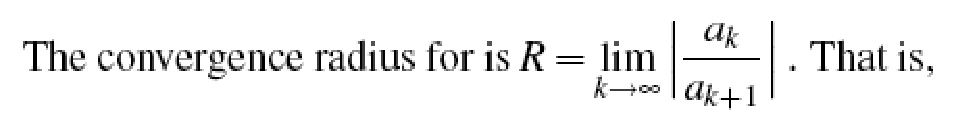
\includegraphics[width=0.55\textwidth]{latex}}}
\subfigure[由~Word软件生成的~.doc~格式行内公式]{\label{fig:subfig:word}
                \fbox{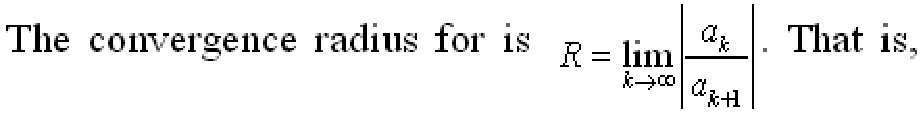
\includegraphics[width=0.55\textwidth]{word}}}
\subfigure[由~Word软件生成的~.pdf~格式行内公式]{\label{fig:subfig:pdf}
                \fbox{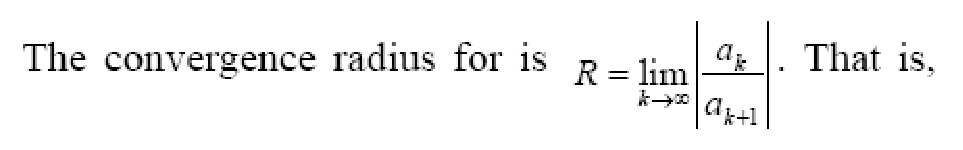
\includegraphics[width=0.55\textwidth]{pdf}}}

\caption{由~\LaTeX~和~Word~生成的~3~种行内公式屏显效果}\label{fig:hangju}
\vspace{-1em}
\end{figure}

这三幅图分别为~\LaTeX~和~Word~生成的行内公式屏显效果,从图中可看出,在~\LaTeX~文本含有公式的行内,在正文与公式之间对接工整,行距不变;而在~Word~文本含有公式的行内,在正文与公式之间对接不齐,行距变大。因此从这一点来说,
\LaTeX~系统在数学公式的排版上具有很大优势。

\LaTeX~提供的行内公式最简单、最有效的方法是采用~\TeX~本来的标记———开始和结束标记都写作~\$,例如本段开始的例子可由下面的输入得到。
\verb|$f(x)=\int_{a}^{b}\frac{\sin{x}}{x}\mathrm{d}x$|

\section{行间公式}
位于两行之间的公式称为行间公式,每个公式都是一个单独的段落,例如
\[\int_a^b{f\left(x\right)\mathrm{d}x}=\lim_{\left\|\Delta{x_i}\right\|\to 0}\sum_i{f\left(\xi_i\right)\Delta{x_i}}\]
除人工编号外,\LaTeX~各种类型行间公式的标记见表~\ref{tab:eqtag}。
\begin{table}[htbp]
\caption{各种类型行间公式的标记}\label{tab:eqtag}
\vspace{0.5em}\centering\wuhao
\begin{tabularx}{\textwidth}{cll}
\toprule
& 无编号 & 自动编号\\
\midrule
单行公式& \verb|\begin{displaymath}... \end{displaymath}|& \verb|\begin{equation}... \end{equation}|\\
        & 或~\verb|\[...\]| & \\
多行公式& \verb|\begin{eqnarray*}... \end{eqnarray*}|& \verb|\begin{eqnarray}... \end{eqnarray}|\\
\bottomrule
\end{tabularx}
\end{table}

另外,在自动编号的某行公式行尾添加标签~\verb|\nonumber|,可将该行转换为无编号形式。

行间多行公式需采用~\verb|eqnarray|~或~\verb|eqnarray*|~环境,它默认是一个列格式为~\verb|rcl|~的~3~列矩阵,并且中间列的字号要小一些,因此通常只将需要对齐的运算符号(通常为等号“=”)置于中间列。

\section{可自动调整大小的定界符}
若在左右两个定界符之前分别添加命令~\verb|\left|~和~\verb|\right|,则定界符可根据所包围公式大小自动调整其尺寸,这可从式(\ref{nodelimiter})和式(\ref{delimiter})中看出。
\begin{equation}\label{nodelimiter}
(\sum_{k=\frac12}^{N^2})
\end{equation}
\begin{equation}\label{delimiter}
\left(\sum_{k=\frac12}^{N^2}\right)
\end{equation}
式(\ref{nodelimiter})和式(\ref{delimiter})是在~\LaTeX~中分别输入如下代码得到的。
\begin{verbatim}
(\sum_{k=\frac12}^{N^2})
\left(\sum_{k=\frac12}^{N^2}\right)
\end{verbatim}
\verb|\left|~和~\verb|\right|~总是成对出现的,若只需在公式一侧有可自动调整大小的定界符,则只要用“.”代替另一侧那个无需打印出来的定界符即可。

若想获得关于此部分内容的更多信息,可参见~\href{http://tug.ctan.org/cgi-bin/ctanPackageInformation.py?id=voss-mathmode}{Math mode}~文档的第~8~章“Brackets, braces and parentheses”。

\section{数学重音符号}
数学重音符号通常用来区分同一字母表示的不同变量,输入方法如下(需要调用~\verb|amsmath|~宏包):

\vspace{0.5em}\noindent\wuhao\begin{tabularx}{\textwidth}{Xc|Xc|Xc}
 \verb|\acute| & $\acute{a}$ & \verb|\mathring| & $\mathring{a}$ & \verb|\underbrace| & $\underbrace{a}$ \\
 \verb|\bar| & $\bar{a}$ & \verb|\overbrace| & $\overbrace{a}$ & \verb|\underleftarrow| & $\underleftarrow{a}$ \\
 \verb|\breve| & $\breve{a}$ & \verb|\overleftarrow| & $\overleftarrow{a}$ & \verb|\underleftrightarrow| & $\underleftrightarrow{a}$ \\
 \verb|\check| & $\check{a}$ & \verb|\overleftrightarrow| & $\overleftrightarrow{a}$ & \verb|\underline| & $\underline{a}$ \\
 \verb|\dddot| & $\dddot{a}$ & \verb|\overline| & $\overline{a}$ & \verb|\underrightarrow| & $\underrightarrow{a}$ \\
 \verb|\ddot| & $\ddot{a}$ & \verb|\overrightarrow| & $\overrightarrow{a}$ & \verb|\vec| & $\vec{a}$ \\
 \verb|\dot| & $\dot{a}$ & \verb|\tilde| & $\tilde{a}$ & \verb|\widehat| & $\widehat{a}$ \\
 \verb|\grave| & $\grave{a}$ & \verb|\underbar| & $\underbar{a}$ & \verb|\widetilde| & $\widetilde{a}$ \\
 \verb|\hat| & $\hat{a}$
\end{tabularx}\vspace{0.5em}
\xiaosi 当需要在字母~$i$~和~$j$~的上方添加重音符号时,为了去掉这两个字母顶上的小点,这两个字母应该分别改用~\verb|\imath|~和~\verb|\jmath|。

如果遇到某些符号不知道该采用什么命令能输出它时,则可通过~\href{http://detexify.kirelabs.org/classify.html}{Detexify$^2$~网站}来获取符号命令。若用鼠标左键在此网页的方框区域内画出你所要找的符号形状,则会在网页右方列出和你所画符号形状相近的~5~个符号及其相对应的~\LaTeX~输入命令。若所列出的符号中不包括你所要找的符号,还可通过点击“Select from the complete list!”的链接以得分从低到高的顺序列出所有符号及其相对应的~\LaTeX~输入命令。

最后,建议大家还以~\href{http://tug.ctan.org/cgi-bin/ctanPackageInformation.py?id=voss-mathmode}{Math mode}~这篇~pdf~文档作为主要参考。若要获得最为标准、美观的数学公式排版形式,可以查查文档中是否有和你所要的排版形式相同或相近的代码段,通过修改代码段以获得你所要的数学公式排版形式。


%%% !Mode:: "TeX:UTF-8"

\chapter{罗列和定理环境使用方法}

\section{单层罗列环境}
天津大学学位论文一般可采用两种罗列环境:一种是并列条目有同样标签的~\verb|itemize|~罗列环境,另一种是具有自动排序编号符号的~\verb|enumerate|~罗列环境。这两种罗列环境的样式参数可参考图~\ref{fig:list}。
\begin{figure}[htbp]
\centering
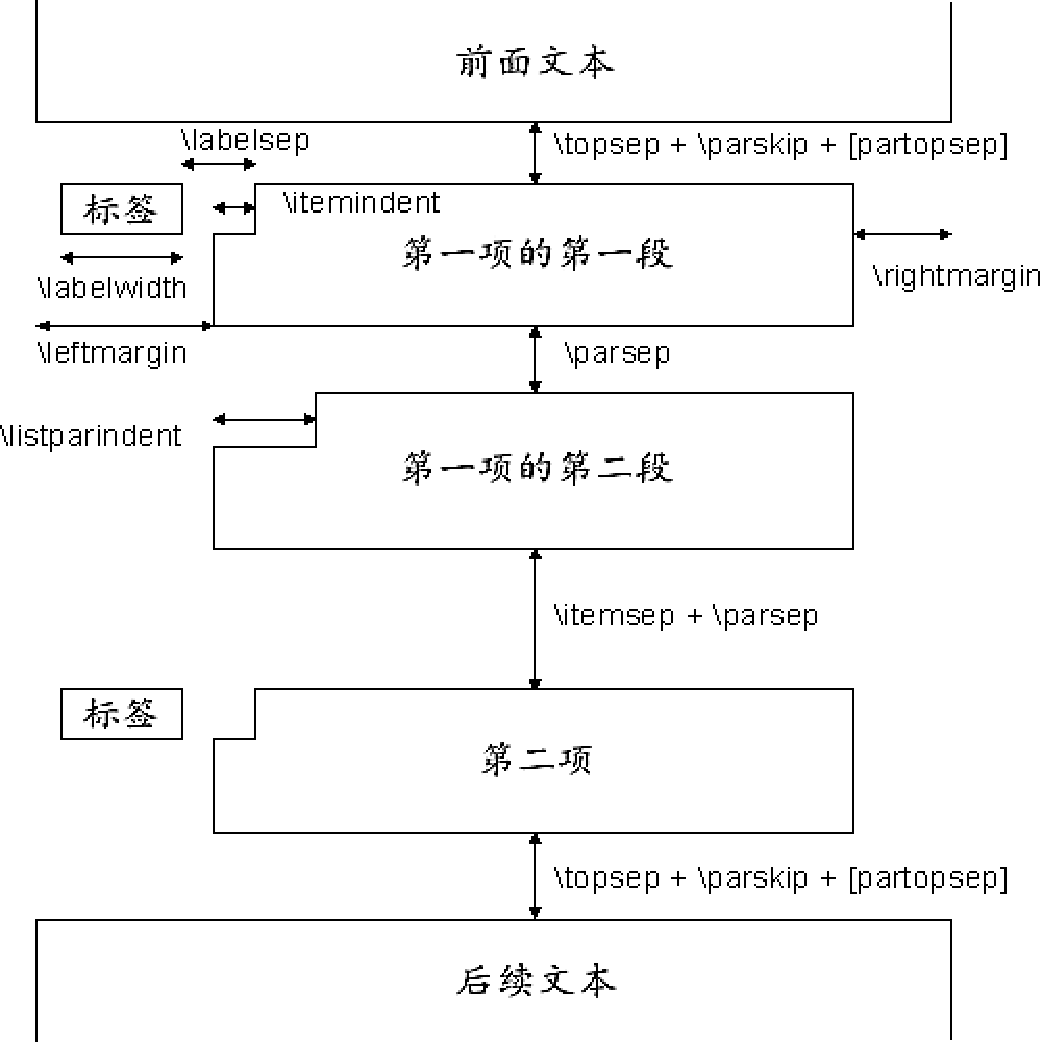
\includegraphics[width = 0.6\textwidth]{list}
\caption{罗列环境参数示意图}\label{fig:list}\vspace{-1em}
\end{figure}

通过调用~enumitem~宏包可以很方便地控制罗列环境的布局,其~format.tex~文件中的~\verb|\setitemize|~和~\verb|\setenumerate|~命令分别用来设置~\verb|itemize|~和~\verb|enumerate|~环境的样式参数。采用~\verb|itemize|~单层罗列环境的排版形式如下:

\begin{itemize}
\item 第一个条目文本内容
\item 第二个条目文本内容
\item 第三个条目文本内容
\end{itemize}

其代码如下

\begin{verbatim}
\begin{itemize}
  \item 第一个条目文本内容
  \item 第二个条目文本内容
  ...
  \item 第三个条目文本内容
\end{itemize}
\end{verbatim}

采用~\verb|enumerate|~单层罗列环境的排版形式如下:

\begin{enumerate}
\item 第一个条目文本内容
\item 第二个条目文本内容
\item 第三个条目文本内容
\end{enumerate}

其代码如下

\begin{verbatim}
\begin{enumerate}
  \item 第一个条目文本内容
  \item 第二个条目文本内容
  ...
  \item 第三个条目文本内容
\end{enumerate}
\end{verbatim}



\section{定理环境}

\begin{definition}[谱半径]\label{def:def1}
  称~$n$~阶方阵~$\mathbf{A}$~的全体特征值~$\lambda_1,\cdots,\lambda_n$~组成的集合为~$\mathbf{A}$~的谱,称
  $$\rho(\mathbf{A})=\max{\{|\lambda_1|,\cdots,|\lambda_n|\}}$$
\end{definition}
\begin{theorem}[相似充要条件]\label{lemma:l1}
  方阵$A$和$B$相似的充要条件是:~$A$~和~$B$~有全同的不变因子。
\end{theorem}
\begin{corollary}[推论1]\label{cor:cor1}
在赋范空间~$(X,\|\cdot\|)$~上定义~$d(x,y)=\|x-y\|$, 对任意~$x,y\in X$,~则~$(X,d)$~是距离空间。
\end{corollary}
\begin{proof}
  只需证明~$d(x,y)$~是距离。
\end{proof}
\newpage

定义代码如下:
\begin{verbatim}
 \begin{definition}[谱半径]\label{def:def1}
  称~$n$~阶方阵~$\mathbf{A}$~的全体特征值
  $\lambda_1,\cdots,\lambda_n$组成的集合为~$\mathbf{A}$~的谱,称
  $$\rho(\mathbf{A})=\max{\{|\lambda_1|,\cdots,|\lambda_n|\}}$$
\end{definition}
\end{verbatim}
\noindent\hrule

\vspace{0.1em}\noindent\hrule
\vspace{1em}
定理代码如下:
\begin{verbatim}
\begin{theorem}[相似充要条件]\label{lemma:l1}
  方阵$A$和$B$相似的充要条件是:$A$和$B$有全同的不变因子。
\end{theorem}
\end{verbatim}
\noindent\hrule\vspace{0.1em}

\noindent\hrule
\vspace{1em}
推论和证明代码如下:
\begin{verbatim}
\begin{corollary}[推论1]\label{cor:cor1}
在赋范空间~$(X,\|\cdot\|)$~上定义$d(x,y)=\|x-y\|$,
对任意$x,y\in X$,则$(X,d)$是距离空间。
\end{corollary}
\begin{proof}
  只需证明$d(x,y)$是距离。
\end{proof}
\end{verbatim}
\noindent\hrule\vspace{1em}

定理定义[]中是可选参数,用来说明定理的名称。其他环境格式书写与上面定理、定义、推论格式相同,可自己调用其他环境。
若需要书写定理定义等内容,而且带有顺序编号,需要采用如下环境。除了~\verb|proof|~环境之外,其余~9~个环境都可以有一个可选参数作为附加标题。

\begin{center}
\vspace{0.5em}\noindent\wuhao\begin{tabularx}{0.7\textwidth}{lX|lX}
定理 & \verb|theorem|~环境 & 定义 & \verb|definition|~环境 \\
例 & \verb|example|~环境 & 算法 & \verb|algorithm|~环境 \\
公理 & \verb|axiom|~环境 & 命题 & \verb|proposition|~环境 \\
引理 & \verb|lemma|~环境 & 推论 & \verb|corollary|~环境 \\
注解 & \verb|remark|~环境 & 证明 & \verb|proof|~环境 \\
\end{tabularx}
\end{center} 
%%% !Mode:: "TeX:UTF-8"

\markboth{总结与展望}{总结与展望}
%\addcontentsline{toc}{chapter}{结\quad 论} %添加到目录中
\chapter{总结与展望}


\section{总结}

结论应是作者在学位论文研究过程中所取得的创新性成果的概要总结,不能与摘要混为一谈。
学位论文结论应包括论文的主要结果、创新点、展望三部分,在结论中应概括论文的核心观点,
明确、客观地指出本研究内容的创新性成果(含新见解、新观点、方法创新、技术创新、理论创新),
并指出今后进一步在本研究方向进行研究工作的展望与设想。
对所取得的创新性成果应注意从定性和定量两方面给出科学、准确的评价,分(1)、(2)、(3)…条列出,宜用“提出了”、“建立了”等词叙述。

\section{展望}
展望是对你下一步工作的简单阐述。



\end{verbatim}
那么,编译的时候就只编译未加~\%~的一章,在这个例子中,即本章~intros。

理论上,并不一定要把每章放在不同的文件中。但是这种自顶向下,分章节写作、编译的方法有利于提高效率,大大减少~Debug~过程中的编译时间,同时减小风险。

\section{参考文献生成方法}

\LaTeX~具有插入参考文献的能力。Google Scholar~网站上存在兼容~BibTeX~的参考文献信息,通过以下几个步骤,可以轻松完成参考文献的生成。
\begin{itemize}
  \item 在\href{http://scholar.google.com/}{谷歌学术搜索}中,
        点击\href{http://scholar.google.com/scholar_preferences?hl=en&as_sdt=0,5}{学术搜索设置}。
  \item 页面打开之后,在\textbf{文献管理软件}选项中选择\textbf{显示导入~BibTeX~的链接},单击保存设置,退出。
  \item 在谷歌学术搜索中检索到文献后,在文献条目区域单击导入~BibTeX~选项,页面中出现文献的引用信息。
  \item 将文献引用信息的内容复制之后,添加到~references~文件夹下的~reference.bib~中。
\end{itemize}

\section{编译注意事项}
\begin{enumerate}
  \item 由于模板使用~UTF-8~编码,所以源文件应该保存成~UTF-8~格式,否则可能出现中文字符无法识别的错误。
  本模板中每一个~.tex~文件的文件的开头已经加上一行:\\
    \verb|% !Mode:: "TeX:UTF-8"|\\
     这样可以确保~.tex~文件默认使用~UTF-8~的格式打开。读者如果删去此行,很有可能会导致中文字符显示乱码。
     在~WinEdt~编辑器中可以使用以下两种方式保存成~UTF-8~格式:
      \begin{enumerate}
        \item 先建立~.tex~文件,另存为~.tex~文件时,选择用~UTF-8~格式保存。
        \item
            在~WinEdt~编辑器中,选择\\
            \mbox{~Document$\to$Document Settings$\to$Document Mode $\to$TeX:UTF-8} 同时在~WinEdt~最下面的状态栏中,可以看到该文档是~TeX~格式还是~TeX:UTF-8~格式。
            当文档为~TeX:UTF-8~格式时,状态栏一般显示:
            \makebox[\textwidth][l]{Wrap | Indent | INS | LINE |Spell | TeX:UTF-8 | -src~等。}
      \end{enumerate}
  \item 如果在pdf书签中,中文显示乱码的话,则注意以下说明:
    \begin{verbatim}
        \usepackage{CJKutf8}
        % 1. 如果使用CJKutf8
        %    Hyperref中应使用unicode参数
        % 2. 如果使用CJK
        %    Hyperref则使用CJKbookmarks参数
        %    可惜得到的PDF书签是乱码,建议弃用
        % 3. Unicode选项和CJKbookmarks不能同时使用
        \usepackage[
        %CJKbookmarks=true,
        unicode=true
        ]{hyperref}
     \end{verbatim}
 \item 建议采用以下两种编译方式:
  \begin{enumerate}
     \item latex + bibtex + latex + latex + dvi2pdf. 在这种编译情况下,对应的~tjumain.tex~文件的第一行是\verb|\def\usewhat{dvipdfmx}|~(缺省设置)。 此时,所有图片文件应该保存为~.eps~格式,如~figures~文件夹里~.eps~图片。
          如果您选择在命令行中操作,可以在编译的时候依次输入~latex tjumain, bibtex tjumain, latex tjumain, latex tjumain~和~dvipdfmx tjumain, 编译完成之后,需要手动打开~pdf~文件。
     \item pdflatex + pdflatex. 在这种编译情况下,对应的~tjumain.tex~文件的第一行应该改为\verb|\def\usewhat{pdflatex}|~。 此时, 编译不支持~.eps~图片格式,此时需要在命令行下使用~epstopdf~指令将~figures~文件夹下 的~.eps~文件转化成~.pdf~文件格式,命令行中操作格式为~epstopdf a.eps~。
          在命令行编译的时候,依次输入~pdflatex tjumain~和~pdflatex tjumain, 编译完成之后,需要手动打开~pdf~文件。
  \end{enumerate}
\end{enumerate}

\section{系统要求}
    CTEX 2.8, MiKTeX 2.8, TeX Live 2009~或以上版本。使用推荐的~WinEdt 6.0~编辑器,可以完成文件的编辑和编译工作。

\section{\TeX~简介}

以下内容是~milksea@bbs.ctex.org~撰写的关于~\TeX~的简单介绍,略有改动。
注意这不是一个入门教程,不讲~\TeX~系统的配置安装,也不讲具体的~\LaTeX~代码。
这里仅仅试图以一些只言片语来解释:
进入这个门槛之前新手应该知道的注意事项,以及遇到问题以后该去如何解决问题。

\subsection{什么是 \TeX/\LaTeX,我是否应该选择它~?}

\TeX~是最早由高德纳(Donald Knuth)教授创建的一门标记式宏语言,
用来排版科技文章,尤其擅长处理复杂的数学公式。\TeX~同时也是处理这一语言的排版软件。
\LaTeX~是 Leslie Lamport 在~\TeX~基础上按内容/格式分离和模块化等思想建立的一集~\TeX~上的格式。

\TeX~本身的领域是专业排版领域
但现在~TeX/LaTeX~也被广泛用于生成电子文档甚至幻灯片等,~\TeX~语言的数学部分
偶尔也在其他一些地方使用。但注意~\TeX~并不适用于文书处理(Microsoft Office 的领域,以前和现在都不是)。

选择使用~\TeX/\LaTeX~的理由包括:
\begin{itemize}
\item 免费软件;
\item 专业的排版效果;
\item 是事实上的专业数学排版标准;
\item 广泛的西文期刊接收甚或只接收 LaTeX 格式的投稿;
\item[] ……
\end{itemize}
不选择使用~\TeX/\LaTeX~的理由包括:
\begin{itemize}
\item 需要相当精力学习;
\item 图文混合排版能力不够强;
\item 仅在数学、物理、计算机等领域流行;
\item 中文期刊的支持较差;
\item[] ……
\end{itemize}

请尽量清醒看待网上经常见到的关于~\TeX~与其他软件的优劣比较和口水战。在选择使用或离开之前,请先考虑
\TeX~的应用领域,想想它是否适合你的需要。


\subsection{我该用什么编辑器~?}

编辑器功能有简有繁,特色不一,从简单的纯文本编辑器到繁复的 Emacs,因人而易。基本功能有语法高亮、方便编译预览就很好了,扩充功能和定制有无限的可能。初学者可以使用功能简单、使用方便的专用编辑器,如 ~TeXWorks、Kile、WinEdt~等,或者类似所见即所得功能的~LyX;熟悉的人可以使用定制性更强的~Notepad++、SciTE、Vim、Emacs ~等。这方面的介绍很多,一开始不妨多试几种,找到最适合自己的才是最好的。

另外提醒一句,编辑器只是工作的助手,不必把它看得太重。

\subsection{我应该看什么~\LaTeX~读物~?}

这不是一个容易回答的问题,因为有许多选择,也同样有许多不合适的选择。
这里只是选出一个比较好的答案。更多更详细的介绍可以在版面和网上寻找(注意时效)。

近两年~\TeX~的中文处理发展很快,目前没有哪本书在中文处理方面给出一个最新进展的合适综述,
因而下面的介绍也不主要考虑中文处理。

\begin{enumerate}

\item 我能阅读英文。
\begin{enumerate}
\item 迅速入门:ltxprimer.pdf (LaTeX Tutorials: A Primer, India TUG)
\item 系统学习:A Guide to LaTeX, 4th Edition, Addison-Wesley
               有机械工业出版社的影印版(《\LaTeX{}~实用教程》)
\item 深入学习:要读许多书和文档,TeXbook 是必读的
\item 细节学习:去读你使用的每一个宏包的说明文档
\item 专题学习:阅读讲数学公式、图形、表格、字体等的专题文档
\end{enumerate}

\item 我更愿意阅读中文。
\begin{enumerate}
\item 迅速入门:lnotes.pdf (LaTeX Notes, 1.20, Alpha Huang)
\item 系统学习:《\LaTeXe{}~科技排版指南》,邓建松(电子版)
      如果不好找,可以阅读《\LaTeXe~入门与提高》第二版,陈志杰等,或者 《\LaTeXe~完全学习手册》,胡伟
\item 深入学习:~TeXbook0.pdf~(特可爱原本,TeXbook 的中译,xianxian)
\item 具体问题释疑:~CTeX-FAQ.pdf~,\\
        吴凌云,~\url{http://www.ctex.org/CTeXFAQ}~
\end{enumerate}
\end{enumerate}

遇见问题和解决问题的过程可以快速提高自己的技能,建议此时:
\begin{itemize}
  \item 利用~Google~搜索。
  \item 清楚,扼要地提出你的问题。
\end{itemize}

\subsection{什么知识会过时~?什么不会~?}

\TeX~是排版语言,也是广泛使用的软件,并且不断在发展中;
因此,总有一些东西会很快过时。作为学习~\TeX~的人,
免不了要看各种各样的书籍、电子文档和网络论坛上的只言片语,
因此了解什么知识会迅速过时,什么知识不会是十分重要的。

最稳定的是关于~Primitive \TeX~和~Plain \TeX~的知识,也就是 Knuth
在他的《The TeXbook》中介绍的内容。因为~\TeX~
系统开发的初衷就是稳定性,要求今天的文档到很久以后仍可以得到完全相同的结果,
因此 Knuth 限定了他的~\TeX~语言和相关实现的命令、语法。这些内容许多年来就没有多少变化,
在未来的一些年里也不会有什么变化。
Primitive \TeX~和 Plain \TeX~的知识主要包括 \TeX~排版的基本算法和原理,
盒子的原理,底层的 \TeX~命令等。其中技巧性的东西大多在宏包设计中,
初学者一般不会接触到很多;而基本原理则是常常被提到的,
譬如,~\TeX~把一切排版内容作为盒子(box)处理。

相对稳定的是关于基本~\LaTeXe~
的知识,也包括围绕~\LaTeXe~的一些核心宏包的知识。~\LaTeXe~
是自~1993~年以来的一个稳定的~\LaTeX~版本,直到最近的一次修订
(2005 年)都没有大的变动。
\LaTeX~的下一个计划中的版本~\LaTeX 3~遥遥无期,在可预见的将来,~\LaTeXe~不会过时。
\LaTeXe~的知识是目前大部分~\LaTeX~书籍的主体内容。关于~\LaTeX~的标准文档类
~(article、report、book、letter、slide~等),关于基本数学公式的输入,
文档的章节层次,表格和矩阵,图表浮动体,LR 盒子与段落盒子……
这些~\LaTeX~的核心内容都是最常用的,相对稳定的。
与~\LaTeXe~相匹配的核心宏包,
如~graphics(x)、ifthen、fontenc、doc~等,也同样是相对稳定的。
还有一些被非常广泛应用的宏包,如~amsmath~系列,也可以看作是相对稳定的。

简单地说,关于基本~\TeX/\LaTeX~的语言,都是比较稳定的。与之对应,实现或者支持~\TeX/\LaTeX~语言的软件,
包括在~\TeX/\LaTeX~基础上建立的新的宏,都不大稳定。

容易过时的是关于第三方~\LaTeX~宏包的知识、第三方~\TeX~工具的知识,以及新兴~\TeX~相关软件的知识等。
~\TeX~和~\LaTeX~语言是追求稳定的;但无论是宏包还是工具,作为不断更新软件,它们是不稳定的。
容易过时的技术很多,而且现在广泛地出现在几乎所有~\LaTeX~文档之中,因此需要特别引起注意:
宏包的过时的原因可能是宏包本身的升级换代带来了新功能或不兼容,
也可能是同一功能的更新更好的宏包代替了旧的宏包。前者的典型例子比如绘图宏包~PGF/TikZ~,
现在的~2.00~版功能十分强大,和旧的~1.1x~版相差很大,和更旧的~0.x~版本则几乎完全不同;后
者的典型例子比如~caption~宏包先是被更新的~caption2~宏包代替,后来~caption~宏包更新又使得
caption2 宏包完全过时。——安装更新的发行版可以避免使用过旧的宏包;
认真阅读宏包自带的文档而不是搜索得到的陈旧片断可以避免采用过时的代码。

工具过时的主要原因也是升级换代和被其他工具替换。前者的典型例子是编辑器
WinEdt~在~5.5~以后的版本支持~UTF-8~编码,而旧版本不支持;
后者的典型例子是中文字体安装工具从~GBKFonts~到~xGBKFonts~到~FontsGen~不断被取代。
图形插入是一个在~\TeX~实现、宏包与外围工具方面都更新很快的东西。
在过去,最常用的输出格式是~PS(PostScript)~格式,因此插入的图像以~EPS~为主流。
使用~Dvips~为主要输出工具,外围工具有~GhostScript、bmeps~等等,相关宏包有~graphics~等,
相关文档如《\LaTeXe{}~ 插图指南》。

但凡提及“~\LaTeX~只支持~EPS~图形”的,就是这个过时的时代的产物。事实上~\TeX/\LaTeX~
并不限定任何图形格式,只不过是当时的输出格式(PS)和工具(Dvips)对~EPS~情有独钟而已。
后来 PDF 格式成为主流。~pdf\TeX、DVIPDFM、DVIPDFMx、XeTeX~工具则主要支持~PDF、PNG、JPG~格式的图形,
涉及一系列工具如~ImageMagick、ebb~等。

值得特别提出注意的就是,中文处理也一起是更新迅速、容易过时的部分。
而且因为中文处理一直没有一个“官方”的“标准”做法,软件、工具、
文档以及网上纷繁的笔记也就显得相当混乱。从八十年代开始的~CCT~系统、
天元系统,到后来的~CJK~方式,到近来的~XeTeX~和~LuaTeX~ 方式,
中文处理的原理、软件、宏包、配置方式等都在不断变化中。

\section{后期工作}
下表记录了~TJUThesis~计划中未来应该逐步实现的功能和特性:
\begin{enumerate}
  \item 编写更为详细的~TJUThesis~的使用手册和~FAQ~用户指南
  \item 加入对课程结课论文的支持
  \item 加入对天津大学学生经常参加的各种限时完成重大赛事的论文模板的支持,如全国研究生数学建模竞赛,以节省排版时间
  \item 加入对~pdf~书签中章节中文编号的支持,如: 第一章 XXX
  \item 加入对附录~A~等格式的支持
  \item Linux~平台迁移和测试
\end{enumerate}

\section{免责声明}

本模板依据《天津大学关于博士、硕士学位论文统一格式的规定》和《天津大学硕士论文模版》编写,适用于所有硕士生的学位论文编写。然而,作者不保证本模板完全符合学校要求,也不对由此带来的风险和损失承担任何责任。

%%% !Mode:: "TeX:UTF-8"

\chapter{图片的插入方法}

\section{研究生毕业论文的插图规范}

图应有自明性。插图应与文字紧密配合,文图相符,内容正确。选图要力求精练,插图、照片应完整清晰。图中文字和数字等字号用宋体五号字。

机械工程图:采用第一角投影法,严格按照~GB4457---GB131-83《机械制图》标准规定。

数据流程图、程序流程图、系统流程图等按~GB1526-89~标准规定。

电气图:图形符号、文字符号等应符合有关标准的规定。

流程图:必须采用结构化程序并正确运用流程框图。

对无规定符号的图形应采用该行业的常用画法。

坐标图的坐标线均用细实线,粗细不得超过图中曲线,有数字标注的坐标图,必须注明坐标单位。

照片图要求主题和主要显示部分的轮廓鲜明,便于制版。如用放大或缩小的复制品,必须清晰,反差适中。照片上应有表示目的物尺寸的标度。

引用文献图表必须标注出处。


\subsection{图题及图中说明}
每个图均应有图题(由图序和图名组成),图名在图序之后空两格排写。图序按章编排,如第~1~章第一个插图的图号为“图~1-1”等。
图题置于图下,要求中文用宋体五号字,位置居中。有图注或其它说明时应置于图题之上。引用图应注明出处,在图题右上角加引用文献号。
图中若有分图时,分图题置于分图之下或图题之下,分图号用~a)、b)等表示。

图中各部分说明应采用中文(引用的外文图除外)或数字项号,各项文字说明置于图题之上(有分图题者,置于分图题之上)。

\subsection{插图编排}
插图之前,文中必须有关于本插图的提示,如“见图~1-1”、“如图~1-1~所示”等。插图与其图题为一个整体,不得拆开排写于两页。
插图处的该页空白不够排写该图整体时,则可将其后文字部分提前排写,将图移到次页。

\section{\LaTeX~中推荐使用的图片格式}
在~\LaTeX~中应用最多的图片格式是~EPS(Encapsulated PostScript)格式,它是一种专用的打印机描述语言,常用于印刷或打印输出。
EPS~格式图片可通过多种方式生成,这里介绍一款功能强大的免费图片处理软件———\href{http://www.imagemagick.org/}{ImageMagick},
此软件可将其它格式图片转换为~EPS~格式图片,同时还可以锐化图片,使图片的局部清晰一些。

此软件对图片的格式转换操作都是在命令提示符(cmd.exe)中实现的,可以通过“开始$\to$运行$\to$输入~cmd$\to$回车”或
“开始$\to$程序$\to$附件$\to$命令提示符”找到它。在命令提示符下,首先采用“盘符命令”或“cd~命令”将当前目录改为待处理图片所在的目录,
在此目录下就可通过~convert~命令将图片转换为~EPS~格式,其命令的语法格式为

\indent\verb|convert [可选参数] 原文件名.原扩展名 新文件名.eps|.

若~convert~命令中无可选参数,则将原来的图片格式直接转换为~EPS~格式,对图片不进行任何处理,这也是最常用的方法。
也可以选用可选参数,可选参数有很多选择,但最常用的有如下两个:

\verb|-sharpen radius{xsigma}|———此参数用来锐化图片,一般用在图片像素不高,需要提高图片清晰度的情况下。其中~radius~只能为整数,
它用来确定转换命令采取哪一种锐化算法,我们可以只取~radius~为~0;sigma~为所采取算法的锐化度,它的取值为~$0.1 - 3$~之间的任意一个浮点数,
数值越大,锐化程度也越大,通常取为~$0.1 - 3$~之间;x~在参数中为分隔符。

\verb|-resize geometry|———此参数用来改变图片的大小,若图片的存储空间过大,可通过此命令缩小图片尺寸,但同时也将导致图片像素降低,
其具体用法请参见\href{http://www.imagemagick.org/script/command-line-options.php#resize}{-resize geometry~的官方说明}。

除此之外,一些文字处理软件和科学计算软件也支持生成~EPS~格式的文件,请使用“另存为”功能查看某款软件是否能够将图片以~EPS~格式的形式保存。

\section{单张图片的插入方法}
单张图片独自占一行的插入形式如图~\ref{fig:xml}~所示。
\begin{figure}[htbp]
\centering
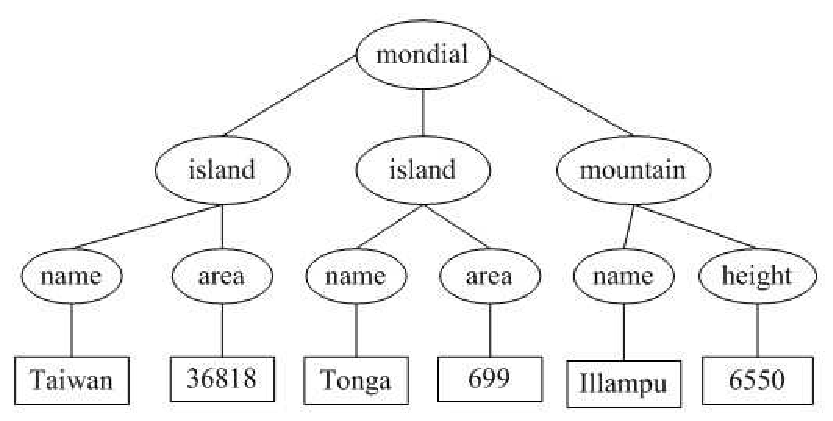
\includegraphics[width=0.4\textwidth]{XML}
\caption{树状结构}\label{fig:xml}
\vspace{\baselineskip}
\end{figure}


其插入图片的代码及其说明如下。
\vspace{1em}\noindent\hrule
\begin{verbatim}
\begin{figure}[htbp]
\centering
\includegraphics[width=0.4\textwidth]{文件名(.eps)}
\caption{标题}\label{标签名(通常为 fig:labelname)}
\vspace{\baselineskip} %表示图与正文空一行
\end{figure}
\end{verbatim}

\noindent\hrule

\begin{verbatim}
figure环境的可选参数[htbp]表示浮动图形所放置的位置,h (here)表示当前位置,t (top)表示页芯顶部,b (bottom)表示页芯底部,p (page)表示单独一页。在Word等软件中,图片通常插入到当前位置,如果当前页的剩余空间不够,图片将被移动到下一页,当前页就会出现很大的空白,其人工调整工作非常不便。由LaTeX提供的浮动图片功能,总是会按h->t->b->p的次序处理选项中的字母,自动调整图片的位置,大大减轻了工作量。
\centering命令将后续内容转换成每行皆居中的格式。
"\includegraphics"的可选参数用来设置图片插入文中的水平宽度,一般表示为正文宽度(\textwidth)的倍数。
\caption命令可选参数“标签名”为英文形式,一般不以图片或表格的数字顺序作为标签,而应包含一定的图片或表格信息,以便于文中引用(若图片、表格、公式、章节和参考文献等在文中出现的先后顺序发生了变化,其标注序号及其文中引用序号也会跟着发生变化,这一点是Word等软件所不能做到的)。另外,图题或表题并不会因为分页而与图片或表格体分置于两页,章节等各级标题也不会置于某页的最底部,LaTeX系统会自动调整它们在正文中的位置,这也是Word等软件所无法匹敌的。
\vspace将产生一定高度的竖直空白,必选参数为负值表示将后续文字位置向上提升,参数值可自行调整。em为长度单位,相当于大写字母M的宽度。\vspace{\baselineskip} 表示图与正文空一行。
引用方法:“见图~\ref{fig:figname}”、“如图~\ref{fig:figname}~所示”等。
\end{verbatim}

\noindent\hrule\vspace{1em}

若需要将~2~张及以上的图片并排插入到一行中,则需要采用\verb|minipage|环境,如图~\ref{fig:dd}~和图~\ref{fig:ds}~所示。
\begin{figure}[htbp]
\centering
\begin{minipage}{0.4\textwidth}
\centering
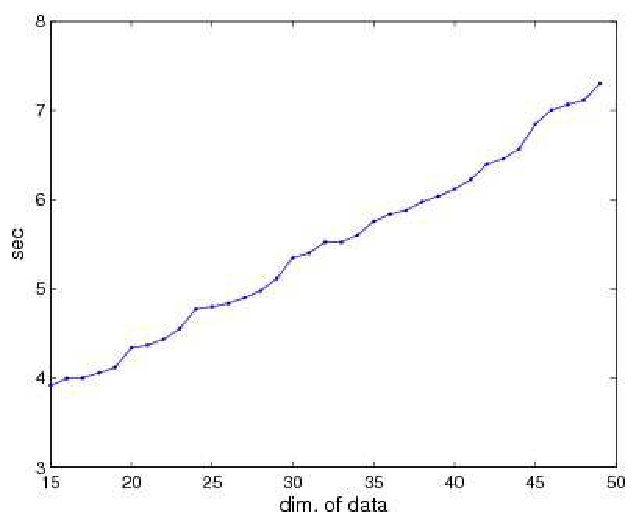
\includegraphics[width=\textwidth]{dataDimensions}
\caption{数据维数的变化}\label{fig:dd}
\end{minipage}
\begin{minipage}{0.4\textwidth}
\centering
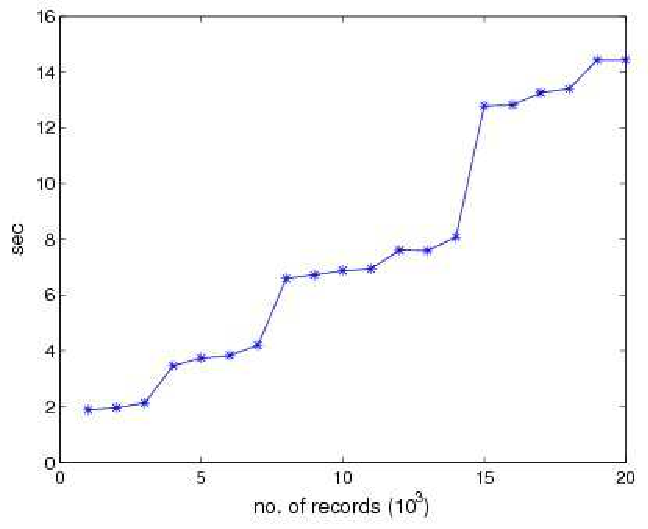
\includegraphics[width=\textwidth]{dataSize}
\caption{数据规模的变化}\label{fig:ds}
\end{minipage}
\vspace{\baselineskip}
\end{figure}

其代码如下所示。
\vspace{1em}\noindent\hrule
\begin{verbatim}
\begin{figure}[htbp]
\centering
\begin{minipage}{0.4\textwidth}
\centering
\includegraphics[width=\textwidth]{文件名}
\caption{标题}\label{fig:f1}
\end{minipage}
\begin{minipage}{0.4\textwidth}
\centering
\includegraphics[width=\textwidth]{文件名}
\caption{标题}\label{fig:f2}
\end{minipage}\vspace{\baselineskip}
\end{figure}
\end{verbatim}

\noindent\hrule

\begin{verbatim}
minipage环境的必选参数用来设置小页的宽度,若需要在一行中插入n个等宽图片,则每个小页的宽度应略小于(1/n)\textwidth。
\end{verbatim}

\noindent\hrule

\section{具有子图的图片插入方法}

图中若含有子图时,需要调用~subfigure~宏包, 如图~\ref{fig:subfig}~所示。
\begin{figure}[htbp]
  \centering
  \subfigure[Data Dimensions]{\label{fig:subfig:datadim}
                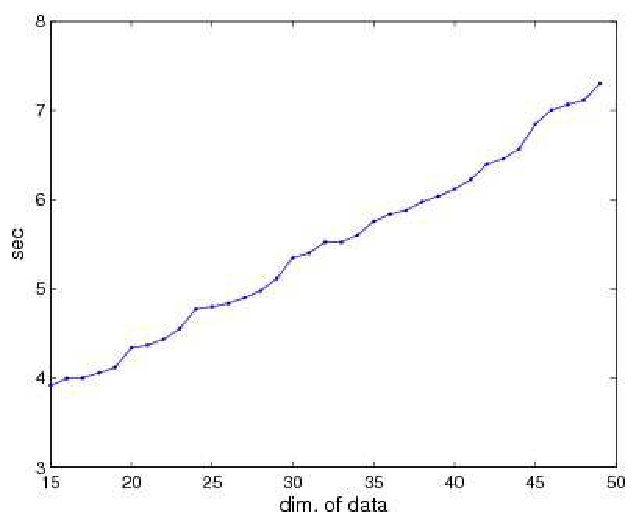
\includegraphics[width=0.4\textwidth]{dataDimensions}}
  \subfigure[Data Size]{\label{fig:subfig:datasize}
                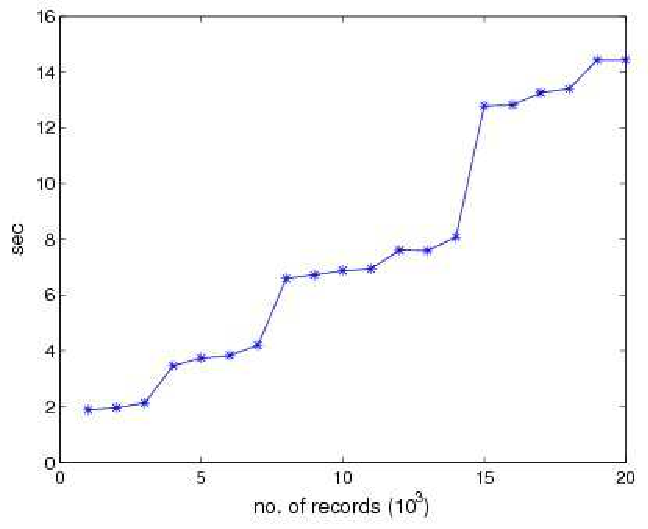
\includegraphics[width=0.4\textwidth]{dataSize}}
  \caption{Scalability of data}\label{fig:subfig}
\vspace{\baselineskip}
\end{figure}

其代码及其说明如下。
\vspace{1em}\noindent\hrule

\begin{verbatim}
\begin{figure}[htbp]
  \centering
  \subfigure[第1个子图标题]{
            \label{第1个子图标签(通常为 fig:subfig1:subsubfig1)}
            \includegraphics[width=0.4\textwidth]{文件名}}
  \subfigure[第2个子图标题]{
            \label{第2个子图标签(通常为 fig:subfig1:subsubfig2)}
            \includegraphics[width=0.4\textwidth]{文件名}}
  \caption{总标题}\label{总标签(通常为 fig:subfig1)}
\vspace{\baselineskip}
\end{figure}
\end{verbatim}

\noindent\hrule

\begin{verbatim}
子图的标签实际上可以随意设定,只要不重复就行。但为了更好的可读性,我们建议fig:subfig:subsubfig格式命名,这样我们从标签名就可以知道这是一个子图引用。
引用方法:总图的引用方法同本章第1节,子图的引用方法用\ref{fig:subfig:subsubfig}来代替。
\end{verbatim}

\noindent\hrule\vspace{1em}

子图的引用示例:如图~\ref{fig:subfig:datadim}~和图~\ref{fig:subfig:datasize}~所示。

若想获得插图方法的更多信息,参见网络上的~\href{ftp://ftp.tex.ac.uk/tex-archive/info/epslatex.pdf}{Using Imported Graphics in \LaTeX and pdf\LaTeX}~文档。 
%%% !Mode:: "TeX:UTF-8"

\chapter{表格的绘制方法}
\section{研究生毕业设计论文的绘表规范}

表应有自明性。表格不加左、右边线。表的编排建议采用国际通行的三线表。表内中文书写使用宋体五号字。

每个表格之上均应有表题(由表序和表名组成)。表序一般按章编排,如第~1~章第一个插表的序号为“表~1-1”等。表序与表名之间空两格,
表名使用中文五号字,居中。表名中不允许使用标点符号,表名后不加标点。
表头设计应简单明了,尽量不用斜线。表头中可采用化学,物理量等专业符号。

全表如用同一单位,则将单位符号移至表头右上角,加圆括号。
表中数据应准确无误,书写清楚。数字空缺的格内加横线“-”(占~2~个数字宽度)。表内文字或数字上、下或左、右相同时,
采用通栏处理方式,不允许用“〃”、“同上”之类的写法。

表内文字使用宋体五号字,垂直居中书写,起行空一格、转行顶格、句末不加标点。
如某个表需要转页接排,在随后的各页上应重复表的编号。编号后加“(续表)”,表题可省略。续表应重复表头。
表格绘制完成之后,与正文空一行。

\section{普通表格的绘制方法}

表格应具有三线表格式,因此需要调用~booktabs~宏包,其标准格式如表~\ref{tab:table1}~所示。
\begin{table}[htbp]
\caption{符合本科生毕业论文绘图规范的表格}\label{tab:table1}
\vspace{0.5em}\centering\wuhao
\begin{tabular}{ccccc}
\toprule[1.5pt]
$D$(in) & $P_u$(lbs) & $u_u$(in) & $\beta$ & $G_f$(psi.in)\\
\midrule[1pt]
 5 & 269.8 & 0.000674 & 1.79 & 0.04089\\
10 & 421.0 & 0.001035 & 3.59 & 0.04089\\
20 & 640.2 & 0.001565 & 7.18 & 0.04089\\
 5 & 269.8 & 0.000674 & 1.79 & 0.04089\\
10 & 421.0 & 0.001035 & 3.59 & 0.04089\\
20 & 640.2 & 0.001565 & 7.18 & 0.04089\\
 5 & 269.8 & 0.000674 & 1.79 & 0.04089\\
10 & 421.0 & 0.001035 & 3.59 & 0.04089\\
20 & 640.2 & 0.001565 & 7.18 & 0.04089\\
 5 & 269.8 & 0.000674 & 1.79 & 0.04089\\
10 & 421.0 & 0.001035 & 3.59 & 0.04089\\
20 & 640.2 & 0.001565 & 7.18 & 0.04089\\
\bottomrule[1.5pt]
\end{tabular}
\vspace{\baselineskip}
\end{table}

其绘制表格的代码及其说明如下。
\vspace{1em}\noindent\hrule

\begin{verbatim}
\begin{table}[htbp]
\caption{表标题}\label{标签名(通常为 tab:tablename)}
\vspace{0.5em}\centering\wuhao
\begin{tabular}{cc...c}
\toprule[1.5pt]
表头第1个格   & 表头第2个格   & ... & 表头第n个格  \\
\midrule[1pt]
表中数据(1,1) & 表中数据(1,2) & ... & 表中数据(1,n)\\
表中数据(2,1) & 表中数据(2,2) & ... & 表中数据(2,n)\\
表中数据(3,1) & 表中数据(3,2) & ... & 表中数据(3,n)\\
表中数据(4,1) & 表中数据(4,2) & ... & 表中数据(4,n)\\
...................................................\\
表中数据(m,1) & 表中数据(m,2) & ... & 表中数据(m,n)\\
\bottomrule[1.5pt]
\end{tabular}
\vspace{\baselineskip}
\end{table}
\end{verbatim}

\noindent\hrule

\begin{verbatim}
table环境是一个将表格嵌入文本的浮动环境。
\wuhao命令将表格的字号设置为五号字(10.5pt),在绘制表格结束退出时,不需要将字号再改回为\xiaosi,正文字号默认为小四号字(12pt)。
tabular环境的必选参数由每列对应一个格式字符所组成:c表示居中,l表示左对齐,r表示右对齐,其总个数应与表的列数相同。此外,@{文本}可以出现在任意两个上述的列格式之间,其中的文本将被插入每一行的同一位置。表格的各行以\\分隔,同一行的各列则以&分隔。
\toprule、\midrule和\bottomrule三个命令是由booktabs宏包提供的,其中\toprule和\bottomrule分别用来绘制表格的第一条(表格最顶部)和第三条(表格最底部)水平线,\midrule用来绘制第二条(表头之下)水平线,且第一条和第三条水平线的线宽为1.5pt,第二条水平线的线宽为1pt。
引用方法:“如表~\ref{tab:tablename}~所示”。
\end{verbatim}

\noindent\hrule

\section{长表格的绘制方法}

长表格是当表格在当前页排不下而需要转页接排的情况下所采用的一种表格环境。若长表格仍按照普通表格的绘制方法来获得,
其所使用的\verb|table|浮动环境无法实现表格的换页接排功能,表格下方过长部分会排在表格第1页的页脚以下。为了能够实现长表格的转页接排功能,
需要调用~longtable~宏包,由于长表格是跨页的文本内容,因此只需要单独的\verb|longtable|环境,所绘制的长表格的格式如表~\ref{tab:table2}~所示。

此长表格~\ref{tab:table2}~第~2~页的标题“编号(续表)”和表头是通过代码自动添加上去的,无需人工添加,若表格在页面中的竖直位置发生了变化,长表格在第~2~页
及之后各页的标题和表头位置能够始终处于各页的最顶部,也无需人工调整,\LaTeX~系统的这一优点是~Word~等软件所无法企及的。

下段内容是为了让下面的长表格分居两页,看到表标题“编号(续表)”的效果。摘录于《你若安好,便是晴天 -- 林徽因传》片段:

她叫林徽因,出生于杭州,是许多人梦中期待的白莲。她在雨雾之都伦敦,发生过一场空前绝后的康桥之恋。她爱过三个男子,爱得清醒,也爱得平静。徐志摩为她徜徉在康桥,深情地等待一场旧梦可以归来。梁思成与她携手走过千山万水,为完成使命而相约白头。金岳霖为她终身不娶,痴心不改地守候一世。可她懂得人生飘忽不定,要学会随遇而安。
真正的平静,不是避开车马喧嚣,而是在心中修篱种菊。尽管如流往事,每一天都涛声依旧,只要我们消除执念,便可寂静安然。愿每个人在纷呈世相中不会迷失荒径,可以端坐磐石上,醉倒落花前。
如果可以,请让我预支一段如莲的时光,哪怕将来某一天加倍偿还。这个雨季会在何时停歇,无从知晓。但我知道,你若安好,便是晴天。					
\wuhao\begin{longtable}{ccc}
\caption{天津大学各学院名称一览}\label{tab:table2}
 \vspace{0.5em}\\
\toprule[1.5pt] 学院名称 & 网址 & 联系电话  \\ \midrule[1pt]
\endfirsthead
\multicolumn{3}{c}{表~\thetable(续表)}\vspace{0.5em}\\
\toprule[1.5pt] 学院名称 & 网址 & 联系电话  \\ \midrule[1pt]
\endhead
\bottomrule[1.5pt]
\endfoot
机械工程学院& \url{http://tdjxxy.tju.edu.cn/}& 87401979\\
精密仪器与光电子工程学院&  \url{http://www2.tju.edu.cn/colleges/precision/cn/}& 27404775\\
电子信息工程学院& \url{http://www.tju.edu.cn/seie}& 27406956\\
电气与自动化工程学院& \url{http://www2.tju.edu.cn/colleges/automate/}& 27405477\\
建筑工程学院& \url{http://www2.tju.edu.cn/colleges/civil/}& 27404072\\
化工学院& \url{http://chemeng.tju.edu.cn/}& 27403389\\
材料科学与工程学院& \url{http://mse.tju.edu.cn}& 27406693 \\
建筑学院& \url{http://hgw022072.chinaw3.com/}& 27402724-2111\\
求是学部\\
管理与经济学部&	\url{ http://sm.tju.edu.cn}& 27403423\\
理学院& \url{ http://www.tju.edu.cn/science/}& 27404118\\
文法学院& \url{ http://www2.tju.edu.cn/colleges/sociology/new/}& 27403691\\
软件学院& \url{http://scs.tju.edu.cn}& 87401540\\
计算机科学与技术学院& \url{http://cs.tju.edu.cn/}& 27406538\\
马克思主义学院& \url{http://www2.tju.edu.cn/colleges/marxism/}& 27405348\\
环境科学与工程学院& \url{http://www.tju.edu.cn/see}& 87402072\\
药物科学与技术学院& \url{http://www2.tju.edu.cn/colleges/pharmtier/}& 87401830\\
教育学院& \url{http://soe.tju.edu.cn/}& 27401028\\
职业技术教育学院& \url{http://202.113.0.248:8888}\\
继续教育学院& \url{http://aectu.tju.edu.cn/}& 27406298\\
仁爱学院& \url{http://www.tjrac.edu.cn/}& 68579990\\
农业与生物工程学院& \url{http://202.113.13.169/site/nongxueyuan/}& 87402171\\
国际教育学院 & \url{http://www.ietju.com/}& 27406147\\
网络教育学院 & \url{http://www.etju.com/}& 27426952 \\

\end{longtable}\xiaosi
\vspace{\baselineskip}

绘制长表格的代码及其说明如下。
\vspace{1em}\noindent\hrule

\begin{verbatim}
\wuhao\begin{longtable}{cc...c}
\caption{表标题}\label{标签名(通常为 tab:tablename)}\\
\toprule[1.5pt] 表头第1个格 & 表头第2个格 & ... & 表头第n个格\\ \midrule[1pt]
\endfirsthead
\multicolumn{n}{c}{表~\thetable(续表)}\vspace{0.5em}\\
\toprule[1.5pt] 表头第1个格 & 表头第2个格 & ... & 表头第n个格\\ \midrule[1pt]
\endhead
\bottomrule[1.5pt]
\endfoot
表中数据(1,1) & 表中数据(1,2) & ... & 表中数据(1,n)\\
表中数据(2,1) & 表中数据(2,2) & ... & 表中数据(2,n)\\
...................................................\\
表中数据(m,1) & 表中数据(m,2) & ... & 表中数据(m,n)\\
\end{longtable}\xiaosi
\end{verbatim}

\noindent\hrule
\begin{verbatim}
在绘制长表格的前面留出一个空白行,并在第2行的一开始全局定义长表格的字号为五号字,这样能够保证长表格之前段落的行距保持不变。
在绘制长表格结束后,需要\xiaosi命令重新将字号改为小四号字。
\endhead之前的文字描述的是第2页及其之后各页的标题或表头;
\endfirsthead之前的文字描述的是第1页的标题和表头,若无此命令,则第1页的表头和标题由\endhead命令确定;
同理,\endfoot之前的文字描述的是除最后一页之外每页的表格底部内容;
\endlastfoot之前的文字描述的是最后一页的表格底部内容,若无此命令,
则最后一页的表格底部内容由\endfoot命令确定;由于规范中长表格每页底部内容均相同(水平粗线),因此模板中没有用到\endlastfoot命令。
\end{verbatim}

\noindent\hrule
\section{列宽可调表格的绘制方法}
论文中能用到列宽可调表格的情况共有两种:一种是当插入的表格某一单元格内容过长以至于一行放不下的情况,
另一种是当对公式中首次出现的物理量符号进行注释的情况。这两种情况都需要调用~tabularx~宏包。下面将分别对这两种情况下可调表格的绘制方法进行阐述。
\subsection{表格内某单元格内容过长的情况}

首先给出这种情况下的一个例子如表~\ref{tab:table3}~所示。
\begin{table}[htbp]
\caption{最小的三个正整数的英文表示法}\label{tab:table3}
\vspace{0.5em}\wuhao
\begin{tabularx}{\textwidth}{llX}
\toprule[1.5pt]
Value & Name & Alternate names, and names for sets of the given size\\\midrule[1pt]
1 & One & ace, single, singleton, unary, unit, unity\\
2 & Two & binary, brace, couple, couplet, distich, deuce, double, doubleton, duad, duality, duet, duo, dyad, pair, snake eyes, span, twain, twosome, yoke\\
3 & Three & deuce-ace, leash, set, tercet, ternary, ternion, terzetto, threesome, tierce, trey, triad, trine, trinity, trio, triplet, troika, hat-trick\\\bottomrule[1.5pt]
\end{tabularx}
\vspace{\baselineskip}
\end{table}
绘制这种表格的代码及其说明如下。
\vspace{1em}\noindent\hrule
\begin{verbatim}
\begin{table}[htbp]
\caption{表标题}\label{标签名(通常为 tab:tablename)}
\vspace{0.5em}\wuhao
\begin{tabularx}{\textwidth}{l...X...l}
\toprule[1.5pt]
表头第1个格   & ... & 表头第X个格   & ... & 表头第n个格  \\
\midrule[1pt]
表中数据(1,1) & ... & 表中数据(1,X) & ... & 表中数据(1,n)\\
表中数据(2,1) & ... & 表中数据(2,X) & ... & 表中数据(2,n)\\
.........................................................\\
表中数据(m,1) & ... & 表中数据(m,X) & ... & 表中数据(m,n)\\
\bottomrule[1.5pt]
\end{tabularx}
\vspace{\baselineskip}
\end{table}
\end{verbatim}

\noindent\hrule
\begin{verbatim}
tabularx环境共有两个必选参数:第1个参数用来确定表格的总宽度,这里取为排版表格能达到的最大宽度——正文宽度\textwidth;第2个参数用来确定每列格式,其中标为X的项表示该列的宽度可调,其宽度值由表格总宽度确定。
标为X的列一般选为单元格内容过长而无法置于一行的列,这样使得该列内容能够根据表格总宽度自动分行。若列格式中存在不止一个X项,则这些标为X的列的列宽相同,因此,一般不将内容较短的列设为X。
标为X的列均为左对齐,因此其余列一般选为l(左对齐),这样可使得表格美观,但也可以选为c或r。
\end{verbatim}

\noindent\hrule
\subsection{对物理量符号进行注释的情况}
为使得对公式中物理量符号注释的转行与破折号“———”后第一个字对齐,此处最好采用表格环境。此表格无任何线条,左对齐,
且在破折号处对齐,一共有“式中”二字、物理量符号和注释三列,表格的总宽度可选为文本宽度,因此应该采用\verb|tabularx|环境。
由\verb|tabularx|环境生成的对公式中物理量符号进行注释的公式如式(\ref{eq:1})所示。
%\vspace*{10pt}

\begin{equation}\label{eq:1}
\ddot{\boldsymbol{\rho}}-\frac{\mu}{R_{t}^{3}}\left(3\mathbf{R_{t}}\frac{\mathbf{R_{t}\rho}}{R_{t}^{2}}-\boldsymbol{\rho}\right)=\mathbf{a}
\end{equation}

\begin{tabularx}{\textwidth}{@{}l@{\quad}r@{———}X@{}}
式中& $\bm{\rho}$ &追踪飞行器与目标飞行器之间的相对位置矢量;\\
&  $\bm{\ddot{\rho}}$&追踪飞行器与目标飞行器之间的相对加速度;\\
&  $\mathbf{a}$   &推力所产生的加速度;\\
&  $\mathbf{R_t}$ & 目标飞行器在惯性坐标系中的位置矢量;\\
&  $\omega_{t}$ & 目标飞行器的轨道角速度;\\
&  $\mathbf{g}$ & 重力加速度,$=\frac{\mu}{R_{t}^{3}}\left(
3\mathbf{R_{t}}\frac{\mathbf{R_{t}\rho}}{R_{t}^{2}}-\bm{\rho}\right)=\omega_{t}^{2}\frac{R_{t}}{p}\left(
3\mathbf{R_{t}}\frac{\mathbf{R_{t}\rho}}{R_{t}^{2}}-\bm{\rho}\right)$,这里~$p$~是目标飞行器的轨道半通径。
\end{tabularx}
\vspace{\wordsep}

其中生成注释部分的代码及其说明如下。

\vspace{1em}\noindent\hrule

\begin{verbatim}
\begin{tabularx}{\textwidth}{@{}l@{\quad}r@{— — —}X@{}}
式中 & symbol-1 & symbol-1的注释内容;\\
     & symbol-2 & symbol-2的注释内容;\\
     .............................;\\
     & symbol-m & symbol-m的注释内容。
\end{tabularx}\vspace{\wordsep}
\end{verbatim}

\noindent\hrule

\begin{verbatim}
tabularx环境的第1个参数选为正文宽度,第2个参数里面各个符号的意义为:
    第1个@{}表示在“式中”二字左侧不插入任何文本,“式中”二字能够在正文中左对齐,若无此项,则“式中”二字左侧会留出一定的空白;
    @{\quad}表示在“式中”和物理量符号间插入一个空铅宽度的空白;
    @{— — —}实现插入破折号的功能,它由三个1/2的中文破折号构成;
    第2个@{}表示在注释内容靠近正文右边界的地方能够实现右对齐。
\end{verbatim}

\noindent\hrule\vspace{1em}

由此方法生成的注释内容应紧邻待注释公式并置于其下方,因此不能将代码放入\verb|table|浮动环境中。但此方法不能实现自动转页接排,
可能会在当前页剩余空间不够时,全部移动到下一页而导致当前页出现很大空白。因此在需要转页处理时,还请您手动将需要转页的代码放入一个
新的\verb|tabularx|环境中,将原来的一个\verb|tabularx|环境拆分为两个\verb|tabularx|环境。

若想获得绘制表格的更多信息,参见网络上的~\href{http://www.tug.org/pracjourn/2007-1/mori/}{Tables in \LaTeXe: Packages and Methods}~文档。


%%% !Mode:: "TeX:UTF-8"

\chapter{数学公式的输入方法}
\section{研究生毕业设计论文的公式规范}

论文中的公式应另起行,原则上应居中书写,与周围文字留有足够的空间区分开。
若公式前有文字(如“解”、“假定”等),文字空两格写,公式仍居中写。公式末不加标点。

公式应标注序号,并将序号置于括号内。 公式序号按章编排,如第~1~章第一个公式序号为“(1-1)”。公式的序号右端对齐。

公式较长时最好在等号“=”处转行,如难实现,则可在~$+$、$-$、$\times$、$\div$~运算符号处转行,转行时运算符号仅书写于转行式前,不重复书写。

文中引用公式时,一般用“见式~(1-1)”或“由公式~(1-1)”。

公式中用斜线表示“除”的关系时应采用括号,以免含糊不清,如~$a/(b\cos x)$。通常“乘”的关系在前,如~$a\cos x/b$而不写成~$(a/b)\cos x$。

不能用文字形式表示等式,如:$\textnormal{刚度}=\frac{{\textnormal{受力}}}{{\textnormal{受力方向的位移}}}$。

对于数学公式的输入方法,网络上有一个比较全面权威的文档\textbf{~\href{http://tug.ctan.org/cgi-bin/ctanPackageInformation.py?id=voss-mathmode}{Math mode}}~请大家事先大概浏览一下。下面将对学位论文中主要用到的数学公式排版形式进行阐述。

\section{生成~\LaTeX~数学公式的两种方法}
对于先前没有接触过~\LaTeX~的人来说,编写~\LaTeX~数学公式是一件很繁琐的事,尤其是对复杂的数学公式来说,更可以说是一件难以完成的任务。
实际上,生成~\LaTeX~数学公式有两种较为简便的方法,一种是基于~MathType~数学公式编辑器的方法,另一种是基于~MATLAB~商业数学软件的方法,
下面将分别对这两种数学公式的生成方法作一下简单介绍。

\subsection{基于~MathType~软件的数学公式生成方法}
MathType~是一款功能强大的数学公式编辑器软件,能够用来在文本环境中插入~Windows OLE~图形格式的复杂数学公式,所以应用比较普遍。但此软件只有~30~天的试用期,之后若再继续使用则需要付费购买才行。网络上有很多破解版的~MathType~软件可供下载免费使用,
笔者推荐下载安装版本号在~6.5~之上的中文破解版。

在安装好~MathType~之后,若在输入窗口中编写数学公式,复制到剪贴板上的仍然是图形格式的对象。
若希望得到可插入到~\LaTeX~编辑器中的文本格式对象,则需要对~MathType~软件做一下简单的设置:在~MathType~最上排的按钮中依次选择“参数选项
$\to$转换”,在弹出的对话窗中选中“转换到其它语言(文字):”,在转换下拉框中选择“Tex~--~--~LaTeX 2.09 and later”,并将对话框最下方的两个复选框全部勾掉,点击确定,这样,再从输入窗口中复制出来的对象就是文本格式的了,就可以直接将其粘贴到~\LaTeX~
编辑器中了。按照这种方法生成的数学公式两端分别有标记\verb|\[|和标记\verb|\]|,在这两个标记之间才是真正的数学公式代码。

若希望从~MathType~输入窗口中复制出来的对象为图形格式,则只需再选中“公示对象(Windows OLE~图形)”即可。

\subsection{基于~MATLAB~软件的数学公式生成方法}

MATLAB~是矩阵实验室(Matrix Laboratory)的简称,是美国~MathWorks~公司出品的商业数学软件。它是当今科研领域最常用的应用软件之一,
具有强大的矩阵计算、符号运算和数据可视化功能,是一种简单易用、可扩展的系统开发环境和平台。

MATLAB~中提供了一个~latex~函数,它可将符号表达式转化为~\LaTeX~数学公式的形式。其语法形式为~latex(s),其中,~s~为符号表达式,
之后再将~latex~函数的运算结果直接粘贴到~\LaTeX~编辑器中。从~\LaTeX~数学公式中可以发现,其中可能包含如下符号组合:

\begin{verbatim*}
\qquad=两个空铅(quad)宽度
\quad=一个空铅宽度
\;=5/18空铅宽度
\:=4/18空铅宽度
\,=3/18空铅宽度
\!=-3/18空铅宽度
\ =一个空格
\end{verbatim*}

所以最好将上述符号组合从数学公式中删除,从而使数学公式显得匀称美观。

对于~Word~等软件的使用者来说,在我们通过~MATLAB~运算得到符号表达式形式的运算结果时,在~Word~中插入运算结果需要借助于~MathType~软件,
通过在~MathType~中输入和~MATLAB~运算结果相对应的数学表达形式,之后再将~MathType~数学表达式转换为图形格式粘贴到~Word~中。实际上,
也可以将~MATLAB~中采用~latex~函数运行的结果直接粘贴到~MathType~中,再继续上述步骤,这样可以大大节省输入公式所需要的时间。
此方法在~MathType~6.5c~上验证通过,若您粘入到~MathType~中的仍然为从~MATLAB~中导入的代码,请您更新~MathType~软件。

\section{数学字体}
在数学模式下,常用的数学字体命令有如下几种:

\begin{verbatim}
\mathnormal或无命令 用数学字体打印文本;
\mathit             用斜体(\itshape)打印文本;
\mathbf             用粗体(\bfseries)打印文本;
\mathrm             用罗马体(\rmfamily)打印文本;
\mathsf             用无衬线字体(\sffamily)打印文本;
\mathtt             用打印机字体(\ttfamily)打印文本;
\mathcal            用书写体打印文本;
\end{verbatim}

在学位论文撰写中,只需要用到上面提到的~\verb|\mathit|、\verb|\mathbf|~和~\verb|\mathrm|~命令。若要得到~Times New Roman~的数学字体,则需要调用~txfonts~宏包(此宏包实际上采用的是~Nimbus Roman No9 L~字体,
它是开源系统中使用的免费字体,其字符字体与~Times New Roman~字体几乎完全相同);若要得到粗体数学字体,则需要调用~bm~宏包。表~\ref{tab:fonts}~中分别列出了得到阿拉伯数字、拉丁字母和希腊字母
各种数学字体的命令。

\begin{table}[htbp]
\caption{常用数学字体命令一览}\label{tab:fonts}
\vspace{0.5em}\centering\wuhao
\begin{tabular}{llll}
\toprule
 & 阿拉伯数字\&大写希腊字母 & 大小写拉丁字母 & 小写希腊字母  \\
\midrule
斜体 & \verb|\mathit{}| & \verb|无命令| & \verb|无命令|\\
粗斜体 & \verb|\bm{\mathit{}}| & \verb|\bm{}| & \verb|\bm{}|\\
直立体 & \verb|无命令| & \verb|\mathrm{}| & \verb|字母后加up|\\
粗体 & \verb|\mathbf{}或\bm{}| & \verb|\mathbf{}| & \verb|\bm{字母后加up}|\\
\bottomrule
\end{tabular}
\vspace{\baselineskip}
\end{table}

\noindent 下面列出了一些应采用直立数学字体的数学常数和数学符号。

\vspace{-0.5em}\begin{center}\begin{tabularx}{0.7\textwidth}{XX}
$\mathrm{d}$、 $\mathrm{D}$、 $\mathrm{p}$~———微分算子 & $\mathrm{e}$~———自然对数之底数\\
$\mathrm{i}$、 $\mathrm{j}$~———虚数单位 & $\piup$———圆周率\\
\end{tabularx}\end{center}

\section{行内公式}
出现在正文一行之内的公式称为行内公式,例如~$f(x)=\int_{a}^{b}\frac{\sin{x}}{x}\mathrm{d}x$。对于非矩阵和非多行形式的行内公式,一般不会使得行距发生变化,而~Word~等软件却会根据行内公式的竖直距离而自动调节行距,如图~\ref{fig:hangju}~所示。

\begin{figure}[htbp]
\centering
\subfigure[由~\LaTeX~系统生成的行内公式]{\label{fig:subfig:latex}
                \fbox{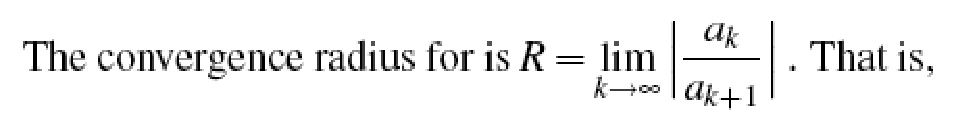
\includegraphics[width=0.55\textwidth]{latex}}}
\subfigure[由~Word软件生成的~.doc~格式行内公式]{\label{fig:subfig:word}
                \fbox{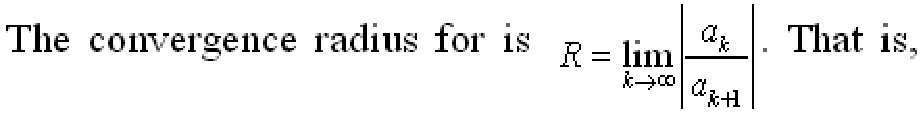
\includegraphics[width=0.55\textwidth]{word}}}
\subfigure[由~Word软件生成的~.pdf~格式行内公式]{\label{fig:subfig:pdf}
                \fbox{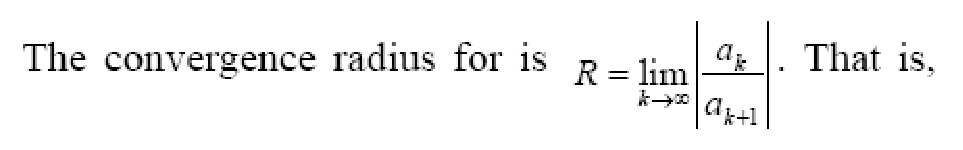
\includegraphics[width=0.55\textwidth]{pdf}}}

\caption{由~\LaTeX~和~Word~生成的~3~种行内公式屏显效果}\label{fig:hangju}
\vspace{-1em}
\end{figure}

这三幅图分别为~\LaTeX~和~Word~生成的行内公式屏显效果,从图中可看出,在~\LaTeX~文本含有公式的行内,在正文与公式之间对接工整,行距不变;而在~Word~文本含有公式的行内,在正文与公式之间对接不齐,行距变大。因此从这一点来说,
\LaTeX~系统在数学公式的排版上具有很大优势。

\LaTeX~提供的行内公式最简单、最有效的方法是采用~\TeX~本来的标记———开始和结束标记都写作~\$,例如本段开始的例子可由下面的输入得到。
\verb|$f(x)=\int_{a}^{b}\frac{\sin{x}}{x}\mathrm{d}x$|

\section{行间公式}
位于两行之间的公式称为行间公式,每个公式都是一个单独的段落,例如
\[\int_a^b{f\left(x\right)\mathrm{d}x}=\lim_{\left\|\Delta{x_i}\right\|\to 0}\sum_i{f\left(\xi_i\right)\Delta{x_i}}\]
除人工编号外,\LaTeX~各种类型行间公式的标记见表~\ref{tab:eqtag}。
\begin{table}[htbp]
\caption{各种类型行间公式的标记}\label{tab:eqtag}
\vspace{0.5em}\centering\wuhao
\begin{tabularx}{\textwidth}{cll}
\toprule
& 无编号 & 自动编号\\
\midrule
单行公式& \verb|\begin{displaymath}... \end{displaymath}|& \verb|\begin{equation}... \end{equation}|\\
        & 或~\verb|\[...\]| & \\
多行公式& \verb|\begin{eqnarray*}... \end{eqnarray*}|& \verb|\begin{eqnarray}... \end{eqnarray}|\\
\bottomrule
\end{tabularx}
\end{table}

另外,在自动编号的某行公式行尾添加标签~\verb|\nonumber|,可将该行转换为无编号形式。

行间多行公式需采用~\verb|eqnarray|~或~\verb|eqnarray*|~环境,它默认是一个列格式为~\verb|rcl|~的~3~列矩阵,并且中间列的字号要小一些,因此通常只将需要对齐的运算符号(通常为等号“=”)置于中间列。

\section{可自动调整大小的定界符}
若在左右两个定界符之前分别添加命令~\verb|\left|~和~\verb|\right|,则定界符可根据所包围公式大小自动调整其尺寸,这可从式(\ref{nodelimiter})和式(\ref{delimiter})中看出。
\begin{equation}\label{nodelimiter}
(\sum_{k=\frac12}^{N^2})
\end{equation}
\begin{equation}\label{delimiter}
\left(\sum_{k=\frac12}^{N^2}\right)
\end{equation}
式(\ref{nodelimiter})和式(\ref{delimiter})是在~\LaTeX~中分别输入如下代码得到的。
\begin{verbatim}
(\sum_{k=\frac12}^{N^2})
\left(\sum_{k=\frac12}^{N^2}\right)
\end{verbatim}
\verb|\left|~和~\verb|\right|~总是成对出现的,若只需在公式一侧有可自动调整大小的定界符,则只要用“.”代替另一侧那个无需打印出来的定界符即可。

若想获得关于此部分内容的更多信息,可参见~\href{http://tug.ctan.org/cgi-bin/ctanPackageInformation.py?id=voss-mathmode}{Math mode}~文档的第~8~章“Brackets, braces and parentheses”。

\section{数学重音符号}
数学重音符号通常用来区分同一字母表示的不同变量,输入方法如下(需要调用~\verb|amsmath|~宏包):

\vspace{0.5em}\noindent\wuhao\begin{tabularx}{\textwidth}{Xc|Xc|Xc}
 \verb|\acute| & $\acute{a}$ & \verb|\mathring| & $\mathring{a}$ & \verb|\underbrace| & $\underbrace{a}$ \\
 \verb|\bar| & $\bar{a}$ & \verb|\overbrace| & $\overbrace{a}$ & \verb|\underleftarrow| & $\underleftarrow{a}$ \\
 \verb|\breve| & $\breve{a}$ & \verb|\overleftarrow| & $\overleftarrow{a}$ & \verb|\underleftrightarrow| & $\underleftrightarrow{a}$ \\
 \verb|\check| & $\check{a}$ & \verb|\overleftrightarrow| & $\overleftrightarrow{a}$ & \verb|\underline| & $\underline{a}$ \\
 \verb|\dddot| & $\dddot{a}$ & \verb|\overline| & $\overline{a}$ & \verb|\underrightarrow| & $\underrightarrow{a}$ \\
 \verb|\ddot| & $\ddot{a}$ & \verb|\overrightarrow| & $\overrightarrow{a}$ & \verb|\vec| & $\vec{a}$ \\
 \verb|\dot| & $\dot{a}$ & \verb|\tilde| & $\tilde{a}$ & \verb|\widehat| & $\widehat{a}$ \\
 \verb|\grave| & $\grave{a}$ & \verb|\underbar| & $\underbar{a}$ & \verb|\widetilde| & $\widetilde{a}$ \\
 \verb|\hat| & $\hat{a}$
\end{tabularx}\vspace{0.5em}
\xiaosi 当需要在字母~$i$~和~$j$~的上方添加重音符号时,为了去掉这两个字母顶上的小点,这两个字母应该分别改用~\verb|\imath|~和~\verb|\jmath|。

如果遇到某些符号不知道该采用什么命令能输出它时,则可通过~\href{http://detexify.kirelabs.org/classify.html}{Detexify$^2$~网站}来获取符号命令。若用鼠标左键在此网页的方框区域内画出你所要找的符号形状,则会在网页右方列出和你所画符号形状相近的~5~个符号及其相对应的~\LaTeX~输入命令。若所列出的符号中不包括你所要找的符号,还可通过点击“Select from the complete list!”的链接以得分从低到高的顺序列出所有符号及其相对应的~\LaTeX~输入命令。

最后,建议大家还以~\href{http://tug.ctan.org/cgi-bin/ctanPackageInformation.py?id=voss-mathmode}{Math mode}~这篇~pdf~文档作为主要参考。若要获得最为标准、美观的数学公式排版形式,可以查查文档中是否有和你所要的排版形式相同或相近的代码段,通过修改代码段以获得你所要的数学公式排版形式。


%%% !Mode:: "TeX:UTF-8"

\chapter{罗列和定理环境使用方法}

\section{单层罗列环境}
天津大学学位论文一般可采用两种罗列环境:一种是并列条目有同样标签的~\verb|itemize|~罗列环境,另一种是具有自动排序编号符号的~\verb|enumerate|~罗列环境。这两种罗列环境的样式参数可参考图~\ref{fig:list}。
\begin{figure}[htbp]
\centering
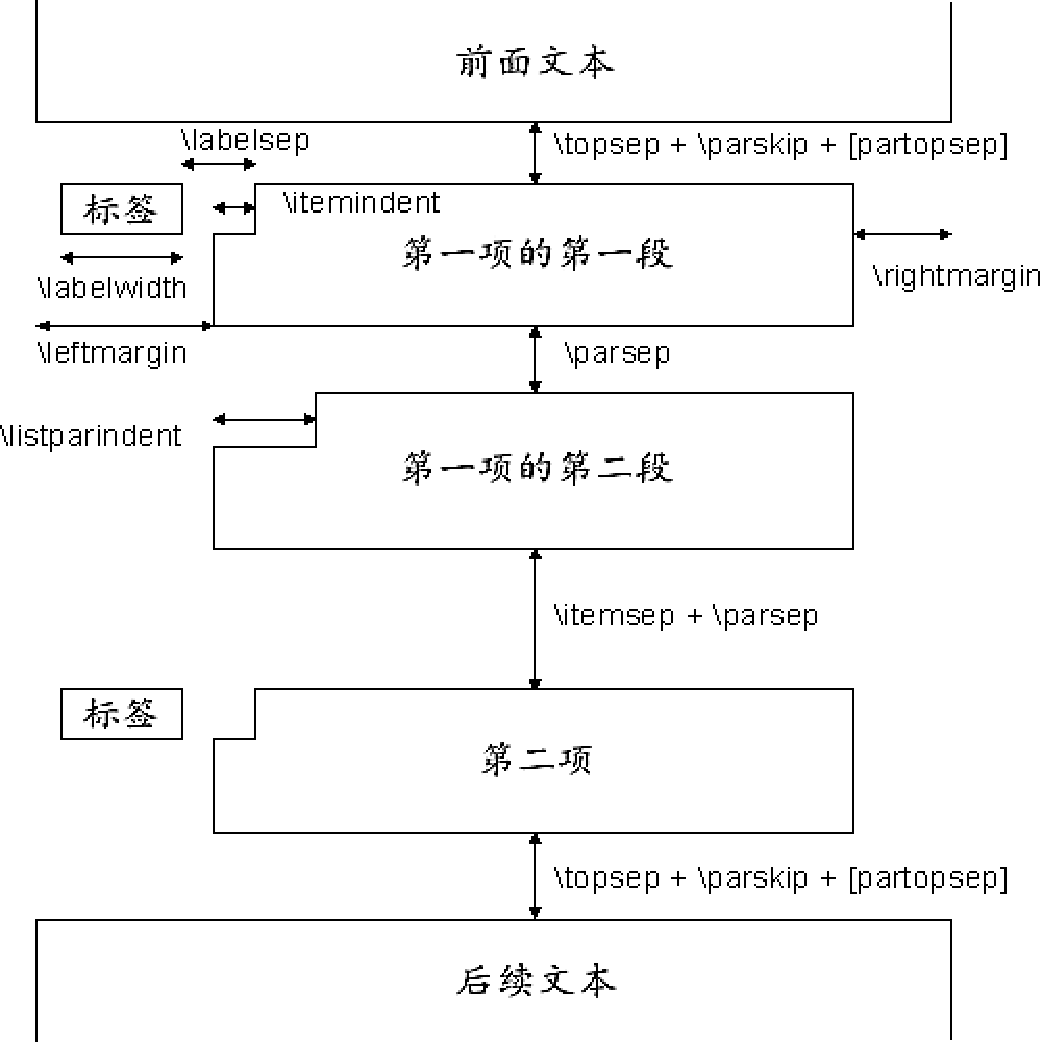
\includegraphics[width = 0.6\textwidth]{list}
\caption{罗列环境参数示意图}\label{fig:list}\vspace{-1em}
\end{figure}

通过调用~enumitem~宏包可以很方便地控制罗列环境的布局,其~format.tex~文件中的~\verb|\setitemize|~和~\verb|\setenumerate|~命令分别用来设置~\verb|itemize|~和~\verb|enumerate|~环境的样式参数。采用~\verb|itemize|~单层罗列环境的排版形式如下:

\begin{itemize}
\item 第一个条目文本内容
\item 第二个条目文本内容
\item 第三个条目文本内容
\end{itemize}

其代码如下

\begin{verbatim}
\begin{itemize}
  \item 第一个条目文本内容
  \item 第二个条目文本内容
  ...
  \item 第三个条目文本内容
\end{itemize}
\end{verbatim}

采用~\verb|enumerate|~单层罗列环境的排版形式如下:

\begin{enumerate}
\item 第一个条目文本内容
\item 第二个条目文本内容
\item 第三个条目文本内容
\end{enumerate}

其代码如下

\begin{verbatim}
\begin{enumerate}
  \item 第一个条目文本内容
  \item 第二个条目文本内容
  ...
  \item 第三个条目文本内容
\end{enumerate}
\end{verbatim}



\section{定理环境}

\begin{definition}[谱半径]\label{def:def1}
  称~$n$~阶方阵~$\mathbf{A}$~的全体特征值~$\lambda_1,\cdots,\lambda_n$~组成的集合为~$\mathbf{A}$~的谱,称
  $$\rho(\mathbf{A})=\max{\{|\lambda_1|,\cdots,|\lambda_n|\}}$$
\end{definition}
\begin{theorem}[相似充要条件]\label{lemma:l1}
  方阵$A$和$B$相似的充要条件是:~$A$~和~$B$~有全同的不变因子。
\end{theorem}
\begin{corollary}[推论1]\label{cor:cor1}
在赋范空间~$(X,\|\cdot\|)$~上定义~$d(x,y)=\|x-y\|$, 对任意~$x,y\in X$,~则~$(X,d)$~是距离空间。
\end{corollary}
\begin{proof}
  只需证明~$d(x,y)$~是距离。
\end{proof}
\newpage

定义代码如下:
\begin{verbatim}
 \begin{definition}[谱半径]\label{def:def1}
  称~$n$~阶方阵~$\mathbf{A}$~的全体特征值
  $\lambda_1,\cdots,\lambda_n$组成的集合为~$\mathbf{A}$~的谱,称
  $$\rho(\mathbf{A})=\max{\{|\lambda_1|,\cdots,|\lambda_n|\}}$$
\end{definition}
\end{verbatim}
\noindent\hrule

\vspace{0.1em}\noindent\hrule
\vspace{1em}
定理代码如下:
\begin{verbatim}
\begin{theorem}[相似充要条件]\label{lemma:l1}
  方阵$A$和$B$相似的充要条件是:$A$和$B$有全同的不变因子。
\end{theorem}
\end{verbatim}
\noindent\hrule\vspace{0.1em}

\noindent\hrule
\vspace{1em}
推论和证明代码如下:
\begin{verbatim}
\begin{corollary}[推论1]\label{cor:cor1}
在赋范空间~$(X,\|\cdot\|)$~上定义$d(x,y)=\|x-y\|$,
对任意$x,y\in X$,则$(X,d)$是距离空间。
\end{corollary}
\begin{proof}
  只需证明$d(x,y)$是距离。
\end{proof}
\end{verbatim}
\noindent\hrule\vspace{1em}

定理定义[]中是可选参数,用来说明定理的名称。其他环境格式书写与上面定理、定义、推论格式相同,可自己调用其他环境。
若需要书写定理定义等内容,而且带有顺序编号,需要采用如下环境。除了~\verb|proof|~环境之外,其余~9~个环境都可以有一个可选参数作为附加标题。

\begin{center}
\vspace{0.5em}\noindent\wuhao\begin{tabularx}{0.7\textwidth}{lX|lX}
定理 & \verb|theorem|~环境 & 定义 & \verb|definition|~环境 \\
例 & \verb|example|~环境 & 算法 & \verb|algorithm|~环境 \\
公理 & \verb|axiom|~环境 & 命题 & \verb|proposition|~环境 \\
引理 & \verb|lemma|~环境 & 推论 & \verb|corollary|~环境 \\
注解 & \verb|remark|~环境 & 证明 & \verb|proof|~环境 \\
\end{tabularx}
\end{center} 
%%% !Mode:: "TeX:UTF-8"

\markboth{总结与展望}{总结与展望}
%\addcontentsline{toc}{chapter}{结\quad 论} %添加到目录中
\chapter{总结与展望}


\section{总结}

结论应是作者在学位论文研究过程中所取得的创新性成果的概要总结,不能与摘要混为一谈。
学位论文结论应包括论文的主要结果、创新点、展望三部分,在结论中应概括论文的核心观点,
明确、客观地指出本研究内容的创新性成果(含新见解、新观点、方法创新、技术创新、理论创新),
并指出今后进一步在本研究方向进行研究工作的展望与设想。
对所取得的创新性成果应注意从定性和定量两方面给出科学、准确的评价,分(1)、(2)、(3)…条列出,宜用“提出了”、“建立了”等词叙述。

\section{展望}
展望是对你下一步工作的简单阐述。



\end{verbatim}
那么,编译的时候就只编译未加~\%~的一章,在这个例子中,即本章~intros。

理论上,并不一定要把每章放在不同的文件中。但是这种自顶向下,分章节写作、编译的方法有利于提高效率,大大减少~Debug~过程中的编译时间,同时减小风险。

\section{参考文献生成方法}

\LaTeX~具有插入参考文献的能力。Google Scholar~网站上存在兼容~BibTeX~的参考文献信息,通过以下几个步骤,可以轻松完成参考文献的生成。
\begin{itemize}
  \item 在\href{http://scholar.google.com/}{谷歌学术搜索}中,
        点击\href{http://scholar.google.com/scholar_preferences?hl=en&as_sdt=0,5}{学术搜索设置}。
  \item 页面打开之后,在\textbf{文献管理软件}选项中选择\textbf{显示导入~BibTeX~的链接},单击保存设置,退出。
  \item 在谷歌学术搜索中检索到文献后,在文献条目区域单击导入~BibTeX~选项,页面中出现文献的引用信息。
  \item 将文献引用信息的内容复制之后,添加到~references~文件夹下的~reference.bib~中。
\end{itemize}

\section{编译注意事项}
\begin{enumerate}
  \item 由于模板使用~UTF-8~编码,所以源文件应该保存成~UTF-8~格式,否则可能出现中文字符无法识别的错误。
  本模板中每一个~.tex~文件的文件的开头已经加上一行:\\
    \verb|% !Mode:: "TeX:UTF-8"|\\
     这样可以确保~.tex~文件默认使用~UTF-8~的格式打开。读者如果删去此行,很有可能会导致中文字符显示乱码。
     在~WinEdt~编辑器中可以使用以下两种方式保存成~UTF-8~格式:
      \begin{enumerate}
        \item 先建立~.tex~文件,另存为~.tex~文件时,选择用~UTF-8~格式保存。
        \item
            在~WinEdt~编辑器中,选择\\
            \mbox{~Document$\to$Document Settings$\to$Document Mode $\to$TeX:UTF-8} 同时在~WinEdt~最下面的状态栏中,可以看到该文档是~TeX~格式还是~TeX:UTF-8~格式。
            当文档为~TeX:UTF-8~格式时,状态栏一般显示:
            \makebox[\textwidth][l]{Wrap | Indent | INS | LINE |Spell | TeX:UTF-8 | -src~等。}
      \end{enumerate}
  \item 如果在pdf书签中,中文显示乱码的话,则注意以下说明:
    \begin{verbatim}
        \usepackage{CJKutf8}
        % 1. 如果使用CJKutf8
        %    Hyperref中应使用unicode参数
        % 2. 如果使用CJK
        %    Hyperref则使用CJKbookmarks参数
        %    可惜得到的PDF书签是乱码,建议弃用
        % 3. Unicode选项和CJKbookmarks不能同时使用
        \usepackage[
        %CJKbookmarks=true,
        unicode=true
        ]{hyperref}
     \end{verbatim}
 \item 建议采用以下两种编译方式:
  \begin{enumerate}
     \item latex + bibtex + latex + latex + dvi2pdf. 在这种编译情况下,对应的~tjumain.tex~文件的第一行是\verb|\def\usewhat{dvipdfmx}|~(缺省设置)。 此时,所有图片文件应该保存为~.eps~格式,如~figures~文件夹里~.eps~图片。
          如果您选择在命令行中操作,可以在编译的时候依次输入~latex tjumain, bibtex tjumain, latex tjumain, latex tjumain~和~dvipdfmx tjumain, 编译完成之后,需要手动打开~pdf~文件。
     \item pdflatex + pdflatex. 在这种编译情况下,对应的~tjumain.tex~文件的第一行应该改为\verb|\def\usewhat{pdflatex}|~。 此时, 编译不支持~.eps~图片格式,此时需要在命令行下使用~epstopdf~指令将~figures~文件夹下 的~.eps~文件转化成~.pdf~文件格式,命令行中操作格式为~epstopdf a.eps~。
          在命令行编译的时候,依次输入~pdflatex tjumain~和~pdflatex tjumain, 编译完成之后,需要手动打开~pdf~文件。
  \end{enumerate}
\end{enumerate}

\section{系统要求}
    CTEX 2.8, MiKTeX 2.8, TeX Live 2009~或以上版本。使用推荐的~WinEdt 6.0~编辑器,可以完成文件的编辑和编译工作。

\section{\TeX~简介}

以下内容是~milksea@bbs.ctex.org~撰写的关于~\TeX~的简单介绍,略有改动。
注意这不是一个入门教程,不讲~\TeX~系统的配置安装,也不讲具体的~\LaTeX~代码。
这里仅仅试图以一些只言片语来解释:
进入这个门槛之前新手应该知道的注意事项,以及遇到问题以后该去如何解决问题。

\subsection{什么是 \TeX/\LaTeX,我是否应该选择它~?}

\TeX~是最早由高德纳(Donald Knuth)教授创建的一门标记式宏语言,
用来排版科技文章,尤其擅长处理复杂的数学公式。\TeX~同时也是处理这一语言的排版软件。
\LaTeX~是 Leslie Lamport 在~\TeX~基础上按内容/格式分离和模块化等思想建立的一集~\TeX~上的格式。

\TeX~本身的领域是专业排版领域
但现在~TeX/LaTeX~也被广泛用于生成电子文档甚至幻灯片等,~\TeX~语言的数学部分
偶尔也在其他一些地方使用。但注意~\TeX~并不适用于文书处理(Microsoft Office 的领域,以前和现在都不是)。

选择使用~\TeX/\LaTeX~的理由包括:
\begin{itemize}
\item 免费软件;
\item 专业的排版效果;
\item 是事实上的专业数学排版标准;
\item 广泛的西文期刊接收甚或只接收 LaTeX 格式的投稿;
\item[] ……
\end{itemize}
不选择使用~\TeX/\LaTeX~的理由包括:
\begin{itemize}
\item 需要相当精力学习;
\item 图文混合排版能力不够强;
\item 仅在数学、物理、计算机等领域流行;
\item 中文期刊的支持较差;
\item[] ……
\end{itemize}

请尽量清醒看待网上经常见到的关于~\TeX~与其他软件的优劣比较和口水战。在选择使用或离开之前,请先考虑
\TeX~的应用领域,想想它是否适合你的需要。


\subsection{我该用什么编辑器~?}

编辑器功能有简有繁,特色不一,从简单的纯文本编辑器到繁复的 Emacs,因人而易。基本功能有语法高亮、方便编译预览就很好了,扩充功能和定制有无限的可能。初学者可以使用功能简单、使用方便的专用编辑器,如 ~TeXWorks、Kile、WinEdt~等,或者类似所见即所得功能的~LyX;熟悉的人可以使用定制性更强的~Notepad++、SciTE、Vim、Emacs ~等。这方面的介绍很多,一开始不妨多试几种,找到最适合自己的才是最好的。

另外提醒一句,编辑器只是工作的助手,不必把它看得太重。

\subsection{我应该看什么~\LaTeX~读物~?}

这不是一个容易回答的问题,因为有许多选择,也同样有许多不合适的选择。
这里只是选出一个比较好的答案。更多更详细的介绍可以在版面和网上寻找(注意时效)。

近两年~\TeX~的中文处理发展很快,目前没有哪本书在中文处理方面给出一个最新进展的合适综述,
因而下面的介绍也不主要考虑中文处理。

\begin{enumerate}

\item 我能阅读英文。
\begin{enumerate}
\item 迅速入门:ltxprimer.pdf (LaTeX Tutorials: A Primer, India TUG)
\item 系统学习:A Guide to LaTeX, 4th Edition, Addison-Wesley
               有机械工业出版社的影印版(《\LaTeX{}~实用教程》)
\item 深入学习:要读许多书和文档,TeXbook 是必读的
\item 细节学习:去读你使用的每一个宏包的说明文档
\item 专题学习:阅读讲数学公式、图形、表格、字体等的专题文档
\end{enumerate}

\item 我更愿意阅读中文。
\begin{enumerate}
\item 迅速入门:lnotes.pdf (LaTeX Notes, 1.20, Alpha Huang)
\item 系统学习:《\LaTeXe{}~科技排版指南》,邓建松(电子版)
      如果不好找,可以阅读《\LaTeXe~入门与提高》第二版,陈志杰等,或者 《\LaTeXe~完全学习手册》,胡伟
\item 深入学习:~TeXbook0.pdf~(特可爱原本,TeXbook 的中译,xianxian)
\item 具体问题释疑:~CTeX-FAQ.pdf~,\\
        吴凌云,~\url{http://www.ctex.org/CTeXFAQ}~
\end{enumerate}
\end{enumerate}

遇见问题和解决问题的过程可以快速提高自己的技能,建议此时:
\begin{itemize}
  \item 利用~Google~搜索。
  \item 清楚,扼要地提出你的问题。
\end{itemize}

\subsection{什么知识会过时~?什么不会~?}

\TeX~是排版语言,也是广泛使用的软件,并且不断在发展中;
因此,总有一些东西会很快过时。作为学习~\TeX~的人,
免不了要看各种各样的书籍、电子文档和网络论坛上的只言片语,
因此了解什么知识会迅速过时,什么知识不会是十分重要的。

最稳定的是关于~Primitive \TeX~和~Plain \TeX~的知识,也就是 Knuth
在他的《The TeXbook》中介绍的内容。因为~\TeX~
系统开发的初衷就是稳定性,要求今天的文档到很久以后仍可以得到完全相同的结果,
因此 Knuth 限定了他的~\TeX~语言和相关实现的命令、语法。这些内容许多年来就没有多少变化,
在未来的一些年里也不会有什么变化。
Primitive \TeX~和 Plain \TeX~的知识主要包括 \TeX~排版的基本算法和原理,
盒子的原理,底层的 \TeX~命令等。其中技巧性的东西大多在宏包设计中,
初学者一般不会接触到很多;而基本原理则是常常被提到的,
譬如,~\TeX~把一切排版内容作为盒子(box)处理。

相对稳定的是关于基本~\LaTeXe~
的知识,也包括围绕~\LaTeXe~的一些核心宏包的知识。~\LaTeXe~
是自~1993~年以来的一个稳定的~\LaTeX~版本,直到最近的一次修订
(2005 年)都没有大的变动。
\LaTeX~的下一个计划中的版本~\LaTeX 3~遥遥无期,在可预见的将来,~\LaTeXe~不会过时。
\LaTeXe~的知识是目前大部分~\LaTeX~书籍的主体内容。关于~\LaTeX~的标准文档类
~(article、report、book、letter、slide~等),关于基本数学公式的输入,
文档的章节层次,表格和矩阵,图表浮动体,LR 盒子与段落盒子……
这些~\LaTeX~的核心内容都是最常用的,相对稳定的。
与~\LaTeXe~相匹配的核心宏包,
如~graphics(x)、ifthen、fontenc、doc~等,也同样是相对稳定的。
还有一些被非常广泛应用的宏包,如~amsmath~系列,也可以看作是相对稳定的。

简单地说,关于基本~\TeX/\LaTeX~的语言,都是比较稳定的。与之对应,实现或者支持~\TeX/\LaTeX~语言的软件,
包括在~\TeX/\LaTeX~基础上建立的新的宏,都不大稳定。

容易过时的是关于第三方~\LaTeX~宏包的知识、第三方~\TeX~工具的知识,以及新兴~\TeX~相关软件的知识等。
~\TeX~和~\LaTeX~语言是追求稳定的;但无论是宏包还是工具,作为不断更新软件,它们是不稳定的。
容易过时的技术很多,而且现在广泛地出现在几乎所有~\LaTeX~文档之中,因此需要特别引起注意:
宏包的过时的原因可能是宏包本身的升级换代带来了新功能或不兼容,
也可能是同一功能的更新更好的宏包代替了旧的宏包。前者的典型例子比如绘图宏包~PGF/TikZ~,
现在的~2.00~版功能十分强大,和旧的~1.1x~版相差很大,和更旧的~0.x~版本则几乎完全不同;后
者的典型例子比如~caption~宏包先是被更新的~caption2~宏包代替,后来~caption~宏包更新又使得
caption2 宏包完全过时。——安装更新的发行版可以避免使用过旧的宏包;
认真阅读宏包自带的文档而不是搜索得到的陈旧片断可以避免采用过时的代码。

工具过时的主要原因也是升级换代和被其他工具替换。前者的典型例子是编辑器
WinEdt~在~5.5~以后的版本支持~UTF-8~编码,而旧版本不支持;
后者的典型例子是中文字体安装工具从~GBKFonts~到~xGBKFonts~到~FontsGen~不断被取代。
图形插入是一个在~\TeX~实现、宏包与外围工具方面都更新很快的东西。
在过去,最常用的输出格式是~PS(PostScript)~格式,因此插入的图像以~EPS~为主流。
使用~Dvips~为主要输出工具,外围工具有~GhostScript、bmeps~等等,相关宏包有~graphics~等,
相关文档如《\LaTeXe{}~ 插图指南》。

但凡提及“~\LaTeX~只支持~EPS~图形”的,就是这个过时的时代的产物。事实上~\TeX/\LaTeX~
并不限定任何图形格式,只不过是当时的输出格式(PS)和工具(Dvips)对~EPS~情有独钟而已。
后来 PDF 格式成为主流。~pdf\TeX、DVIPDFM、DVIPDFMx、XeTeX~工具则主要支持~PDF、PNG、JPG~格式的图形,
涉及一系列工具如~ImageMagick、ebb~等。

值得特别提出注意的就是,中文处理也一起是更新迅速、容易过时的部分。
而且因为中文处理一直没有一个“官方”的“标准”做法,软件、工具、
文档以及网上纷繁的笔记也就显得相当混乱。从八十年代开始的~CCT~系统、
天元系统,到后来的~CJK~方式,到近来的~XeTeX~和~LuaTeX~ 方式,
中文处理的原理、软件、宏包、配置方式等都在不断变化中。

\section{后期工作}
下表记录了~TJUThesis~计划中未来应该逐步实现的功能和特性:
\begin{enumerate}
  \item 编写更为详细的~TJUThesis~的使用手册和~FAQ~用户指南
  \item 加入对课程结课论文的支持
  \item 加入对天津大学学生经常参加的各种限时完成重大赛事的论文模板的支持,如全国研究生数学建模竞赛,以节省排版时间
  \item 加入对~pdf~书签中章节中文编号的支持,如: 第一章 XXX
  \item 加入对附录~A~等格式的支持
  \item Linux~平台迁移和测试
\end{enumerate}

\section{免责声明}

本模板依据《天津大学关于博士、硕士学位论文统一格式的规定》和《天津大学硕士论文模版》编写,适用于所有硕士生的学位论文编写。然而,作者不保证本模板完全符合学校要求,也不对由此带来的风险和损失承担任何责任。

%\clearpage{\pagestyle{empty}\cleardoublepage} % 去除空白页的页眉页脚(每章从奇数页开始,因此有空白页)
%% !Mode:: "TeX:UTF-8"

\chapter{图片的插入方法}

\section{研究生毕业论文的插图规范}

图应有自明性。插图应与文字紧密配合,文图相符,内容正确。选图要力求精练,插图、照片应完整清晰。图中文字和数字等字号用宋体五号字。

机械工程图:采用第一角投影法,严格按照~GB4457---GB131-83《机械制图》标准规定。

数据流程图、程序流程图、系统流程图等按~GB1526-89~标准规定。

电气图:图形符号、文字符号等应符合有关标准的规定。

流程图:必须采用结构化程序并正确运用流程框图。

对无规定符号的图形应采用该行业的常用画法。

坐标图的坐标线均用细实线,粗细不得超过图中曲线,有数字标注的坐标图,必须注明坐标单位。

照片图要求主题和主要显示部分的轮廓鲜明,便于制版。如用放大或缩小的复制品,必须清晰,反差适中。照片上应有表示目的物尺寸的标度。

引用文献图表必须标注出处。


\subsection{图题及图中说明}
每个图均应有图题(由图序和图名组成),图名在图序之后空两格排写。图序按章编排,如第~1~章第一个插图的图号为“图~1-1”等。
图题置于图下,要求中文用宋体五号字,位置居中。有图注或其它说明时应置于图题之上。引用图应注明出处,在图题右上角加引用文献号。
图中若有分图时,分图题置于分图之下或图题之下,分图号用~a)、b)等表示。

图中各部分说明应采用中文(引用的外文图除外)或数字项号,各项文字说明置于图题之上(有分图题者,置于分图题之上)。

\subsection{插图编排}
插图之前,文中必须有关于本插图的提示,如“见图~1-1”、“如图~1-1~所示”等。插图与其图题为一个整体,不得拆开排写于两页。
插图处的该页空白不够排写该图整体时,则可将其后文字部分提前排写,将图移到次页。

\section{\LaTeX~中推荐使用的图片格式}
在~\LaTeX~中应用最多的图片格式是~EPS(Encapsulated PostScript)格式,它是一种专用的打印机描述语言,常用于印刷或打印输出。
EPS~格式图片可通过多种方式生成,这里介绍一款功能强大的免费图片处理软件———\href{http://www.imagemagick.org/}{ImageMagick},
此软件可将其它格式图片转换为~EPS~格式图片,同时还可以锐化图片,使图片的局部清晰一些。

此软件对图片的格式转换操作都是在命令提示符(cmd.exe)中实现的,可以通过“开始$\to$运行$\to$输入~cmd$\to$回车”或
“开始$\to$程序$\to$附件$\to$命令提示符”找到它。在命令提示符下,首先采用“盘符命令”或“cd~命令”将当前目录改为待处理图片所在的目录,
在此目录下就可通过~convert~命令将图片转换为~EPS~格式,其命令的语法格式为

\indent\verb|convert [可选参数] 原文件名.原扩展名 新文件名.eps|.

若~convert~命令中无可选参数,则将原来的图片格式直接转换为~EPS~格式,对图片不进行任何处理,这也是最常用的方法。
也可以选用可选参数,可选参数有很多选择,但最常用的有如下两个:

\verb|-sharpen radius{xsigma}|———此参数用来锐化图片,一般用在图片像素不高,需要提高图片清晰度的情况下。其中~radius~只能为整数,
它用来确定转换命令采取哪一种锐化算法,我们可以只取~radius~为~0;sigma~为所采取算法的锐化度,它的取值为~$0.1 - 3$~之间的任意一个浮点数,
数值越大,锐化程度也越大,通常取为~$0.1 - 3$~之间;x~在参数中为分隔符。

\verb|-resize geometry|———此参数用来改变图片的大小,若图片的存储空间过大,可通过此命令缩小图片尺寸,但同时也将导致图片像素降低,
其具体用法请参见\href{http://www.imagemagick.org/script/command-line-options.php#resize}{-resize geometry~的官方说明}。

除此之外,一些文字处理软件和科学计算软件也支持生成~EPS~格式的文件,请使用“另存为”功能查看某款软件是否能够将图片以~EPS~格式的形式保存。

\section{单张图片的插入方法}
单张图片独自占一行的插入形式如图~\ref{fig:xml}~所示。
\begin{figure}[htbp]
\centering
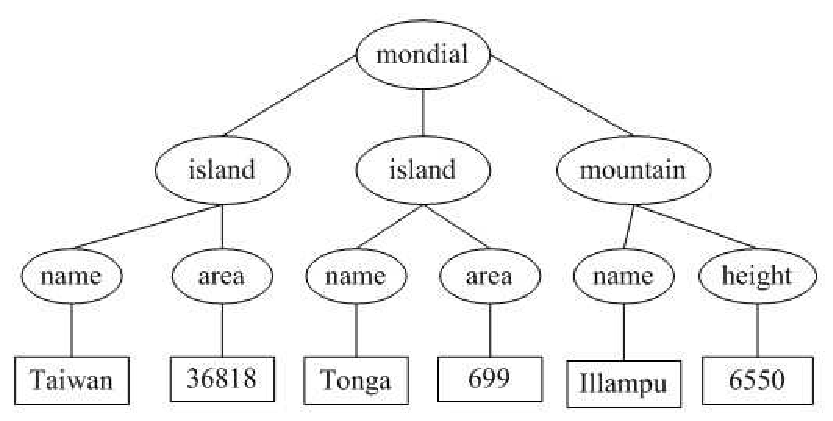
\includegraphics[width=0.4\textwidth]{XML}
\caption{树状结构}\label{fig:xml}
\vspace{\baselineskip}
\end{figure}


其插入图片的代码及其说明如下。
\vspace{1em}\noindent\hrule
\begin{verbatim}
\begin{figure}[htbp]
\centering
\includegraphics[width=0.4\textwidth]{文件名(.eps)}
\caption{标题}\label{标签名(通常为 fig:labelname)}
\vspace{\baselineskip} %表示图与正文空一行
\end{figure}
\end{verbatim}

\noindent\hrule

\begin{verbatim}
figure环境的可选参数[htbp]表示浮动图形所放置的位置,h (here)表示当前位置,t (top)表示页芯顶部,b (bottom)表示页芯底部,p (page)表示单独一页。在Word等软件中,图片通常插入到当前位置,如果当前页的剩余空间不够,图片将被移动到下一页,当前页就会出现很大的空白,其人工调整工作非常不便。由LaTeX提供的浮动图片功能,总是会按h->t->b->p的次序处理选项中的字母,自动调整图片的位置,大大减轻了工作量。
\centering命令将后续内容转换成每行皆居中的格式。
"\includegraphics"的可选参数用来设置图片插入文中的水平宽度,一般表示为正文宽度(\textwidth)的倍数。
\caption命令可选参数“标签名”为英文形式,一般不以图片或表格的数字顺序作为标签,而应包含一定的图片或表格信息,以便于文中引用(若图片、表格、公式、章节和参考文献等在文中出现的先后顺序发生了变化,其标注序号及其文中引用序号也会跟着发生变化,这一点是Word等软件所不能做到的)。另外,图题或表题并不会因为分页而与图片或表格体分置于两页,章节等各级标题也不会置于某页的最底部,LaTeX系统会自动调整它们在正文中的位置,这也是Word等软件所无法匹敌的。
\vspace将产生一定高度的竖直空白,必选参数为负值表示将后续文字位置向上提升,参数值可自行调整。em为长度单位,相当于大写字母M的宽度。\vspace{\baselineskip} 表示图与正文空一行。
引用方法:“见图~\ref{fig:figname}”、“如图~\ref{fig:figname}~所示”等。
\end{verbatim}

\noindent\hrule\vspace{1em}

若需要将~2~张及以上的图片并排插入到一行中,则需要采用\verb|minipage|环境,如图~\ref{fig:dd}~和图~\ref{fig:ds}~所示。
\begin{figure}[htbp]
\centering
\begin{minipage}{0.4\textwidth}
\centering
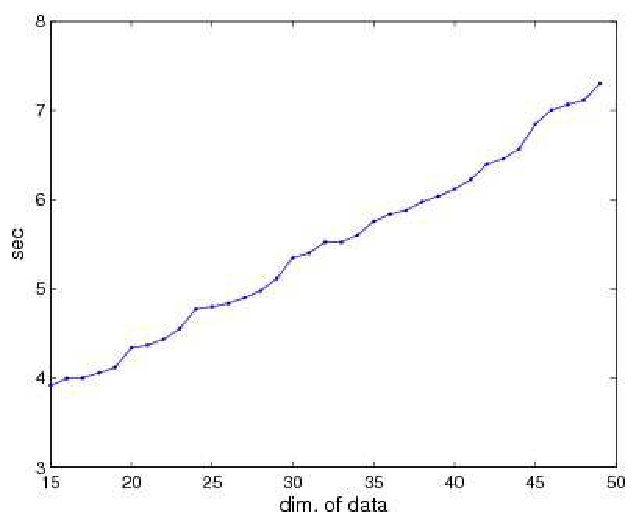
\includegraphics[width=\textwidth]{dataDimensions}
\caption{数据维数的变化}\label{fig:dd}
\end{minipage}
\begin{minipage}{0.4\textwidth}
\centering
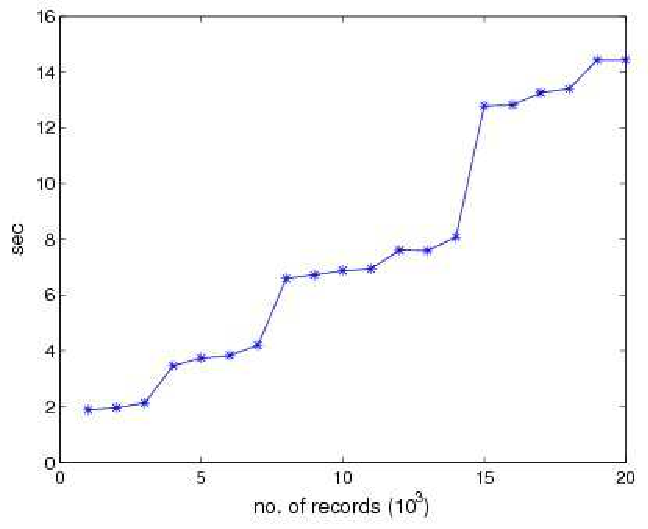
\includegraphics[width=\textwidth]{dataSize}
\caption{数据规模的变化}\label{fig:ds}
\end{minipage}
\vspace{\baselineskip}
\end{figure}

其代码如下所示。
\vspace{1em}\noindent\hrule
\begin{verbatim}
\begin{figure}[htbp]
\centering
\begin{minipage}{0.4\textwidth}
\centering
\includegraphics[width=\textwidth]{文件名}
\caption{标题}\label{fig:f1}
\end{minipage}
\begin{minipage}{0.4\textwidth}
\centering
\includegraphics[width=\textwidth]{文件名}
\caption{标题}\label{fig:f2}
\end{minipage}\vspace{\baselineskip}
\end{figure}
\end{verbatim}

\noindent\hrule

\begin{verbatim}
minipage环境的必选参数用来设置小页的宽度,若需要在一行中插入n个等宽图片,则每个小页的宽度应略小于(1/n)\textwidth。
\end{verbatim}

\noindent\hrule

\section{具有子图的图片插入方法}

图中若含有子图时,需要调用~subfigure~宏包, 如图~\ref{fig:subfig}~所示。
\begin{figure}[htbp]
  \centering
  \subfigure[Data Dimensions]{\label{fig:subfig:datadim}
                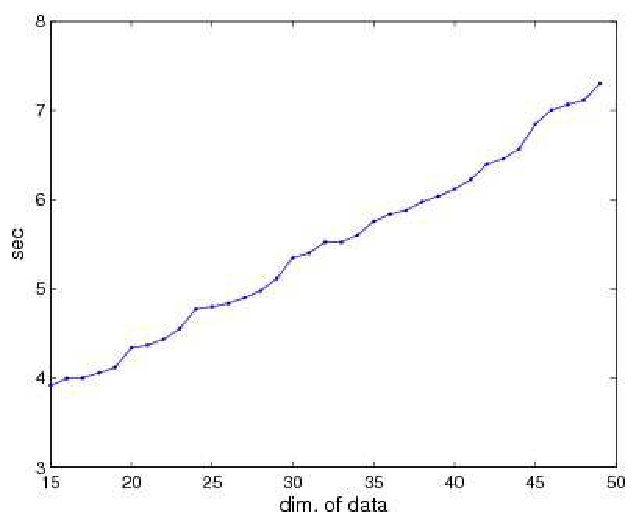
\includegraphics[width=0.4\textwidth]{dataDimensions}}
  \subfigure[Data Size]{\label{fig:subfig:datasize}
                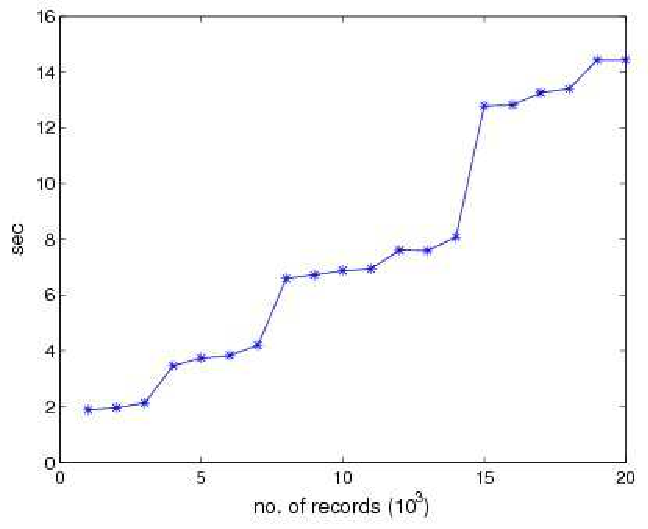
\includegraphics[width=0.4\textwidth]{dataSize}}
  \caption{Scalability of data}\label{fig:subfig}
\vspace{\baselineskip}
\end{figure}

其代码及其说明如下。
\vspace{1em}\noindent\hrule

\begin{verbatim}
\begin{figure}[htbp]
  \centering
  \subfigure[第1个子图标题]{
            \label{第1个子图标签(通常为 fig:subfig1:subsubfig1)}
            \includegraphics[width=0.4\textwidth]{文件名}}
  \subfigure[第2个子图标题]{
            \label{第2个子图标签(通常为 fig:subfig1:subsubfig2)}
            \includegraphics[width=0.4\textwidth]{文件名}}
  \caption{总标题}\label{总标签(通常为 fig:subfig1)}
\vspace{\baselineskip}
\end{figure}
\end{verbatim}

\noindent\hrule

\begin{verbatim}
子图的标签实际上可以随意设定,只要不重复就行。但为了更好的可读性,我们建议fig:subfig:subsubfig格式命名,这样我们从标签名就可以知道这是一个子图引用。
引用方法:总图的引用方法同本章第1节,子图的引用方法用\ref{fig:subfig:subsubfig}来代替。
\end{verbatim}

\noindent\hrule\vspace{1em}

子图的引用示例:如图~\ref{fig:subfig:datadim}~和图~\ref{fig:subfig:datasize}~所示。

若想获得插图方法的更多信息,参见网络上的~\href{ftp://ftp.tex.ac.uk/tex-archive/info/epslatex.pdf}{Using Imported Graphics in \LaTeX and pdf\LaTeX}~文档。 
%\clearpage{\pagestyle{empty}\cleardoublepage}
%% !Mode:: "TeX:UTF-8"

\chapter{表格的绘制方法}
\section{研究生毕业设计论文的绘表规范}

表应有自明性。表格不加左、右边线。表的编排建议采用国际通行的三线表。表内中文书写使用宋体五号字。

每个表格之上均应有表题(由表序和表名组成)。表序一般按章编排,如第~1~章第一个插表的序号为“表~1-1”等。表序与表名之间空两格,
表名使用中文五号字,居中。表名中不允许使用标点符号,表名后不加标点。
表头设计应简单明了,尽量不用斜线。表头中可采用化学,物理量等专业符号。

全表如用同一单位,则将单位符号移至表头右上角,加圆括号。
表中数据应准确无误,书写清楚。数字空缺的格内加横线“-”(占~2~个数字宽度)。表内文字或数字上、下或左、右相同时,
采用通栏处理方式,不允许用“〃”、“同上”之类的写法。

表内文字使用宋体五号字,垂直居中书写,起行空一格、转行顶格、句末不加标点。
如某个表需要转页接排,在随后的各页上应重复表的编号。编号后加“(续表)”,表题可省略。续表应重复表头。
表格绘制完成之后,与正文空一行。

\section{普通表格的绘制方法}

表格应具有三线表格式,因此需要调用~booktabs~宏包,其标准格式如表~\ref{tab:table1}~所示。
\begin{table}[htbp]
\caption{符合本科生毕业论文绘图规范的表格}\label{tab:table1}
\vspace{0.5em}\centering\wuhao
\begin{tabular}{ccccc}
\toprule[1.5pt]
$D$(in) & $P_u$(lbs) & $u_u$(in) & $\beta$ & $G_f$(psi.in)\\
\midrule[1pt]
 5 & 269.8 & 0.000674 & 1.79 & 0.04089\\
10 & 421.0 & 0.001035 & 3.59 & 0.04089\\
20 & 640.2 & 0.001565 & 7.18 & 0.04089\\
 5 & 269.8 & 0.000674 & 1.79 & 0.04089\\
10 & 421.0 & 0.001035 & 3.59 & 0.04089\\
20 & 640.2 & 0.001565 & 7.18 & 0.04089\\
 5 & 269.8 & 0.000674 & 1.79 & 0.04089\\
10 & 421.0 & 0.001035 & 3.59 & 0.04089\\
20 & 640.2 & 0.001565 & 7.18 & 0.04089\\
 5 & 269.8 & 0.000674 & 1.79 & 0.04089\\
10 & 421.0 & 0.001035 & 3.59 & 0.04089\\
20 & 640.2 & 0.001565 & 7.18 & 0.04089\\
\bottomrule[1.5pt]
\end{tabular}
\vspace{\baselineskip}
\end{table}

其绘制表格的代码及其说明如下。
\vspace{1em}\noindent\hrule

\begin{verbatim}
\begin{table}[htbp]
\caption{表标题}\label{标签名(通常为 tab:tablename)}
\vspace{0.5em}\centering\wuhao
\begin{tabular}{cc...c}
\toprule[1.5pt]
表头第1个格   & 表头第2个格   & ... & 表头第n个格  \\
\midrule[1pt]
表中数据(1,1) & 表中数据(1,2) & ... & 表中数据(1,n)\\
表中数据(2,1) & 表中数据(2,2) & ... & 表中数据(2,n)\\
表中数据(3,1) & 表中数据(3,2) & ... & 表中数据(3,n)\\
表中数据(4,1) & 表中数据(4,2) & ... & 表中数据(4,n)\\
...................................................\\
表中数据(m,1) & 表中数据(m,2) & ... & 表中数据(m,n)\\
\bottomrule[1.5pt]
\end{tabular}
\vspace{\baselineskip}
\end{table}
\end{verbatim}

\noindent\hrule

\begin{verbatim}
table环境是一个将表格嵌入文本的浮动环境。
\wuhao命令将表格的字号设置为五号字(10.5pt),在绘制表格结束退出时,不需要将字号再改回为\xiaosi,正文字号默认为小四号字(12pt)。
tabular环境的必选参数由每列对应一个格式字符所组成:c表示居中,l表示左对齐,r表示右对齐,其总个数应与表的列数相同。此外,@{文本}可以出现在任意两个上述的列格式之间,其中的文本将被插入每一行的同一位置。表格的各行以\\分隔,同一行的各列则以&分隔。
\toprule、\midrule和\bottomrule三个命令是由booktabs宏包提供的,其中\toprule和\bottomrule分别用来绘制表格的第一条(表格最顶部)和第三条(表格最底部)水平线,\midrule用来绘制第二条(表头之下)水平线,且第一条和第三条水平线的线宽为1.5pt,第二条水平线的线宽为1pt。
引用方法:“如表~\ref{tab:tablename}~所示”。
\end{verbatim}

\noindent\hrule

\section{长表格的绘制方法}

长表格是当表格在当前页排不下而需要转页接排的情况下所采用的一种表格环境。若长表格仍按照普通表格的绘制方法来获得,
其所使用的\verb|table|浮动环境无法实现表格的换页接排功能,表格下方过长部分会排在表格第1页的页脚以下。为了能够实现长表格的转页接排功能,
需要调用~longtable~宏包,由于长表格是跨页的文本内容,因此只需要单独的\verb|longtable|环境,所绘制的长表格的格式如表~\ref{tab:table2}~所示。

此长表格~\ref{tab:table2}~第~2~页的标题“编号(续表)”和表头是通过代码自动添加上去的,无需人工添加,若表格在页面中的竖直位置发生了变化,长表格在第~2~页
及之后各页的标题和表头位置能够始终处于各页的最顶部,也无需人工调整,\LaTeX~系统的这一优点是~Word~等软件所无法企及的。

下段内容是为了让下面的长表格分居两页,看到表标题“编号(续表)”的效果。摘录于《你若安好,便是晴天 -- 林徽因传》片段:

她叫林徽因,出生于杭州,是许多人梦中期待的白莲。她在雨雾之都伦敦,发生过一场空前绝后的康桥之恋。她爱过三个男子,爱得清醒,也爱得平静。徐志摩为她徜徉在康桥,深情地等待一场旧梦可以归来。梁思成与她携手走过千山万水,为完成使命而相约白头。金岳霖为她终身不娶,痴心不改地守候一世。可她懂得人生飘忽不定,要学会随遇而安。
真正的平静,不是避开车马喧嚣,而是在心中修篱种菊。尽管如流往事,每一天都涛声依旧,只要我们消除执念,便可寂静安然。愿每个人在纷呈世相中不会迷失荒径,可以端坐磐石上,醉倒落花前。
如果可以,请让我预支一段如莲的时光,哪怕将来某一天加倍偿还。这个雨季会在何时停歇,无从知晓。但我知道,你若安好,便是晴天。					
\wuhao\begin{longtable}{ccc}
\caption{天津大学各学院名称一览}\label{tab:table2}
 \vspace{0.5em}\\
\toprule[1.5pt] 学院名称 & 网址 & 联系电话  \\ \midrule[1pt]
\endfirsthead
\multicolumn{3}{c}{表~\thetable(续表)}\vspace{0.5em}\\
\toprule[1.5pt] 学院名称 & 网址 & 联系电话  \\ \midrule[1pt]
\endhead
\bottomrule[1.5pt]
\endfoot
机械工程学院& \url{http://tdjxxy.tju.edu.cn/}& 87401979\\
精密仪器与光电子工程学院&  \url{http://www2.tju.edu.cn/colleges/precision/cn/}& 27404775\\
电子信息工程学院& \url{http://www.tju.edu.cn/seie}& 27406956\\
电气与自动化工程学院& \url{http://www2.tju.edu.cn/colleges/automate/}& 27405477\\
建筑工程学院& \url{http://www2.tju.edu.cn/colleges/civil/}& 27404072\\
化工学院& \url{http://chemeng.tju.edu.cn/}& 27403389\\
材料科学与工程学院& \url{http://mse.tju.edu.cn}& 27406693 \\
建筑学院& \url{http://hgw022072.chinaw3.com/}& 27402724-2111\\
求是学部\\
管理与经济学部&	\url{ http://sm.tju.edu.cn}& 27403423\\
理学院& \url{ http://www.tju.edu.cn/science/}& 27404118\\
文法学院& \url{ http://www2.tju.edu.cn/colleges/sociology/new/}& 27403691\\
软件学院& \url{http://scs.tju.edu.cn}& 87401540\\
计算机科学与技术学院& \url{http://cs.tju.edu.cn/}& 27406538\\
马克思主义学院& \url{http://www2.tju.edu.cn/colleges/marxism/}& 27405348\\
环境科学与工程学院& \url{http://www.tju.edu.cn/see}& 87402072\\
药物科学与技术学院& \url{http://www2.tju.edu.cn/colleges/pharmtier/}& 87401830\\
教育学院& \url{http://soe.tju.edu.cn/}& 27401028\\
职业技术教育学院& \url{http://202.113.0.248:8888}\\
继续教育学院& \url{http://aectu.tju.edu.cn/}& 27406298\\
仁爱学院& \url{http://www.tjrac.edu.cn/}& 68579990\\
农业与生物工程学院& \url{http://202.113.13.169/site/nongxueyuan/}& 87402171\\
国际教育学院 & \url{http://www.ietju.com/}& 27406147\\
网络教育学院 & \url{http://www.etju.com/}& 27426952 \\

\end{longtable}\xiaosi
\vspace{\baselineskip}

绘制长表格的代码及其说明如下。
\vspace{1em}\noindent\hrule

\begin{verbatim}
\wuhao\begin{longtable}{cc...c}
\caption{表标题}\label{标签名(通常为 tab:tablename)}\\
\toprule[1.5pt] 表头第1个格 & 表头第2个格 & ... & 表头第n个格\\ \midrule[1pt]
\endfirsthead
\multicolumn{n}{c}{表~\thetable(续表)}\vspace{0.5em}\\
\toprule[1.5pt] 表头第1个格 & 表头第2个格 & ... & 表头第n个格\\ \midrule[1pt]
\endhead
\bottomrule[1.5pt]
\endfoot
表中数据(1,1) & 表中数据(1,2) & ... & 表中数据(1,n)\\
表中数据(2,1) & 表中数据(2,2) & ... & 表中数据(2,n)\\
...................................................\\
表中数据(m,1) & 表中数据(m,2) & ... & 表中数据(m,n)\\
\end{longtable}\xiaosi
\end{verbatim}

\noindent\hrule
\begin{verbatim}
在绘制长表格的前面留出一个空白行,并在第2行的一开始全局定义长表格的字号为五号字,这样能够保证长表格之前段落的行距保持不变。
在绘制长表格结束后,需要\xiaosi命令重新将字号改为小四号字。
\endhead之前的文字描述的是第2页及其之后各页的标题或表头;
\endfirsthead之前的文字描述的是第1页的标题和表头,若无此命令,则第1页的表头和标题由\endhead命令确定;
同理,\endfoot之前的文字描述的是除最后一页之外每页的表格底部内容;
\endlastfoot之前的文字描述的是最后一页的表格底部内容,若无此命令,
则最后一页的表格底部内容由\endfoot命令确定;由于规范中长表格每页底部内容均相同(水平粗线),因此模板中没有用到\endlastfoot命令。
\end{verbatim}

\noindent\hrule
\section{列宽可调表格的绘制方法}
论文中能用到列宽可调表格的情况共有两种:一种是当插入的表格某一单元格内容过长以至于一行放不下的情况,
另一种是当对公式中首次出现的物理量符号进行注释的情况。这两种情况都需要调用~tabularx~宏包。下面将分别对这两种情况下可调表格的绘制方法进行阐述。
\subsection{表格内某单元格内容过长的情况}

首先给出这种情况下的一个例子如表~\ref{tab:table3}~所示。
\begin{table}[htbp]
\caption{最小的三个正整数的英文表示法}\label{tab:table3}
\vspace{0.5em}\wuhao
\begin{tabularx}{\textwidth}{llX}
\toprule[1.5pt]
Value & Name & Alternate names, and names for sets of the given size\\\midrule[1pt]
1 & One & ace, single, singleton, unary, unit, unity\\
2 & Two & binary, brace, couple, couplet, distich, deuce, double, doubleton, duad, duality, duet, duo, dyad, pair, snake eyes, span, twain, twosome, yoke\\
3 & Three & deuce-ace, leash, set, tercet, ternary, ternion, terzetto, threesome, tierce, trey, triad, trine, trinity, trio, triplet, troika, hat-trick\\\bottomrule[1.5pt]
\end{tabularx}
\vspace{\baselineskip}
\end{table}
绘制这种表格的代码及其说明如下。
\vspace{1em}\noindent\hrule
\begin{verbatim}
\begin{table}[htbp]
\caption{表标题}\label{标签名(通常为 tab:tablename)}
\vspace{0.5em}\wuhao
\begin{tabularx}{\textwidth}{l...X...l}
\toprule[1.5pt]
表头第1个格   & ... & 表头第X个格   & ... & 表头第n个格  \\
\midrule[1pt]
表中数据(1,1) & ... & 表中数据(1,X) & ... & 表中数据(1,n)\\
表中数据(2,1) & ... & 表中数据(2,X) & ... & 表中数据(2,n)\\
.........................................................\\
表中数据(m,1) & ... & 表中数据(m,X) & ... & 表中数据(m,n)\\
\bottomrule[1.5pt]
\end{tabularx}
\vspace{\baselineskip}
\end{table}
\end{verbatim}

\noindent\hrule
\begin{verbatim}
tabularx环境共有两个必选参数:第1个参数用来确定表格的总宽度,这里取为排版表格能达到的最大宽度——正文宽度\textwidth;第2个参数用来确定每列格式,其中标为X的项表示该列的宽度可调,其宽度值由表格总宽度确定。
标为X的列一般选为单元格内容过长而无法置于一行的列,这样使得该列内容能够根据表格总宽度自动分行。若列格式中存在不止一个X项,则这些标为X的列的列宽相同,因此,一般不将内容较短的列设为X。
标为X的列均为左对齐,因此其余列一般选为l(左对齐),这样可使得表格美观,但也可以选为c或r。
\end{verbatim}

\noindent\hrule
\subsection{对物理量符号进行注释的情况}
为使得对公式中物理量符号注释的转行与破折号“———”后第一个字对齐,此处最好采用表格环境。此表格无任何线条,左对齐,
且在破折号处对齐,一共有“式中”二字、物理量符号和注释三列,表格的总宽度可选为文本宽度,因此应该采用\verb|tabularx|环境。
由\verb|tabularx|环境生成的对公式中物理量符号进行注释的公式如式(\ref{eq:1})所示。
%\vspace*{10pt}

\begin{equation}\label{eq:1}
\ddot{\boldsymbol{\rho}}-\frac{\mu}{R_{t}^{3}}\left(3\mathbf{R_{t}}\frac{\mathbf{R_{t}\rho}}{R_{t}^{2}}-\boldsymbol{\rho}\right)=\mathbf{a}
\end{equation}

\begin{tabularx}{\textwidth}{@{}l@{\quad}r@{———}X@{}}
式中& $\bm{\rho}$ &追踪飞行器与目标飞行器之间的相对位置矢量;\\
&  $\bm{\ddot{\rho}}$&追踪飞行器与目标飞行器之间的相对加速度;\\
&  $\mathbf{a}$   &推力所产生的加速度;\\
&  $\mathbf{R_t}$ & 目标飞行器在惯性坐标系中的位置矢量;\\
&  $\omega_{t}$ & 目标飞行器的轨道角速度;\\
&  $\mathbf{g}$ & 重力加速度,$=\frac{\mu}{R_{t}^{3}}\left(
3\mathbf{R_{t}}\frac{\mathbf{R_{t}\rho}}{R_{t}^{2}}-\bm{\rho}\right)=\omega_{t}^{2}\frac{R_{t}}{p}\left(
3\mathbf{R_{t}}\frac{\mathbf{R_{t}\rho}}{R_{t}^{2}}-\bm{\rho}\right)$,这里~$p$~是目标飞行器的轨道半通径。
\end{tabularx}
\vspace{\wordsep}

其中生成注释部分的代码及其说明如下。

\vspace{1em}\noindent\hrule

\begin{verbatim}
\begin{tabularx}{\textwidth}{@{}l@{\quad}r@{— — —}X@{}}
式中 & symbol-1 & symbol-1的注释内容;\\
     & symbol-2 & symbol-2的注释内容;\\
     .............................;\\
     & symbol-m & symbol-m的注释内容。
\end{tabularx}\vspace{\wordsep}
\end{verbatim}

\noindent\hrule

\begin{verbatim}
tabularx环境的第1个参数选为正文宽度,第2个参数里面各个符号的意义为:
    第1个@{}表示在“式中”二字左侧不插入任何文本,“式中”二字能够在正文中左对齐,若无此项,则“式中”二字左侧会留出一定的空白;
    @{\quad}表示在“式中”和物理量符号间插入一个空铅宽度的空白;
    @{— — —}实现插入破折号的功能,它由三个1/2的中文破折号构成;
    第2个@{}表示在注释内容靠近正文右边界的地方能够实现右对齐。
\end{verbatim}

\noindent\hrule\vspace{1em}

由此方法生成的注释内容应紧邻待注释公式并置于其下方,因此不能将代码放入\verb|table|浮动环境中。但此方法不能实现自动转页接排,
可能会在当前页剩余空间不够时,全部移动到下一页而导致当前页出现很大空白。因此在需要转页处理时,还请您手动将需要转页的代码放入一个
新的\verb|tabularx|环境中,将原来的一个\verb|tabularx|环境拆分为两个\verb|tabularx|环境。

若想获得绘制表格的更多信息,参见网络上的~\href{http://www.tug.org/pracjourn/2007-1/mori/}{Tables in \LaTeXe: Packages and Methods}~文档。


%\clearpage{\pagestyle{empty}\cleardoublepage}
%% !Mode:: "TeX:UTF-8"

\chapter{数学公式的输入方法}
\section{研究生毕业设计论文的公式规范}

论文中的公式应另起行,原则上应居中书写,与周围文字留有足够的空间区分开。
若公式前有文字(如“解”、“假定”等),文字空两格写,公式仍居中写。公式末不加标点。

公式应标注序号,并将序号置于括号内。 公式序号按章编排,如第~1~章第一个公式序号为“(1-1)”。公式的序号右端对齐。

公式较长时最好在等号“=”处转行,如难实现,则可在~$+$、$-$、$\times$、$\div$~运算符号处转行,转行时运算符号仅书写于转行式前,不重复书写。

文中引用公式时,一般用“见式~(1-1)”或“由公式~(1-1)”。

公式中用斜线表示“除”的关系时应采用括号,以免含糊不清,如~$a/(b\cos x)$。通常“乘”的关系在前,如~$a\cos x/b$而不写成~$(a/b)\cos x$。

不能用文字形式表示等式,如:$\textnormal{刚度}=\frac{{\textnormal{受力}}}{{\textnormal{受力方向的位移}}}$。

对于数学公式的输入方法,网络上有一个比较全面权威的文档\textbf{~\href{http://tug.ctan.org/cgi-bin/ctanPackageInformation.py?id=voss-mathmode}{Math mode}}~请大家事先大概浏览一下。下面将对学位论文中主要用到的数学公式排版形式进行阐述。

\section{生成~\LaTeX~数学公式的两种方法}
对于先前没有接触过~\LaTeX~的人来说,编写~\LaTeX~数学公式是一件很繁琐的事,尤其是对复杂的数学公式来说,更可以说是一件难以完成的任务。
实际上,生成~\LaTeX~数学公式有两种较为简便的方法,一种是基于~MathType~数学公式编辑器的方法,另一种是基于~MATLAB~商业数学软件的方法,
下面将分别对这两种数学公式的生成方法作一下简单介绍。

\subsection{基于~MathType~软件的数学公式生成方法}
MathType~是一款功能强大的数学公式编辑器软件,能够用来在文本环境中插入~Windows OLE~图形格式的复杂数学公式,所以应用比较普遍。但此软件只有~30~天的试用期,之后若再继续使用则需要付费购买才行。网络上有很多破解版的~MathType~软件可供下载免费使用,
笔者推荐下载安装版本号在~6.5~之上的中文破解版。

在安装好~MathType~之后,若在输入窗口中编写数学公式,复制到剪贴板上的仍然是图形格式的对象。
若希望得到可插入到~\LaTeX~编辑器中的文本格式对象,则需要对~MathType~软件做一下简单的设置:在~MathType~最上排的按钮中依次选择“参数选项
$\to$转换”,在弹出的对话窗中选中“转换到其它语言(文字):”,在转换下拉框中选择“Tex~--~--~LaTeX 2.09 and later”,并将对话框最下方的两个复选框全部勾掉,点击确定,这样,再从输入窗口中复制出来的对象就是文本格式的了,就可以直接将其粘贴到~\LaTeX~
编辑器中了。按照这种方法生成的数学公式两端分别有标记\verb|\[|和标记\verb|\]|,在这两个标记之间才是真正的数学公式代码。

若希望从~MathType~输入窗口中复制出来的对象为图形格式,则只需再选中“公示对象(Windows OLE~图形)”即可。

\subsection{基于~MATLAB~软件的数学公式生成方法}

MATLAB~是矩阵实验室(Matrix Laboratory)的简称,是美国~MathWorks~公司出品的商业数学软件。它是当今科研领域最常用的应用软件之一,
具有强大的矩阵计算、符号运算和数据可视化功能,是一种简单易用、可扩展的系统开发环境和平台。

MATLAB~中提供了一个~latex~函数,它可将符号表达式转化为~\LaTeX~数学公式的形式。其语法形式为~latex(s),其中,~s~为符号表达式,
之后再将~latex~函数的运算结果直接粘贴到~\LaTeX~编辑器中。从~\LaTeX~数学公式中可以发现,其中可能包含如下符号组合:

\begin{verbatim*}
\qquad=两个空铅(quad)宽度
\quad=一个空铅宽度
\;=5/18空铅宽度
\:=4/18空铅宽度
\,=3/18空铅宽度
\!=-3/18空铅宽度
\ =一个空格
\end{verbatim*}

所以最好将上述符号组合从数学公式中删除,从而使数学公式显得匀称美观。

对于~Word~等软件的使用者来说,在我们通过~MATLAB~运算得到符号表达式形式的运算结果时,在~Word~中插入运算结果需要借助于~MathType~软件,
通过在~MathType~中输入和~MATLAB~运算结果相对应的数学表达形式,之后再将~MathType~数学表达式转换为图形格式粘贴到~Word~中。实际上,
也可以将~MATLAB~中采用~latex~函数运行的结果直接粘贴到~MathType~中,再继续上述步骤,这样可以大大节省输入公式所需要的时间。
此方法在~MathType~6.5c~上验证通过,若您粘入到~MathType~中的仍然为从~MATLAB~中导入的代码,请您更新~MathType~软件。

\section{数学字体}
在数学模式下,常用的数学字体命令有如下几种:

\begin{verbatim}
\mathnormal或无命令 用数学字体打印文本;
\mathit             用斜体(\itshape)打印文本;
\mathbf             用粗体(\bfseries)打印文本;
\mathrm             用罗马体(\rmfamily)打印文本;
\mathsf             用无衬线字体(\sffamily)打印文本;
\mathtt             用打印机字体(\ttfamily)打印文本;
\mathcal            用书写体打印文本;
\end{verbatim}

在学位论文撰写中,只需要用到上面提到的~\verb|\mathit|、\verb|\mathbf|~和~\verb|\mathrm|~命令。若要得到~Times New Roman~的数学字体,则需要调用~txfonts~宏包(此宏包实际上采用的是~Nimbus Roman No9 L~字体,
它是开源系统中使用的免费字体,其字符字体与~Times New Roman~字体几乎完全相同);若要得到粗体数学字体,则需要调用~bm~宏包。表~\ref{tab:fonts}~中分别列出了得到阿拉伯数字、拉丁字母和希腊字母
各种数学字体的命令。

\begin{table}[htbp]
\caption{常用数学字体命令一览}\label{tab:fonts}
\vspace{0.5em}\centering\wuhao
\begin{tabular}{llll}
\toprule
 & 阿拉伯数字\&大写希腊字母 & 大小写拉丁字母 & 小写希腊字母  \\
\midrule
斜体 & \verb|\mathit{}| & \verb|无命令| & \verb|无命令|\\
粗斜体 & \verb|\bm{\mathit{}}| & \verb|\bm{}| & \verb|\bm{}|\\
直立体 & \verb|无命令| & \verb|\mathrm{}| & \verb|字母后加up|\\
粗体 & \verb|\mathbf{}或\bm{}| & \verb|\mathbf{}| & \verb|\bm{字母后加up}|\\
\bottomrule
\end{tabular}
\vspace{\baselineskip}
\end{table}

\noindent 下面列出了一些应采用直立数学字体的数学常数和数学符号。

\vspace{-0.5em}\begin{center}\begin{tabularx}{0.7\textwidth}{XX}
$\mathrm{d}$、 $\mathrm{D}$、 $\mathrm{p}$~———微分算子 & $\mathrm{e}$~———自然对数之底数\\
$\mathrm{i}$、 $\mathrm{j}$~———虚数单位 & $\piup$———圆周率\\
\end{tabularx}\end{center}

\section{行内公式}
出现在正文一行之内的公式称为行内公式,例如~$f(x)=\int_{a}^{b}\frac{\sin{x}}{x}\mathrm{d}x$。对于非矩阵和非多行形式的行内公式,一般不会使得行距发生变化,而~Word~等软件却会根据行内公式的竖直距离而自动调节行距,如图~\ref{fig:hangju}~所示。

\begin{figure}[htbp]
\centering
\subfigure[由~\LaTeX~系统生成的行内公式]{\label{fig:subfig:latex}
                \fbox{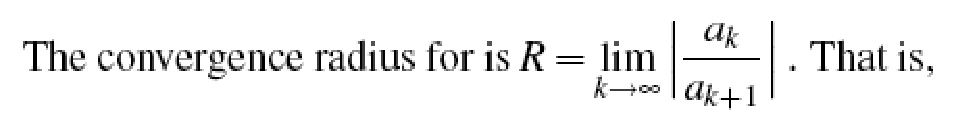
\includegraphics[width=0.55\textwidth]{latex}}}
\subfigure[由~Word软件生成的~.doc~格式行内公式]{\label{fig:subfig:word}
                \fbox{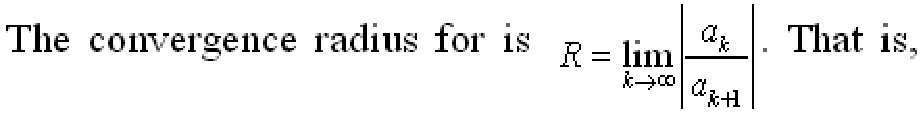
\includegraphics[width=0.55\textwidth]{word}}}
\subfigure[由~Word软件生成的~.pdf~格式行内公式]{\label{fig:subfig:pdf}
                \fbox{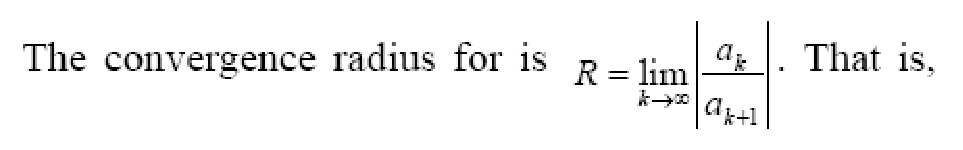
\includegraphics[width=0.55\textwidth]{pdf}}}

\caption{由~\LaTeX~和~Word~生成的~3~种行内公式屏显效果}\label{fig:hangju}
\vspace{-1em}
\end{figure}

这三幅图分别为~\LaTeX~和~Word~生成的行内公式屏显效果,从图中可看出,在~\LaTeX~文本含有公式的行内,在正文与公式之间对接工整,行距不变;而在~Word~文本含有公式的行内,在正文与公式之间对接不齐,行距变大。因此从这一点来说,
\LaTeX~系统在数学公式的排版上具有很大优势。

\LaTeX~提供的行内公式最简单、最有效的方法是采用~\TeX~本来的标记———开始和结束标记都写作~\$,例如本段开始的例子可由下面的输入得到。
\verb|$f(x)=\int_{a}^{b}\frac{\sin{x}}{x}\mathrm{d}x$|

\section{行间公式}
位于两行之间的公式称为行间公式,每个公式都是一个单独的段落,例如
\[\int_a^b{f\left(x\right)\mathrm{d}x}=\lim_{\left\|\Delta{x_i}\right\|\to 0}\sum_i{f\left(\xi_i\right)\Delta{x_i}}\]
除人工编号外,\LaTeX~各种类型行间公式的标记见表~\ref{tab:eqtag}。
\begin{table}[htbp]
\caption{各种类型行间公式的标记}\label{tab:eqtag}
\vspace{0.5em}\centering\wuhao
\begin{tabularx}{\textwidth}{cll}
\toprule
& 无编号 & 自动编号\\
\midrule
单行公式& \verb|\begin{displaymath}... \end{displaymath}|& \verb|\begin{equation}... \end{equation}|\\
        & 或~\verb|\[...\]| & \\
多行公式& \verb|\begin{eqnarray*}... \end{eqnarray*}|& \verb|\begin{eqnarray}... \end{eqnarray}|\\
\bottomrule
\end{tabularx}
\end{table}

另外,在自动编号的某行公式行尾添加标签~\verb|\nonumber|,可将该行转换为无编号形式。

行间多行公式需采用~\verb|eqnarray|~或~\verb|eqnarray*|~环境,它默认是一个列格式为~\verb|rcl|~的~3~列矩阵,并且中间列的字号要小一些,因此通常只将需要对齐的运算符号(通常为等号“=”)置于中间列。

\section{可自动调整大小的定界符}
若在左右两个定界符之前分别添加命令~\verb|\left|~和~\verb|\right|,则定界符可根据所包围公式大小自动调整其尺寸,这可从式(\ref{nodelimiter})和式(\ref{delimiter})中看出。
\begin{equation}\label{nodelimiter}
(\sum_{k=\frac12}^{N^2})
\end{equation}
\begin{equation}\label{delimiter}
\left(\sum_{k=\frac12}^{N^2}\right)
\end{equation}
式(\ref{nodelimiter})和式(\ref{delimiter})是在~\LaTeX~中分别输入如下代码得到的。
\begin{verbatim}
(\sum_{k=\frac12}^{N^2})
\left(\sum_{k=\frac12}^{N^2}\right)
\end{verbatim}
\verb|\left|~和~\verb|\right|~总是成对出现的,若只需在公式一侧有可自动调整大小的定界符,则只要用“.”代替另一侧那个无需打印出来的定界符即可。

若想获得关于此部分内容的更多信息,可参见~\href{http://tug.ctan.org/cgi-bin/ctanPackageInformation.py?id=voss-mathmode}{Math mode}~文档的第~8~章“Brackets, braces and parentheses”。

\section{数学重音符号}
数学重音符号通常用来区分同一字母表示的不同变量,输入方法如下(需要调用~\verb|amsmath|~宏包):

\vspace{0.5em}\noindent\wuhao\begin{tabularx}{\textwidth}{Xc|Xc|Xc}
 \verb|\acute| & $\acute{a}$ & \verb|\mathring| & $\mathring{a}$ & \verb|\underbrace| & $\underbrace{a}$ \\
 \verb|\bar| & $\bar{a}$ & \verb|\overbrace| & $\overbrace{a}$ & \verb|\underleftarrow| & $\underleftarrow{a}$ \\
 \verb|\breve| & $\breve{a}$ & \verb|\overleftarrow| & $\overleftarrow{a}$ & \verb|\underleftrightarrow| & $\underleftrightarrow{a}$ \\
 \verb|\check| & $\check{a}$ & \verb|\overleftrightarrow| & $\overleftrightarrow{a}$ & \verb|\underline| & $\underline{a}$ \\
 \verb|\dddot| & $\dddot{a}$ & \verb|\overline| & $\overline{a}$ & \verb|\underrightarrow| & $\underrightarrow{a}$ \\
 \verb|\ddot| & $\ddot{a}$ & \verb|\overrightarrow| & $\overrightarrow{a}$ & \verb|\vec| & $\vec{a}$ \\
 \verb|\dot| & $\dot{a}$ & \verb|\tilde| & $\tilde{a}$ & \verb|\widehat| & $\widehat{a}$ \\
 \verb|\grave| & $\grave{a}$ & \verb|\underbar| & $\underbar{a}$ & \verb|\widetilde| & $\widetilde{a}$ \\
 \verb|\hat| & $\hat{a}$
\end{tabularx}\vspace{0.5em}
\xiaosi 当需要在字母~$i$~和~$j$~的上方添加重音符号时,为了去掉这两个字母顶上的小点,这两个字母应该分别改用~\verb|\imath|~和~\verb|\jmath|。

如果遇到某些符号不知道该采用什么命令能输出它时,则可通过~\href{http://detexify.kirelabs.org/classify.html}{Detexify$^2$~网站}来获取符号命令。若用鼠标左键在此网页的方框区域内画出你所要找的符号形状,则会在网页右方列出和你所画符号形状相近的~5~个符号及其相对应的~\LaTeX~输入命令。若所列出的符号中不包括你所要找的符号,还可通过点击“Select from the complete list!”的链接以得分从低到高的顺序列出所有符号及其相对应的~\LaTeX~输入命令。

最后,建议大家还以~\href{http://tug.ctan.org/cgi-bin/ctanPackageInformation.py?id=voss-mathmode}{Math mode}~这篇~pdf~文档作为主要参考。若要获得最为标准、美观的数学公式排版形式,可以查查文档中是否有和你所要的排版形式相同或相近的代码段,通过修改代码段以获得你所要的数学公式排版形式。


%\clearpage{\pagestyle{empty}\cleardoublepage}
%% !Mode:: "TeX:UTF-8"

\chapter{罗列和定理环境使用方法}

\section{单层罗列环境}
天津大学学位论文一般可采用两种罗列环境:一种是并列条目有同样标签的~\verb|itemize|~罗列环境,另一种是具有自动排序编号符号的~\verb|enumerate|~罗列环境。这两种罗列环境的样式参数可参考图~\ref{fig:list}。
\begin{figure}[htbp]
\centering
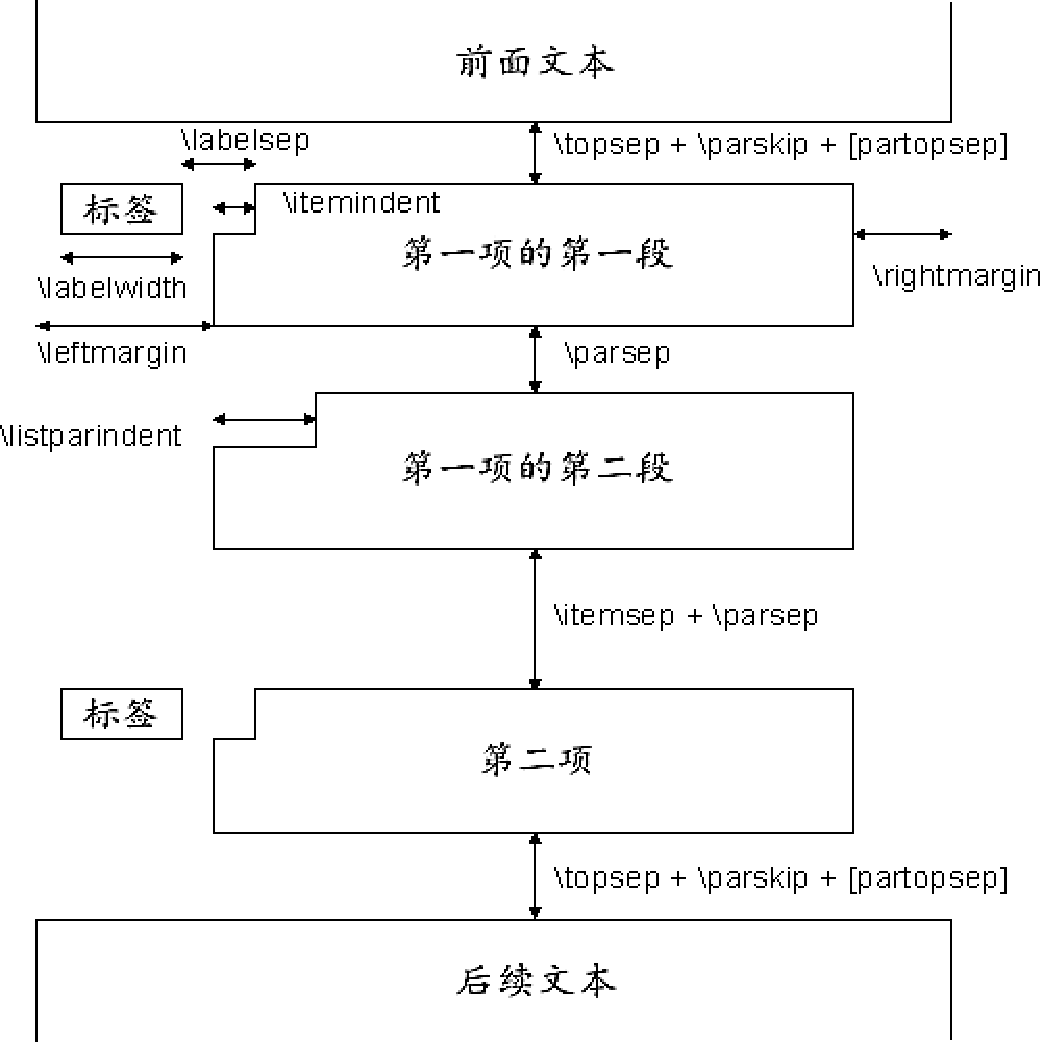
\includegraphics[width = 0.6\textwidth]{list}
\caption{罗列环境参数示意图}\label{fig:list}\vspace{-1em}
\end{figure}

通过调用~enumitem~宏包可以很方便地控制罗列环境的布局,其~format.tex~文件中的~\verb|\setitemize|~和~\verb|\setenumerate|~命令分别用来设置~\verb|itemize|~和~\verb|enumerate|~环境的样式参数。采用~\verb|itemize|~单层罗列环境的排版形式如下:

\begin{itemize}
\item 第一个条目文本内容
\item 第二个条目文本内容
\item 第三个条目文本内容
\end{itemize}

其代码如下

\begin{verbatim}
\begin{itemize}
  \item 第一个条目文本内容
  \item 第二个条目文本内容
  ...
  \item 第三个条目文本内容
\end{itemize}
\end{verbatim}

采用~\verb|enumerate|~单层罗列环境的排版形式如下:

\begin{enumerate}
\item 第一个条目文本内容
\item 第二个条目文本内容
\item 第三个条目文本内容
\end{enumerate}

其代码如下

\begin{verbatim}
\begin{enumerate}
  \item 第一个条目文本内容
  \item 第二个条目文本内容
  ...
  \item 第三个条目文本内容
\end{enumerate}
\end{verbatim}



\section{定理环境}

\begin{definition}[谱半径]\label{def:def1}
  称~$n$~阶方阵~$\mathbf{A}$~的全体特征值~$\lambda_1,\cdots,\lambda_n$~组成的集合为~$\mathbf{A}$~的谱,称
  $$\rho(\mathbf{A})=\max{\{|\lambda_1|,\cdots,|\lambda_n|\}}$$
\end{definition}
\begin{theorem}[相似充要条件]\label{lemma:l1}
  方阵$A$和$B$相似的充要条件是:~$A$~和~$B$~有全同的不变因子。
\end{theorem}
\begin{corollary}[推论1]\label{cor:cor1}
在赋范空间~$(X,\|\cdot\|)$~上定义~$d(x,y)=\|x-y\|$, 对任意~$x,y\in X$,~则~$(X,d)$~是距离空间。
\end{corollary}
\begin{proof}
  只需证明~$d(x,y)$~是距离。
\end{proof}
\newpage

定义代码如下:
\begin{verbatim}
 \begin{definition}[谱半径]\label{def:def1}
  称~$n$~阶方阵~$\mathbf{A}$~的全体特征值
  $\lambda_1,\cdots,\lambda_n$组成的集合为~$\mathbf{A}$~的谱,称
  $$\rho(\mathbf{A})=\max{\{|\lambda_1|,\cdots,|\lambda_n|\}}$$
\end{definition}
\end{verbatim}
\noindent\hrule

\vspace{0.1em}\noindent\hrule
\vspace{1em}
定理代码如下:
\begin{verbatim}
\begin{theorem}[相似充要条件]\label{lemma:l1}
  方阵$A$和$B$相似的充要条件是:$A$和$B$有全同的不变因子。
\end{theorem}
\end{verbatim}
\noindent\hrule\vspace{0.1em}

\noindent\hrule
\vspace{1em}
推论和证明代码如下:
\begin{verbatim}
\begin{corollary}[推论1]\label{cor:cor1}
在赋范空间~$(X,\|\cdot\|)$~上定义$d(x,y)=\|x-y\|$,
对任意$x,y\in X$,则$(X,d)$是距离空间。
\end{corollary}
\begin{proof}
  只需证明$d(x,y)$是距离。
\end{proof}
\end{verbatim}
\noindent\hrule\vspace{1em}

定理定义[]中是可选参数,用来说明定理的名称。其他环境格式书写与上面定理、定义、推论格式相同,可自己调用其他环境。
若需要书写定理定义等内容,而且带有顺序编号,需要采用如下环境。除了~\verb|proof|~环境之外,其余~9~个环境都可以有一个可选参数作为附加标题。

\begin{center}
\vspace{0.5em}\noindent\wuhao\begin{tabularx}{0.7\textwidth}{lX|lX}
定理 & \verb|theorem|~环境 & 定义 & \verb|definition|~环境 \\
例 & \verb|example|~环境 & 算法 & \verb|algorithm|~环境 \\
公理 & \verb|axiom|~环境 & 命题 & \verb|proposition|~环境 \\
引理 & \verb|lemma|~环境 & 推论 & \verb|corollary|~环境 \\
注解 & \verb|remark|~环境 & 证明 & \verb|proof|~环境 \\
\end{tabularx}
\end{center} 
%\clearpage{\pagestyle{empty}\cleardoublepage}
%% !Mode:: "TeX:UTF-8"

\markboth{总结与展望}{总结与展望}
%\addcontentsline{toc}{chapter}{结\quad 论} %添加到目录中
\chapter{总结与展望}


\section{总结}

结论应是作者在学位论文研究过程中所取得的创新性成果的概要总结,不能与摘要混为一谈。
学位论文结论应包括论文的主要结果、创新点、展望三部分,在结论中应概括论文的核心观点,
明确、客观地指出本研究内容的创新性成果(含新见解、新观点、方法创新、技术创新、理论创新),
并指出今后进一步在本研究方向进行研究工作的展望与设想。
对所取得的创新性成果应注意从定性和定量两方面给出科学、准确的评价,分(1)、(2)、(3)…条列出,宜用“提出了”、“建立了”等词叙述。

\section{展望}
展望是对你下一步工作的简单阐述。



%\clearpage{\pagestyle{empty}\cleardoublepage}
% !Mode:: "TeX:UTF-8"

\chapter{绪论}
\section{课题的研究背景}

人每天接收到的信息里,百分之八十来自于视觉,而这些信息都是以图像的形式进入人的大脑,从而进行处理。可见,图像和人们的密切联系,它是人们认识世界和感受世界的主要媒介。

随着视觉计算和图形学的迅速发展,数字图像处理技术逐渐形成一个独立且完整的理论体系和实现架构。虽然作为一门跨学科的新领域,其发展时间不是很长,但相关技术和应用已经十分完善,尤其是与机器学习和深度学习的结合之后,越来越引起人们的注意。

计算机视觉研究中有不少经典难题,图像分割作为许多计算机视觉任务的关键组成部分便是其中一个。
图像分割应用范围十分广泛,例如人脸识别
\cite{2004WuAHL04,2013ChenCWS13,CaoWWS12},
指纹识别\cite{ShawabkaRDJR20,GuptaKGC20},
场景识别\cite{farabet2012learning,xiao2018unified},
行人检测\cite{pont2016multiscale},医学影像\cite{Yan0RW18,FanCYS19}等。


图像中每个元素都有各自的特征,如彩色、灰度、纹理等。图像分割就是根据像素特征的相似性,将图像分割成不同的区域。将图像分割成较大的感知区域,每个区域内的像素通常属于同一视觉对象,具有细微的特征差异。它已广泛应用于对象建议生成
\cite{yan2015object,juneja2013blocks}、目标检测/识别
\cite{conze2019unsupervised,zhu2014saliency}等领域。

与图像分割产生的大的感知区域不同,如图\ref{fig1.1}所示,超像素分割对输入图像进行过度分割。它将图像分割成小的、规则的、紧凑的区域,这些区域通常由具有相似空间位置、纹理、颜色、亮度等的像素组成,同时保留了基于像素表示的显著特征。与图像分割相比,超像素通常具有很强的边界相干性,并且产生的分割易于控制。
因为超像素在表示和计算方面的高效性,其已普遍作为输入或者辅助数据应用于相关领域。
如语义分割 \cite{gould2008multi,gadde2016superpixel,sharma2014recursive,xie2019automatic}、 物体检测
\cite{kohli2009robust,shu2013improving}、目标跟踪\cite{wang2011superpixel,yang2014robust}以及显著性估计
\cite{he2015supercnn,yang2013saliency}。

图像分割已被研究很多年,主要分为无监督图像分割和有监督图像分割两大类。无监督分割算法发展较早,已有许多成熟的算法,如聚类
\cite{abu2015integrative,zeng2017unified}、图割
\cite{ma2016unsupervised,uijlings2013selective}、分水岭变换
\cite{bai2017deep}、隐马尔可夫随机场\cite{pereyra2017fast}等。这种算法只需要很少的训练样本和标签图像。
另一方面,FCN\cite{long2015fully}、U-NET\cite{ronneberger2015u}、HFS\cite{cheng2016hfs} 等有监督算法,利用CNN 网络\cite{krizhevsky2012imagenet}进行特征学习,实现高效准确的图像分割。有监督学习对数据集的特征进行了更好的编码,使得分割更加精确。

尽管近年来深度学习在计算机视觉中应用更加广泛,但是现有超像素算法是不可微的,如
simple linear iterative clustering(SLIC)\cite{achanta2012slic},
watershed-superpixel\cite{Hu2015Watershed}。
并且标准卷积运算通常在规则网格上定义,
当在不规则超像素点阵上操作时变得低效。
因此神经网络很少使用超像素。

\begin{figure*}[h]
\centering
\subfigure[原图]{
\begin{minipage}[b]{0.3\linewidth}
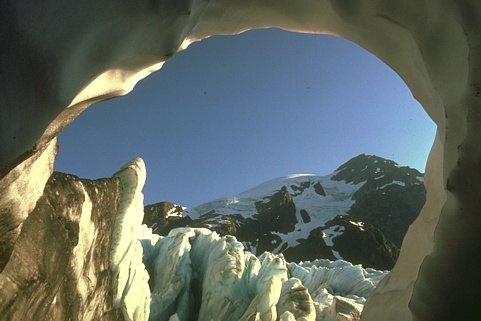
\includegraphics[width=1\linewidth]{figures/img/image/176051.jpg}
\end{minipage}}
\hspace{-2.5mm}
\subfigure[图像分割]{
\begin{minipage}[b]{0.3\linewidth}
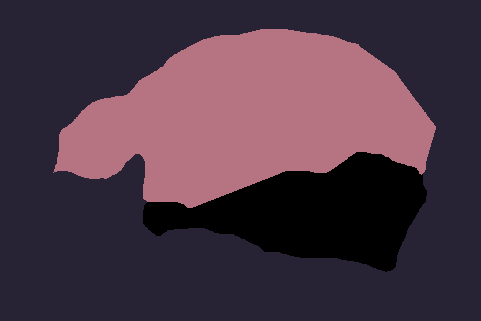
\includegraphics[width=1\linewidth]{figures/img/gt/gt_176051.png}
\end{minipage}}
\hspace{-2.5mm}
\subfigure[超像素分割]{
\begin{minipage}[b]{0.3\linewidth}
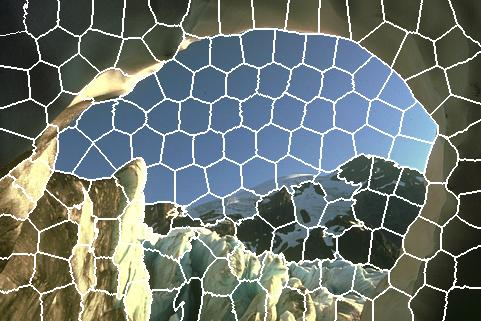
\includegraphics[width=1\linewidth]{figures/img/SLIC/SLIC_176051.jpg}
\end{minipage}}

\caption{图像分割与超像素分割示例}
\label{fig1.1}
\end{figure*}

\section{国内外研究现状}

\subsection{超像素分割算法研究现状}


超像素\cite{ren2003learning}自从在2013年提出之后,研究人员对这一领域做出了很多贡献,并取得了丰富的成果。
本小结对于超像素算法进行简单整理和总结。

1. 基于图论法

该方法的基本思想是将图像映射到对应的加权无向图,无向图中的顶点与图像中的像素一一对应,点与点之间边的权重由像素之间的特征差异性计算得来。
基于图论法就是将加权无向图根据一定的准则划分为数个连通子树,从而得到超像素分割结果。

设$G=(V,E)$表示由$n$个顶点$v\in V$和$m$个边$e\in E\subseteq V\times V$组成的无向图,每个像素与一个顶点相关联。
每个边$e_{ij}=(v_i,v_j)$都被分配了一个权重(通常为非负实值),该权重表示了两个顶点之间的差异值。
超像素分割是将图$G$划分为$k$个独立的分量,$k$表示超像素个数,每个分量对应一个连通子图${G}'=({V}',{E}')$,
其中${V}'\subseteq V$和${E}'\subseteq E$。

Ncut\cite{shi2000normalized}方法自从提出之后,已经发展了多个版本。它将图像映射到加权无向图中,边的权重由纹理特征和轮廓特征差异计算而来。并定义了目标函数,通过最小化目标函数,使得分割出的超像素类间距离尽可能大,并且类内距离尽可能小,从而实现超像素分割。虽然它可以生成规则的超像素,但边界的保持效果并不理想,且计算量较大,速度较慢。

2017年,Chen等提出的实现了线性谱聚类( Linear Spectral Clustering,LSC)\cite{li2015superpixel},
通过从颜色和空间两方面来计算像素之间的相似度,
利用内核相似度度量函数,将图像像素巧妙的映射到高维特征空间中,
通过特征空间的加权K-means\cite{1967Some} 度量优化目标函数。
算法的效率得到了大大提升,且超像素更加均匀致密。

2018年,Xing等人提出Superpixel Hierarchy\cite{SpHierarchy},利用Boruvka\cite{2003Boruvka}算法实现无向图的区域合并。把一个图看成有$n$个树的森林($n$为图像中像素数目),每个顶点看成一棵树。
对于每棵树来说,找到它最近的邻点,即边的权重最小的那个点,并把他们合并在一起。
Boruvka算法重复融合树直到只有一棵树留下来。用Boruvka算法得到最小生成树(MST),同时记录每个边缘的顺序添加到MST。
一旦边缘被添加到MST,森林中的树木数量减少一个。
假设需要提取$k$个超像素,通过前$n-k$个边连接顶点,并且具有$k$ 个连接的组件,这些组件恰好是超像素。

其优点是具有线性时间解,可并行化。此外,该方法在聚类的过程中融入了局部信息,比SLIC和LSC等只利用每像素特征来确定聚类隶属关系的方法更为健壮。

2. 基于梯度下降法

%watersheds,Mean-shift,Quick-shift,Turbopixels,SLIC
简单线性迭代聚类(simple linear iterative clustering,SLIC)作为最经典的超像素分割算法,具有很多优点,计算简单且速度快,可以生成规则的超像素,此外可以控制超像素数量。
但是其生成的超像素边界的保持效果并不理想,而且抗噪性较差。
SLIC将彩色图像转换为CIELAB颜色空间和XY坐标系下的5维特征向量,然后构造5维特征向量的距离度量来对像素进行局部聚类。

zhao等人在SLIC的基础上进行了改进,提出了像素快速线性迭代聚类(Fast Linear Iterative Clustering,FLIC)\cite{Zhao2017FLIC}算法。
FLIC从一个新的角度重新考虑图像的超像素分割问题,利用先验信息,提出了一种名为“Active Search”的新型搜索算法,它明确地考虑了超像素的连通性。
基于这种搜索方法,设计了一个back-and-forth的遍历策略并且合并了SLIC中的分配和更新步骤。
与SLIC相比,FLIC降低了收敛所需的迭代次数,并且提高了超像素分割的边界灵敏度,具有更好的边缘重合度。

3. 基于深度学习的超像素分割算法

近年来,对于广泛的计算机视觉问题采用深度学习的情况急剧增加,但超像素几乎不与深度学习和神经网络结合使用。
这有两个主要原因。首先,标准卷积运算通常定义在规则网格上,当在不规则超像素网格上操作时变得不合适。
其次,现有的超像素算法是不可微的,因此如果在神经网络中使用超像素,
就会在其他端到端可训练网络架构中引入了不可微的模块。

2018年,Varun Jampani等人提出了一种基于深度学习的聚类算法Superpixel Sampling Networks(SSN)\citep{jampani2018superpixel},通过放宽SLIC中存在的最近邻约束将其转化为可微算法。
这种新的可微算法允许端到端训练,从而能够利用强大的深层网络来学习超像素。
其优点包括:端到端可训练,可以轻松集成到其他深层网络架构中;速度快,可以生成边界保持度高的超像素。


\subsection{图像分割研究现状}

(1) 特征空间聚类法

图像分割根据灰度、彩色、空间纹理、几何形状等特征把图像划分成若干个互不相交的区域,
使得这些特征在同一区域内表现出一致性或相似性,而在不同区域间表现出明显的不同。
因此,可以将图像分割问题以像素的分类问题来解决。
同类的像素在灰度、彩色、空间纹理等方面具有较高的相似性,而不同类中的像素间差异比较大。

特征空间聚类法作为无监督的图像分割算法,可以减少人为干预,自动完成分割。
但一般需要提前确定分类数,然后通过迭代地来提取各类的特征值,来执行分类算法,
更新聚类中心,例如K-均值\cite{comaniciu2002mean},Fuzzy C-means (FCM)\cite{zaixin2013neighbourhood,gong2012fuzzy,zhang2017novel} 聚类算法等。

特征空间聚类作为已经很成熟的算法,有很多优点,例如:不需要训练样本,方法简单,方便执行。
也有相应的缺点:分类数一般很难确定,且初始参数对最终结果有较大的影响。
此外,特征空间聚类没有充分利用像素之间的局部信息,一般只是采用空间或颜色特征,从而对噪声比较敏感。

(2) 边缘检测法

所谓的图像边缘,即在一张图像中,两个不同区域的交界处,图像中相邻区域交界处的像素结果组成了图像的边缘。
根据经验,沿着边缘走向,像素值变化较为平缓;而垂直于边缘,像素值变化较大。
因此,可以将图像中灰度发生突变的像素看为边缘。

边缘检测的基本思路一般为:先根据一定的算法来确定图像中的边缘像素集合,目前边缘检测方法来得到边缘像素集合的方法,最实用也最简单方法就是构造边缘算子。采用何种边缘算子来提取图像边缘是边缘检测方法的核心问题。
常见的边缘算子有Roberts,Sobel,PreWitt和Carry等。
边缘检测得到的结果还需要进一步处理,如边缘跟踪,边缘松弛法,将边缘像素连接成图像轮廓,得到图像分割结果。


对于噪声比较小的图像,即图像中的不同区域差别明显,边缘检测方法可以取得较好的结果。若图像比较复杂,且不同区域间的差别不是特别明显,则会产生很多噪声。其难点在于确定边缘时,抗噪性和精确度的矛盾。
若抗噪性提高,就会产生位置偏差或轮廓漏检。若提高边缘精确度,那么噪声就会产生不合理的伪边缘。

(3) 基于区域的方法

类似于边缘检测法,区域分割法利用了图像中局部区域的一致性,直接按照一定的一致性判断来寻找分区,分区内的像素具有相似的性质,最终得到图像分割结果。其中的一致性判断包括:灰度、色彩、纹理、形状等。
基于区域的图像分割大致可以分为两大类:区域生长法,区域分裂与合并。

区域生长法的关键核心在于选取或制定合理的生长准则,按照一定的生长准则将像素或子区域合并成更大的区域。
生长准则可以按照不用的判断标准来制定,基本使用图像的局部信息来制定,如基于灰度级类似准则,基于颜色相似准则,基于纹理相似准则等。
不同的生长准则会影响分割过程,从而对最终的分割结果造成影响。
区域生长法最主要的优点就是计算简单,适合于分割小的结构。但其对噪声敏感,抗噪性弱,导致分区中有空洞。

区域分裂与合并算法的基本思路类似于微分,即无穷分割,然后将分割后满足相似度准则的区域进行合并。
四叉树分解法作为典型的区域分裂合并,应用广泛。我们以灰度级作为分裂合并准则,则基本的分裂与合并算法为:首先对于图像中灰度级不同的区域,均分为4 个子区域;若相邻的子区域所有像素的灰度级相同,则将其合并;重复前面两个步骤,直到不再有新的分裂与合并为止,从而得到最终的分割结果。

区域生长算法和区域分裂合并算法作为基于区域的分割方法,在实际应用中经常结合使用,以取得更好的结果。
该类算法对某些复杂物体定义的复杂场景的分割或者对某些自然景物的分割等类似先验知识不足的图像分割,效果较为理想。

\subsection{利用超像素进行图像分割研究现状}

通过学习像素或超像素的相似性进行分割也是一种趋势\cite{chaibou2019learning}。Ahn和Kwak\cite{ahn2018learning}提出了仿射网来预测一对相邻图像坐标之间的语义一致
性。利用仿射网预测的邻接词,通过随机游动实现语义传播。基于超像素描述子
向量之间的距离度量来计算超像素相似度,Chaibou等人\cite{carpineto2012consensus} 引入了一种
新的超像素上下文描述器来增强学习特征,以更好地进行相似性预测。然后通过
迭代合并使用相似性加权目标函数选择的最相似的超像素对来实现图像分割。


超像素池网络(Superpixel Pooling Network,SPN)\cite{kwak2017weakly}提出的超像素池化操作为超像素特征提取提供了新思路。SPN 利用输入图像的超像素分割作为一个池化布局来反映底层图像结构,用于学习和推断语义分割。

deep embedding learning(DEL)\cite{liu2018deep}算法利用超像素池运算提取超像素特征进行图像分割,取得了良好的效果。在提取的超像素的基础上,利用超像素池运算提取超像素的特征来计算超像素的相似度。根据相似度来判断超像素是否进行合并,从而得到最终的分割结果。

2018年,Tao Lei等人提出了superpixel-based fast FCM(SFFCM)\cite{liu2018deep},其算法通过多尺度形态梯度重建(multiscale morphological gradient reconstruction,MMGR)和分水岭变换(watershed transform,WT)获得超像素,然后利用基于超像素的SFFCM 进行图像分割。
与其他聚类算法相比,该算法耗时更少。然而,聚类中心的初始值难以确定,不能得到广泛的应用。


\section{论文研究内容和结构安排}

\subsection{论文研究内容}

本文的主要研究内容是计算机视觉中两个主要的方向-超像素分割,图像分割。虽然现在有很多优秀且成熟的算法来实现超像素分割或者图像分割,但也存在一些问题:首先现在的神经网络没有将超像素分割和图像分割两个任务有效的结合起来,只有部分算法将现有的超像素作为图像分割的输入进行计算。其次,现有的超像素算法基本还是以传统算法为主,并没有真正与神经网络结合起来,发挥神经网络的优势。此外,图像分割算法还是基本以像素为单位进行运算,并没有引入超像素进入有效的计算。

针对此问题,本文提出了端到端的可训练网络,可以同时产生超像素和进行图像分割。
使用完全卷积网络和迭代可微聚类算法来获得超像素。
接下来,采用超像素池层来获得超像素特征,并以此计算相邻超像素之间的相似度。
如果相似度大于预先设定的阈值,则通过简单的步骤将其合并,得到目标片段。
本文在使用BSDS500数据集\cite{arbelaez2010contour}上,最先进的结果进行多次使用比较,结果验证了本文方法的有效性和可行性,
实现了精细的超像素分割和图像分割。

此外,本文还提出了基于Boruvka算法和快速模糊C均值聚类的图像分割方法。
该方法首先使用一种基于Boruvka算法来产生超像素图像。
在Boruvka算法获得的超像素图像的基础上,通过计算超像素图像的颜色直
方图来实现快速模糊C均值聚类算法,实现彩色图像的快速分割。

\subsection{论文结构安排}

本文结构安排如下:

第1章为绪论,介绍了超像素和图像分割的基本概念,并分类介绍了超像素分割和图像分割的经典方法,
最后简要介绍了本文。

第2章首先简介了深度学习和神经网络理论,然后详细介绍了卷积神经网络基本理论,此外详细介绍了像素分割和图像分割的经典方法,最后介绍了超像素池化方法。

第3章首先回顾了经典的SLIC方法的核心步骤,然后介绍了基于深度学习的超像素分割和图像分割方法。

第4章基于Boruvka算法和快速模糊C均值聚类的图像分割方法。

第5章首先说明本文实验中的公开数据集及评定标准,然后基于第3章和第4章的方法进行消融实验,
最后对本文介绍的算法与已有的先进算法进行对比实验并分析结果。

第6章对全文进行总结,并在本文工作的基础上,对进一步的工作进行了展望。

%\clearpage{\pagestyle{empty}\cleardoublepage}
% !Mode:: "TeX:UTF-8"

\chapter{超像素分割和图像分割理论基础}

本文第1章介绍了超像素和图像分割的基本概念,并分类介绍了超像素分割和图像分割的研究背景及研究现状。
在本章中将对相关的基本理论进行简要的介绍。
首先简要叙述深度学习和神经网络的相关理论研究,接着介绍经典的基于神经网络的图像分割方法。
然后简述超像素在图像分割的意义。此外,介绍了将超像素整合到神经网络中的理论基础-超像素池化层。

\section{深度学习}
\begin{figure*}[h]
\begin{center}
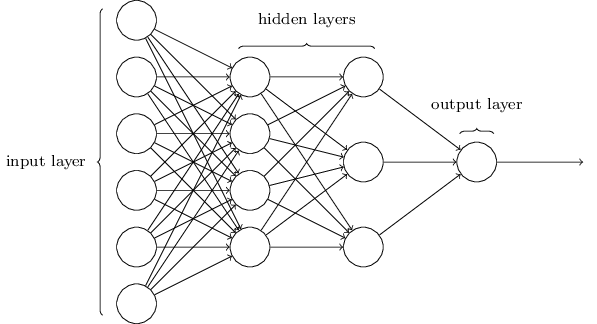
\includegraphics[width=1\textwidth]{figures/CNN0.png}
\end{center}
\vspace{-5mm}
\caption{多层感知器示意图}
\end{figure*}
%概念,分类,
2016年3月,在中央发表的"十三五"规划纲要中,“人工智能”一词格外引人注目。
BAT等各大互联网公司对人工智能领域的投入更是将人工智能这一领域的发展推向一个新的高潮。
目前深度学习无疑是人工智能的重点研究领域之一,设计到人工智能众多领域,如计算机视觉、自然语言处理等。

%浅层区别  《深度学习研究综述》
深度学习其实是机器学习的一种,从最初的浅层机器学习发展到目前深度学习。与浅层机器学习相比,深度学习加深了模型结构深度,一般有5 层,6 层,甚至更多的隐层节点。
一般而言,随着深度的增加,模型的学习能力也在增加。
此外,深度学习是一种特征学习,能够利用大数据来学习特征,从而能够获取数据更高层次的抽象表示,来描述数据的内在信息。

深度学习的概念源于人工神经网络的研究,深度学习网络最基本的结构是多层感知器(multilayer perception,MLP)。多层感知器,也就是我们所说的前向传播网络,一般有多层构成,每一层由若干神经元组成,如图2-1所示。



如图2-2所示,对于第$l$层,多层感知器的前向传播公式如下:
\begin{equation}
y_{i}^{k+1} = \sum_{j}W_{k}^{ij}y_{j}^{k}+b_{i}^{k}
\end{equation}
其中,$y_{j}^{k}$表示第k层的第j个神经元的输出,
$W_{k}^{ij}$表示第k层中第j个神经元与第k+1层的第i个神经元之间的权重,$b_{i}^{k}$是偏置值。
通常进行完这一步之后,会在此基础上使用非线性激活函数进行激活运算,常见的激活函数有ReLU、Sigmoid等。

\begin{figure*}[h]
\begin{center}
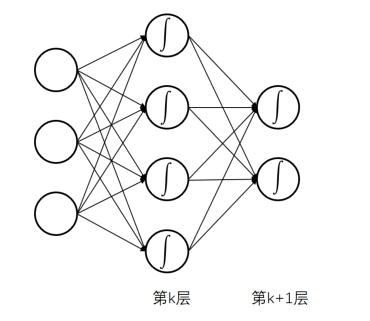
\includegraphics[width=1\textwidth]{figures/CNN01.png}
\end{center}
\vspace{-5mm}
\caption{前向传播示意图}
\end{figure*}
%应用
由于理论和计算力的原因,深度学习从提出到本世纪出,深度学习一度被边缘化,成果泛善可陈,直到2012年ImageNet比赛,多伦多大学团队开发的AlexNet模型的出现,以卷积神经网络( convolutional neural network)为基础,识别效果超过了所有浅层的方法。从此开启了深度学习进入快速发展的新时期,已经被广泛应用到计算机视觉、语言识别、自然语言处理等领域。

2015年的世界大规模人脸识别竞赛LFW中,来着香港中文大学多媒体实验室的中国团队使用深度学习模型,打败FaceBook 团队获得冠军。是的在人脸识别领域,深度学习的识别能力穿越真人。
此外在计算机视觉领域中的行人检测、多人姿态估计、物体跟踪、场景识别、图像分类、图像分割、物体跟踪等都有深度学习的身影。
近年来,科研人员也将深度学习应用到很多有意思的方向,例如:去除马赛克、风格迁移、黑白照片自动上色、图片补全等。

深度学习虽然很早应用于计算机视觉,在语音处理领域最先取得突破性进展。语音处理主要分为语音识别和语音合成两大方向。2016 年,微软利用深度学习开发的语言识别模型,在日常对话识别准确度上首先达到了人类水平,真正让大家大吃一惊。此外,各大公司也都在研究利用深度学习来进行语言合成,并已有成熟的系统,例如谷歌的WaveNet模型,百度的Deep Voice3。

2013年,Tomas Mikolov等人发表论文《Efficient Estimation of Word Representations in Vector Space》,提出了word2vector 模型,这也是目前自然语言处理通常使用的模型,与传统的词袋模型(bag of words)相比,word2vector能够更好地表达语法信息。
目前深度学习在自然语言处理领域的应用主要包括:问答系统、情感分析、机器翻译、句子成分分析等。
\section{卷积神经网络}

%定义
简单来说,卷积神经网络(Convolutional Neural Networks)是深度学习模型中的其中一类,类似于人工神经网络的多层感知器。
Yann LeCun在1994年提出的LeNet模型,最早将CNN应用于数字识别。2012年,多伦多大学Alex Krizhevsky等人开发的AlexNet模型第一次让大家注意到了CNN的强大之处。

% 网络结构
LeNet模型只有卷积层和池化层,全连接层,后来AlexNet模型在此基础上,加入了Relu激励层,提高了效率。接下来会分别介绍相关理论和计算。

\subsection{卷积层}
% 卷积操作
\begin{figure*}[h]
\begin{center}
%\fbox{\rule{0pt}{2in} \rule{.9\linewidth}{0pt}}
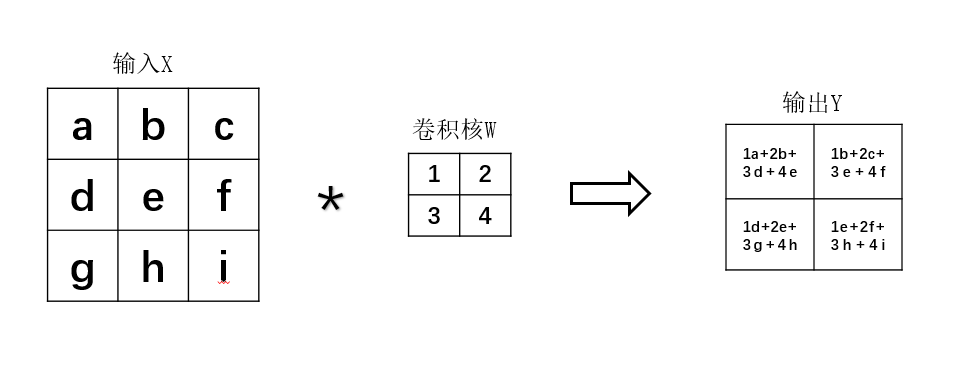
\includegraphics[width=1\textwidth]{figures/CNN1.png}
\end{center}
\vspace{-5mm}
\caption{卷积计算过程示意图}
\end{figure*}

卷积层作为卷积神经网络最重要的一层,其作用主要是提取图像的局部特征。如图2-2所示,卷积层的卷积操作为卷积核W与输入矩阵X 进行从左到右从上到下,步长为1的相乘相加操作,得出输出Y。卷积核W的大小为$M_w x N_w$,输入矩阵的大小为$M_x x N_x$,那么输出矩阵的大小等于$(M_x-M_w+1)x(N_x-N_w+1)$。
以图2-3为例,一个3x3的卷积核在一个5x5的输入图像上以步长为1做卷积计算,得到3x3的输出矩阵,这个输出矩阵就是特征矩阵。

\begin{figure*}[h]
\begin{center}
%\fbox{\rule{0pt}{2in} \rule{.9\linewidth}{0pt}}
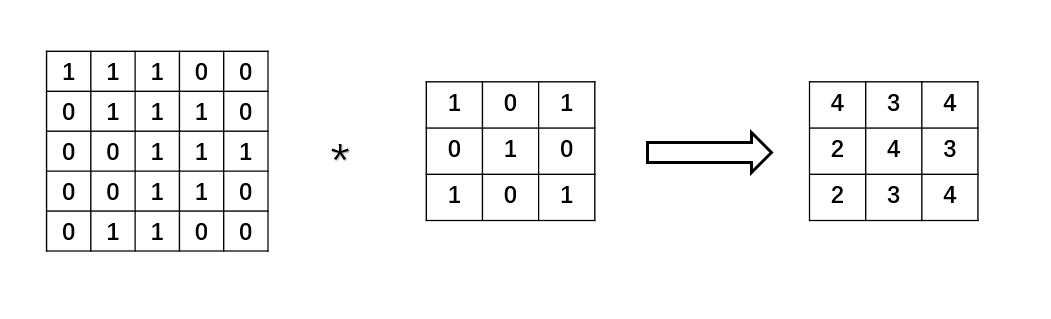
\includegraphics[width=1\textwidth]{figures/CNN2.png}
\end{center}
\vspace{-5mm}
\caption{卷积操作示意图}
\end{figure*}

\subsection{激活层}
%Relu激活
最原始的感知机(perceptron)并没有激活层,无论有多少层神经网络,输出层的结都是输入数据的线性组合,不能满足解决神经网络复杂任务的需求。因而加入了激活层,使用非线性函数作为激活函数,使得深层神经网络有了学习的能力,可以逼近任何函数。

用sigmoid函数和tanh函数作为最初的激活函数,输出有界,很容易充当下一层的输入。
随着神经网络的深度增加,卷积神经网络在反向传播过程中存在梯度消失的问题,
Sigmoid等激活函数的导数很小,而连续多个很小的数,结果几乎为0,因此梯度无法从输出层传到输入层。随着神经网络的深度增加会造成梯度消失的问题,从而导致训练难度大,效果不佳。此外,反向传播求梯度时,Sigmoid函数计算量较大。

2012年提出的AlexNet引入了一种新的激活函数-ReLU函数。该函数的提出很大程度的解决了BP算法在优化深层神经网络时的梯度耗散问题,而且减少了计算量。此外,Relu会使一部分神经元的输出为0,这样就造成了网络的稀疏性,并且减少了参数的相互依存关系,缓解了过拟合问题的发生。

现在也有一些对relu的改进,比如prelu,random relu等,对于不同的任务上,准确率或速度上有一定的改进。
此外,现在卷积神经网络,一般会在Relu激活层之后会多做一步归一化操作,尽可能保证每一层网络的输入具有相同的分布,减少计算量。

\subsection{池化层}
% 池化操作
在连续的卷积层之间一般会放入池化层,其目的是压缩数据,降低维度,减少计算。
池化层用的方法包括最大池化(Max pooling)和平均池化(Average pooling)。以最大池化为例,如图2-3所示,在一个4*4的矩阵上,选用2*2的filters,步长为2,对于每个2 * 2 的窗口选出最大的数作为输出矩阵的相应元素的值,比如输入矩阵第一个2 * 2窗口中最大的数是6,那么输出矩阵的第一个元素就是6,如此类推。平均池化的原理类似,只不过输出矩阵中的元素是输入矩阵对应窗口中元素的平均值。
\begin{figure*}[h]
\begin{center}
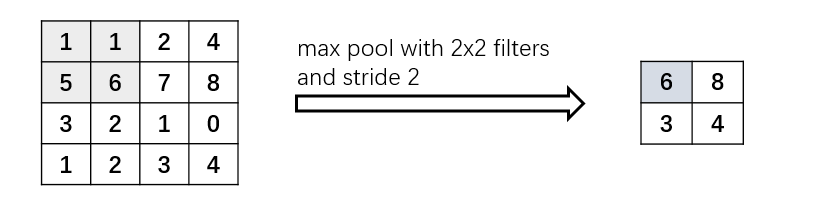
\includegraphics[width=1\textwidth]{figures/CNN3.png}
\end{center}
\vspace{-5mm}
\caption{池化操作示意图}
\end{figure*}

接下来具体介绍池化层的具体作用。如果输入数据是一张图片,那么池化层的作用就是对图像进行压缩。压缩过程中,去掉一些无关紧要的特征信息,留下最能体现图像特征的信息。我们知道,一张图像中含有的很多的信息,也具有很多的特征,但是有些特征信息,对于需要完成的任务则显得无关紧要,过于冗余。池化操作就是要去除这些冗余信息,留下最重要的特征信息。

池化操作具有特征不变性。所谓的特征不变性就是一张狗的图像被缩小了一倍,但还能认出这是一张狗的照片。
这说明在压缩过程中只是去除了无关紧要的信息,但对狗的重要特征信息仍有保留,因此我们依然可以能判断出这是一只狗。
% 发展
批归一化(Batch Normalization,BN)是深度学习发展中的一个里程碑式的技术,使各种网络能够进行训练。
在卷积神经网络训练过程中,由于参数是不断更新的,随着网络层数的加深,对于深层网络,其输入数值不稳定,导致模型很难收敛。通过归一化,对中间层的输出结果进行标准化处理,使得其更加稳定,分布更加固定,有利于算法的稳定和收敛。

然而,沿着批处理维度进行规范化会带来问题——当批处理大小变小时,BN的错误会迅速增加,这是由于批次统计估计不准确造成的。2018年,Yuxin Wu提出了Group Normalization,GN将通道分成组,并计算每组中的均值和方差进行归一化。GN的计算与批量大小无关,更适合于批次较小的任务。

\section{基于神经网络的图像分割}
《基于深度学习的RGB-D图像语义分割》
《FCN》http://www.sjocr.com/news/915.html
\section{超像素在图像分割中的意义}
%《基于图论的超像素分割及合并算法》
对于图像分割任务,基于像素的传统处理方法取得了不错的成果。
但是随着数码产品的拍照功能迅速发展,图像的构成越来越复杂,分辨率不断增大,越来越清晰,包括的像素数量也是成指数级增长。
在这样的背景下,基于像素的传统图像分割方法处理分辨率高的图像,将花费更多的时间。

如何减少图像分割的计算量显得尤为重要。超像素作为一种图像预处理技术解决了这个问题。
所谓超像素,就是由局部的许多像素构成的区域,这些区域内的像素通常由具有相似纹理、颜色、亮度等特征。
相对于像素而言,超像素不仅有效减少了局部的冗余信息,后续处理过程中的计算量和复杂度大幅度降低,而且更利于局部特征的提取与表达,更有利于帮助定位区域的边界。

\section{超像素池化层}

2017年,Suha Kwak等人提出了Superpixel Pooling Network (SPN)网络,将超像素分割结果作为低阶结构的表征,利用提出的超像素池化层对输入网络的超像素进行提取特征,辅助语义分割的推断。
此外,SPN网络验证了使用了Superpixel可以提高图像分割的准确率,确实能起到一定的效果。

在这里简单介绍一下SPN网络中超像素池化层的具体操作,每个超像素的特征向量生成如公式2-2所示:
假设 $P_{i}= \left \{ p_{i}^{k} \right \} k=1,2,\cdots ,K_i$ 表示图像中第i个Superpixel,$K_i$表示第i个Superpixel 中像素的个数,对于每个Superpixel i,feature vector 的生成公式:

\begin{equation}
v_{i} = \frac{1}{K_i}\sum_{j}\sum_{k}I(p_{i}^{k}\in r^{j})z^{j}
\end{equation}
其中,$r^{j}$表示感受野, $z^{j}$表示经过上采样得到的特征图中的第j个位置的值。 $I(p_{i}^{k}\in r^{j})$是一个indicator 函数,如果括号中的值为true,则返回1,否则返回0。

固定当前某一个超像素,将之池化。式中的$r$存在是因为存在尺度差异,是感受野大小。
作者的池化方式是固定超像素,遍历特征图和超像素内的元素,计算当前超像素元素在位置j感受野所占的比例,然后加权上去。
通过式2-2便可以得到每个超像素的特征向量,从而可进行后续的运算。

%\clearpage{\pagestyle{empty}\cleardoublepage}
% !Mode:: "TeX:UTF-8"

\chapter{基于深度学习的超像素分割和图像分割}

\begin{figure*}[h]
\begin{center}
%\fbox{\rule{0pt}{2in} \rule{.9\linewidth}{0pt}}
\includegraphics[width=1\textwidth]{figures/img/pipeline.pdf}
\end{center}
\vspace{-5mm}
\caption{算法流程图。对于给定的图像,我们的算法同时生成超像素和图像分割。输入图像首先被输送到一个特征提取网络,该网络由一系列卷积层、归一化(GN)和ReLU操作组成。然后将提取的特征输入可微聚类模块,生成超像素。超像素池用于获取超像素特征向量。最后通过合并相似度高的超像素实现图像分割}
\label{Fig.sub.1}
\end{figure*}

如图3-1所示,我们的方法首先从CNN深度网络中学习图像特征,然后我们使用迭代可微分聚类算法模块来获取超像素。接下来,我们通过超像素池化层计算超像素特征向量,并计算相邻超像素之间的相似性。最后,根据相似度判断相邻的两个超像素是否合并。在本节中,我们将详细介绍我们的方法。

\section{超像素生成}

超像素将相似像素分组为各向同性区域,从而可以提高分割质量和效率。 例如,在DEL算法中,作者使用SLIC作为图像分割的开始。在本文中,与采用现有的超像素算法进行图像分割的方法不同,我们将超像素生成作为图像分割网络的一部分。为此,我们采用SSN中提出的可微聚类算法模块,以取代SLIC算法中的硬像素-超像素关联。

通常,对于$n$像素的图像\(I\in\mathbb{R}^{n\times 5}\),在CIELAB空间的特征为$I_p=[x,y,l,a,b]$ ,我们希望将其划分为$m$ 个小区域,即将图片分成m个超像素。在介绍在描述软关联之前,我们简要介绍SLIC算法中如何计算像素-超像素硬关联$H = \left \{1, 2, \cdots, m \right \}^{n\times 1}$。给定统一采样的超像素中心$C^{0}$作为初始值,SLIC算法在每次迭代$t$中计算每个像素$p$处的新超像素分配,
\begin{equation}\label{eqn:hardassn}
H_{p}^{t} =  \mathop{{{\rm argmin}}}\limits_{{i\in\{ 1, 2, \cdots ,m \} }}\left\|I_{p}-C_{i}^{t-1}\right\|_2,
\end{equation}
其中$\|\cdot\|_2$表示输入向量的$\ell_2$范数,$C_i^{t-1}$表示超像素中心$i$的特征,该特征通过对第$t$次迭代后,计算属于该超像素中心的像素的特征平均值来获取。

由于(3-1)获取像素-超像素硬关联H的操作是不可微的,因此SLIC无法直接集成到神经网络中。 在我们算法中的用到的可微分聚类算法模块,其将硬像素-超像素硬关联H替换为软关联Q。与原始SLIC相似,它在每次迭代中具有以下两个核心步骤:

1.	像素-超像素关联计算。第t次迭代中像素p及其相邻超像素i之间的关联计算如下:
\begin{equation}
Q_{pi}^{t} = e^{-\left \| F_{p}-C_{i}^{t-1}\right \|_2^2},
\end{equation}
其中\(F_{p}\)是像素$p$的深层特征。 在我们的情况下,它来自我们网络的特征提取模块。\(Q_{pi}^{t}\)是$t$次迭代后像素$p$与超像素中心$i$之间的距离。

2.	超像素中心更新。新的超像素聚类中心是根据像素特征的加权总和得出的,
\begin{equation}
C_{i}^{t} = \frac{1}{Z_{i}^{t}}\sum_{p}Q_{pi}^{t}F_{p},
\end{equation}
其中$Z_{i}^{t}$表示归一化过程,即$Z_{i}^{t} = \sum\nolimits_{p}Q_{pi}^{t} $ 。

将这两个步骤迭代数次(在本文中,设定迭代次数为10次),最终得到像素-超像素软关联\(Q\in\mathbb{R}^{n\times m}\)。与(3-1)相似,我们需要计算硬关联映射$H'\in \mathbb{R}^{n\times 1}$,最终得到像素$p$的超像素标签,
\begin{equation}
H'_{p} =  \mathop{{{\rm argmax}}}\limits_{{i \in \left\{ 1, \cdots ,m \right\} }}Q_{pi}.
\label{equation.3}
\end{equation}

值得注意的是,这种硬关联的计算是不可微的。因此在我们的算法中,这一步不参与反向传播。在实验中,我们发现计算像素和超像素聚类中心之间的软关联非常耗时。与SLIC相似,我们只是计算每个像素到周围超像素聚类中心的距离,大大减少了计算时间。

\section{超像素相似度}
在获得超像素之后,我们需要测量它们之间的相似性。超像素的特征可以用超像素池来计算,它实际上是计算属于某个超像素的像素特征的平均值。在我们的算法中,当执行超像素池时,我们使用了不同于在超像素生成中使用的像素特征,如图3-1所示,使用浅蓝色矩形所表示的图像特征。其背后的原因是,超像素不包含语义信息,而图像分割却包含语义信息,因此这两种任务的特征是不同的。我们在实验中通过比较超像素和图像分割的结果以及该算法的一个变体(ours-conv7)来验证这一思想。参考第4.1了解更多细节。

获取超像素后,我们假设超像素的数量为M,将超像素集合表示为$\mathcal{S}=\{S_{1},S_{2},\cdots ,S_{m}\}$,根据图3-1所示,我们所得到的超像素进行超像素池化操作,得到对应超像素的特征向量$\{ v_{1},v_{2},\cdots,v_{m}\}$。超像素池化操作表示如下:
\begin{equation}
v_{i} = \frac{1}{|S_{i}|}\sum_{p\in S_{i} }F'_{p},
\end{equation}
其中,$F'_{p}$ 表示在超像素池中使用的像素$p$的特征向量。

相邻超像素i和超像素j的相似度可以由如下公式获得:
\begin{equation}\label{eqn:sim}
s_{ij} = \frac{2}{1+{\rm exp}\left ( \left \| v_{i}-v_{j}\right \|_{1}\right )},
\end{equation}

其中$s_{ij}$的范围是$[0,1]$。$s_{ij}$值越大,超像素$i$和$j$的相似性越高。当$v_{i}$和$v_{j}$非常相似时,$s_{ij}$接近1,相反,当$v_{i}$和$v_{j}$极为不同时,它接近于0。我们根据相似度$s_{ij}$决定是否合并超像素$i$和$j$。

\section{损失函数}

我们假设同一分割区域内的超像素对之间的相似性大于不同分割区域中的超像素对的相似性。基于(3-6)中定义的相似性度量,我们定义的损失函数如下:
\begin{equation}
\begin{split}
 L =  - \sum_{S_{i}\in S}\sum_{S_{j}\in \mathcal{R}_{i}}   \left[   { \left(
 1  -\alpha  \right)\cdot l_{ij}\cdot \log \left( s_{ij} \right)  } \right. \\
 \left. {  + \alpha \cdot \left( 1-l_{ij}\right) \cdot \log \left( 1- s_{ij}\right)  }   \right],
 \label{equation.6}
\end{split}
\end{equation}
其中$\mathcal{R}_{i}$是超像素$S_{i}$的相邻的超像素集合,$S_i$表示$S_i$和$S_j$是否属于同一个分割区域。在实际应用中,$l_{ij}$ 是由所获得的超像素集和数据集提供的真值来计算的。在$S_i$和$S_i$属于同一分割区域的情况下,$l_{ij} = 1$;否则,$l_{ij} = 0$。

注意,对于不同的输入图像,$l_{ij}$ 的矩阵是不同的。因此,训练阶段的小批量大小必须设置为1,即一次只向网络中输入一张图像。参数$\alpha$表示在真值中属于同一区域的超像素对的比例,用于平衡正样本和负样品。通过将$|Y_+|$ 表示为属于同一区域的超像素对的数目,将$|Y|$表示为超级像素对的总数,通过$\alpha  = \left | Y_{+}\right | / \left | Y \right |$ 来计算。通过反向传播,图像分割也指导了超像素分割。

\section{超像素融合}

通过合并相似的超像素得到最终的图像分割。我们利用相邻超像素之间的相似性和一个预先设定的阈值T来确定两个相邻超像素是否合并。算法1概述了超像素合并的计算步骤。
\begin{algorithm}[h]
  \caption{Superpixel merging algorithm}
  \textbf{Input}: $s$ : similarity;
  \hspace*{2em} $T$ : similarity threshold;\\
  \hspace*{2.5em} $\mathcal{S}=\{S_{1}, S_{2},\cdots, S_{m}\}$ : superpixels.\\
  \textbf{Output}: Segmentation $\mathcal{S}$.
  \begin{algorithmic}[1]
    \For{each $S_{i}\in \mathcal{S}$}
    \State Construct adjacent superpixel set $\mathcal{R}_{i}\subset \mathcal{S}$ of $S_i$;
        \For{each $S_{j}\in R_{i}$}
            \If {$s_{ij} > T$}
                \State$S_{i} \gets S_{i}\cup S_{j}$, $\mathcal{S} \gets \mathcal{S} \setminus S_{j}$ ;
                \State Update $\mathcal{R}_i$ ;
            \EndIf
        \EndFor
    \EndFor
    \label{algorithm1}
  \end{algorithmic}
\end{algorithm}

\section{网络结构}

图3-1显示了我们的网络结构。用于特征提取的CNN网络由卷积层、组规范化(GN)和ReLU激活函数组成。我们将GN中的组数设置为8。在第2层和第4层卷积后,我们使用最大池来增加感受野。对第4层和第6层的输出进行采样,然后与第2层的输出连接,以丰富提取的特征。我们使用3$\times $3卷积滤波器将输出通道设置为每层64个。

注意,考虑到网络中每个小批量的大小必须为1,我们用GN替换了广泛使用的批处理规范化(BN)层。BN操作是深度学习发展中的一个里程碑式的技术,使各种网络能够进行训练。然而,沿着批处理维度进行规范化会带来问题——当批处理大小变小时,BN的错误会迅速增加,这是由于批次统计估计不准确造成的。相反,GN将通道分成组,并计算每组中的均值和方差进行归一化。GN的计算是独立于批量大小的,其精度在较大的批量范围内是稳定的。在实验中,我们还比较了用BN和GN作为归一化的结果。

在多任务学习中,不同层次的任务需要不同的图像特征,如supernet。对于超像素生成和图像分割这两个不同层次的任务,我们进一步对上一步得到的图像特征进行卷积运算,得到不同的特征向量,以满足不同任务的需要。具体来说,对于超像素生成任务,我们使用核大小为3$\times $3的卷积层来获得30个通道的特征向量。对于图像分割任务,我们首先对256个输出通道进行3$\times $3卷积运算,然后使用1$\times $1卷积核得到64个通道的特征向量。如图3-1所示,我们将得到的特征向量分别输入到后续的可微聚类算法模块和超像素池层,然后利用所提出的相应的损失函数对网络进行训练。

\section{实施细节}

我们基于Caffe框架来搭建神经网络,这是一个非常有效的深度学习框架,广泛应用于学术界和工业界。所有代码都是用C++和Python包装编写的。

对于超级像素的生成,就像在原始的SLIC算法中一样,我们在(3-4)之后的每个超级像素簇内的像素之间加强空间连通性。通过将小于某个阈值的超像素与周围的超级像素合并,然后为每个空间连接的组件分配一个唯一的聚类ID来实现的。对于图像分割,我们在合并后进行空间连通性增强操作。需要注意的是,加强空间连通性的运算是不可微的,我们只把它当作后处理,而不加入神经网络。

我们使用BSDS500数据集作为我们的训练和测试数据,该数据集已在图像分割领域得到广泛应用。由于BSDS500中训练样本数量较少,训练时需要进行数据扩充。我们将每一个真值作为一个单独的样本,即对于每一对图像和真值,我们将其作为训练样本提供给网络。通过这种方式,我们得到了1633对训练/验证对和1063对测试对。另外,我们采用了两种常用的数据扩充策略,即翻转和裁剪。具体地说,在训练阶段,我们将图像左右翻转,随机地将图像裁剪成201$\times $201大小的图像块,进行数据增强。采用Adam优化我们的网络。基本学习率设置为1e-5,生成的超级像素数设置为100。动量设置为0.99,以在相对较小规模的数据上实现稳定优化,如FCN 中所建议的那样。如第3.5,每个小批量的大小设置为1。

我们进行500K次迭代来训练深度学习模型,并根据验证的准确性选择最终的训练模型。


%\clearpage{\pagestyle{empty}\cleardoublepage}
% !Mode:: "TeX:UTF-8"

\chapter{基于超像素的Fast Fuzzy C-Means Clustering在图像分割中的应用}
在这项工作中,我们使用一种基于Boruvka算法来产生超像素图像。Boruvka算法具有线性时间解,可并行化。此外,通过Boruvka 算法,邻里信息可以纳入一个统一的框架。在每次迭代之后,特征在新形成的集群中聚合。这种方法比SLIC和LSC等只利用每像素特征来确定聚类隶属关系的方法更为健壮。

在Boruvka算法获得的超像素图像的基础上,通过计算超像素图像的直方图来实现快速FCM算法。由于超像素图像中不同颜色的数目远小于原始彩色图像,因此计算超像素图像的直方图非常容易。最后,以直方图作为目标函数的参数,实现彩色图像的快速分割。我们提出的算法的框架如图1所示。

\section{通过Boruvka算法生成超像素}

把一个图看成有n个树的森林,每个顶点看成一棵树。
对于每棵树来说,我们找到它最近的邻点,即边的权重最小的那个点,并把他们合并在一起。
假设$C_{2}$是$C_{1}$的最小的邻点($C_{1}$也许并不是$C_{2}$最小的邻点),我们定义两个树之间的距离为:
\begin{equation}\label{eqn:hardassn}
D(C_{1},C_{2}) = \min_{v_{i}\in C_{1},v_{j}\in C_{2},(v_{i},v_{j})\in \varepsilon} \omega ((v_{i},v_{j}))
\end{equation}

最近邻点选择之后,构建辅助图,其中每个顶点表示一个簇,每个边对应一个选定的权重最小的边。如果这里有多个最近的邻点,我们在辅助图上用重复的边来表示他们。另一方面,辅助图上的边是不同的。用深度优先搜索找到连通图。Boruvka算法重复融合树直到只有一棵树留下来。我们用Boruvka算法生成一个最小生成树(MST),同时记录每个边缘的顺序添加到MST。一旦边缘被添加到MST,森林中的树木数量减少一个。假设需要提取k个超像素,我们通过前n -k个边连接顶点,并且具有k个连接的组件,这些组件恰好是超像素。

Boruvka和Kruskal算法之间的主要区别在于前者是局部和并发搜索边缘,而后者在全局范围内对边缘进行排序并按顺序执行。因此,Boruvka算法可以并行处理。此外,Boruvka算法假设簇是均匀分布的,并缓解了Kruskal算法倾向于生成严重不平衡簇的缺点。 在所提出的超像素层次方法中,我们采用Boruvka算法来构造MST。同时,记录每条边加入MST的顺序。一旦将一条边添加到MST中,森林中的树数将减少一棵。假设需要提取k个超像素,我们通过第一个n-k条边连接顶点,并且有k个连通的分量,这些分量就是超级像素。

边缘收缩如图3所示。在图3(a)的每个顶点,一个数字表示属性(例如,像素强度)。每个边权重由属性在两端的绝对距离计算。在顶点4和顶点2之间执行边收缩。在图3中,用一个平行的边代替一个顶点(在图3中,用一个平行的边代替一个顶点,然后用图3中的一个边代替边)。

Boruvka算法可以直接应用于超像素分割。然而,直接应用该算法并不能产生令人满意的结果(见第四节)。这些问题源于贪婪的局部算法设计。回想一下(1)测量两棵树之间的距离作为最小边权重。这种度量对异常值很敏感,因为对于每棵树,只使用一个顶点的属性。除了线性时间复杂度外,Boruvka算法的另一个优点是它可以在一个统一的框架内合并邻域信息。由于我们在每次迭代后都会得到新的簇,所以很自然地会聚集每个簇的属性并更新连接到其他簇的权重。图3(d)说明了这一过程。合并顶点4和顶点2后,将形成一个平均值为3的超顶点。将删除自循环,并将平行边替换为一条边。同时,根据聚集属性(红线)的距离更新连接到超顶点的所有边的权重。特征聚合利用了“群体智慧”,而不是只利用两个顶点,这样可以获得更好的性能。

\section{基于超像素的快速FCM}
由于Boruvka算法依赖于图像的局部特征,而FCM依赖于全局特征,因此Boruvka算法和FCM的结合能够提高图像分割的效果。在这一部分中,我们提出了一种基于超像素的快速FCM算法,它将自适应的局部空间信息引入FCM的目标函数中。
\begin{equation}
J_{m} = \sum_{l=1}^{q}\sum_{k=1}^{c}S_{l}u_{kl}^{m} \left \| (\frac{1}{S_{l}}\sum_{p\in R_{l}}x_{p})-v_{k} \right \|^{2}
\end{equation}
其中,$l$是颜色级别,$1\leq l\leq q$,$q$是超像素图像的区域数量,即超像素数量,$S_{l}$是第$l$区域的像素数,$u_{kl}$ 表示颜色级别$l$相对于第$k$个聚类中心$v_{k}$的模糊隶属度,$m$为加权指数。$x_{p}$是超像素图像中第$l$区域内的颜色像素。由于原始图像中的每个颜色像素被超像素图像对应区域内的颜色像素的平均值所代替,所以颜色级别的数量相当于超级像素图像中的区域数量。因此,$l\ll N$,计算复杂度被有效地降低。

利用拉格朗日乘数法,将上述优化问题转化为一个无约束优化问题,该优化问题的目标函数为:
\begin{equation}\label{eqn:sim}
\widetilde{J_{m}} = \sum_{l=1}^{q}\sum_{k=1}^{c}S_{l}u_{kl}^{m} \left \| (\frac{1}{S_{l}}\sum_{p\in R_{l}}x_{p})-v_{k} \right \|^{2} - \lambda (\sum_{k=1}^{c}u_{kl}-1),
\end{equation}
其中$\lambda$是拉格朗日乘数。我们分别计算了$\widetilde{J_{m}}$关于$u_{kl}$和$v_k$的偏微分方程。

\begin{equation}
\begin{split}
\frac{\partial \widetilde{J_m}}{\partial u_{kl}}
&= \sum_{l=1}^{q}\sum_{k=1}^{c}\frac{\partial \sum_{l=1}^{q}\sum_{k=1}^{c}S_{l}u_{kl}^{m} \left \| (\frac{1}{S_{l}}\sum_{p\in R_{l}}x_{p})-v_{k} \right \|^{2}}{\partial u_{kl}}-\lambda \\
&= \sum_{l=1}^{q}\sum_{k=1}^{c}mS_{l}u_{m-1}^{kl}\left \| (\frac{1}{S_{l}}\sum_{p\in R_{l}}x_{p})-v_{k}  \right \|^{2} \\
&= 0
\end{split}
\end{equation}

\begin{equation}
\begin{split}
\frac{\partial \widetilde{J_m}}{\partial v_{k}}
&= \sum_{l=1}^{q}\sum_{k=1}^{c}\frac{\partial \sum_{l=1}^{q}\sum_{k=1}^{c}S_{l}u_{kl}^{m} \left \| (\frac{1}{S_{l}}\sum_{p\in R_{l}}x_{p})-v_{k} \right \|^{2}}{\partial v_{k}}  \\
&= \sum_{l=1}^{q}\sum_{k=1}^{c}S_{l}u_{m}^{kl}\frac{\partial \left \| (\frac{1}{S_{l}}\sum_{p\in R_{l}}x_{p})-v_{k}  \right \|^{2} }{\partial v_{k}} \\
&= \sum_{l=1}^{q} S_{l}u_{m}^{kl}\frac{\partial \left \| (\frac{1}{S_{l}}\sum_{p\in R_{l}}x_{p})-v_{k}  \right \|^{2} }{\partial v_{k}} \\
&= -2 \sum_{l=1}^{q} S_{l}u_{m}^{kl} \left \| (\frac{1}{S_{l}}\sum_{p\in R_{l}}x_{p})-v_{k} \right \| \\
&= 0
\end{split}
\end{equation}

将(4-4)-(4-5)结合起来,得到了$u_{kl}$和$v_k$的相应解: 
\begin{equation}
v_{k} = \frac{\sum_{l=1}^{q} u_{kl}^{m} \sum_{p\in R_{l}} x_{p}}{\sum_{l=1}^{q} S_{l} u_{kl}^{m}}
\end{equation}

\begin{equation}
u_{kl} = \frac{ \left \| (\frac{1}{S_{l}}\sum_{p\in R_{l}}x_{p})-v_{k} \right \|^{-2/(m-1)} }
{ \sum_{j=1}^{c} \left \| (\frac{1}{S_{l}}\sum_{p\in R_{l}}x_{p})-v_{j} \right \|^{-2/(m-1)}}
\end{equation}

我们提出的算法可以总结如下:
\begin{itemize}
\item Step 1: 设置 c, m, $\eta$的初始值, 其中$\eta$是我们算法的收敛条件。
\item Step 2: 根据超像素图像,随机初始化隶属度划分矩阵$U^{(0)}$。
\item Step 3: 设置循环计数器 b = 0。
\item Step 4: 使用(4-6)更新聚类中心。
\item Step 5: 使用(4-7)更新隶属度划分矩阵$U^{(t)}$。
\item Step 6: 当 $max{U^{(b)}-U^{(b+1)}}<\eta$,则停止;否则,设置b=b+1,跳转到步骤4。
\end{itemize}

%\clearpage{\pagestyle{empty}\cleardoublepage}
% !Mode:: "TeX:UTF-8"

\chapter{实验结果和分析}

\section{实验数据集以及评估标准}

\subsection{实验数据集}

公开数据数据集berkeley segmentation data set(BSDS500)是伯利克里computer vision group 提供的数据集,已广泛应用于图像分割和物体边缘检测。该数据集中包含500张图像,其中200张用于训练,100张用于验证以及200张用于测试。所有的真值用.mat文件保存,包含segmentation和boundaries,每张图片对应真值有五个,为五个人标注的真值。BSDS500已经成为图像分割,过度分割和边缘检测的标准基准。本文使用BSDS500数据集中的200 张测试图片来进行实验及评估。

\subsection{评估标准}

图像分割和超像素分割是计算机视觉领域重要的两个方向,并且已经有许多公开可用的评估基准。在本小结介绍图像分割和超像素分割的评估标准。

为了对实验结果进行评估,本文使用了Boundary F-measure(BF), Probabilistic Rand Index (PRI) 和Global Consistency Error (GCE) 作为图像分割的主要指标。用 BF, Boundary Recall (BR), under segmentation error (UE) 和compactness 作为超像素分割的主要指标。我们基于整个数据集规模的整体性能选择最佳参数。 BF,BR,PRI和compactness的分值越高,结果越好。 GCE分值和UE分值越低,结果越好。

对于评估标准BF和BP的计算,本文使用了以下四个数值来进行定义:

\begin{itemize}
\item True Positive,TP:称为真阳性。以边界像素为例,某像素点被预测为边界,在groundtruth中真实分类也为边界;
\item False Positive,FP:称为假阳性,某像素点被预测为边界,但在groundtruth中真实分类不是边界;
\item False Negative,FN:称为假阴性,某像素点被模型不是边界,在groundtruth中真实分类却是边界
\end{itemize}

(1)边界召回率BP可以理解为预测结果中,真正属于边界的像素数目占所有像素数目比例,其计算公式为:
\begin{equation}
BR = \frac{TP}{TP+FN}
\end{equation}

(2)在介绍Boundary F-measure(BF)之前,首先介绍与召回率recall对应的评估指标精确率precision,以边界精确率为例,其含义为预测结果中,真正属于边界的像素数目占预测结果中所有边界像素的比例,计算公式为:
\begin{equation}
BP = \frac{TP}{TP+FP}
\end{equation}

可见,精确率和召回率是相互影响的,理想情况下两者都高,但是一般情况下准确率高,召回率就低;召回率高,准确率就低。
为了平衡这个两个指标,综合衡量P和R,更好的来评估结果,应该使用F值,其计算公式为:
\begin{equation}
F=\frac{(\alpha^{2}+1)\cdot P\cdot R }{\alpha^{2}\cdot(P+R)}
\end{equation}

α为1时,就是常见的F1值(F1 score):

\begin{equation}
F=\frac{2 \cdot P\cdot R }{P+R}
\end{equation}

一般多个模型假设进行比较时,F1 score越高,说明它越好。本文使用的BF就是边界的F1值。

(3)Global Consistency Error (GCE):计算两个区域相互一致的程度,定义为:

假设图像分割结果表示为$S^{t} = \left \{ C_{1}^{t},C_{2}^{t},\cdots ,C_{R^{t}}^{t} \right \}$,groundtruth分割图表示为
$S^{g} = \left \{ C_{1}^{g},C_{2}^{g},\cdots ,C_{R^{g}}^{g} \right \}$。其中,$R^{t}$是$S^{t}$中的区域$C$的数量,$R^{g}$是$S^{g}$中的区域数。

对于特定的像素pi,我们考虑St和Sg中包括该像素的段。 我们分别用Ct <pi>和Cg <pi>表示这些段。如果一个段是另一段的子集,则像素实际上包含在细化区域中,并且局部误差应等于零。 如果没有子集关系,则这两个区域将以不一致的方式重叠,并且局部误差应不同于零。 因此,局部细化误差(LRE)在像素pi处表示为:
\begin{equation}
LER(S^{t},S^{g},p_{i}) = \frac{\left | C_{\left \langle p_{i}\right \rangle}^{t} \setminus
C_{\left \langle p_{i}\right \rangle}^{g}   \right |}{\left | C_{\left \langle p_{i}\right \rangle}^{t}\right |}
\end{equation}

其中$\setminus $表示集合的差运算,而$|C|$代表像素集C的基数。所谓的全局一致性误差(GCE),就是将每个像素处的LRE组合成整个图像的度量,公式如下:
\begin{equation}
GCE(S^{t},S^{g})=\frac{1}{n}\min \left \{ \sum_{i=1}^{n}LRE(S^{t},S^{g},p_i),\sum_{i=1}^{n}LRE(S^{g},S^{t},p_i)     \right \}
\end{equation}
其中n是图像中像素$p_i$的数量。这种基于GCE的分割误差度量,其值属于区间[0,1]。0表示两个分段之间完全匹配,误差为1表示要比较的两个分段之间的最大差值。

(4)PRI是一种相似性度量,它计算分割图像与真实分割之间的一致性。

同样我们假设图像分割结果表示为$S^{t} = \left \{ C_{1}^{t},C_{2}^{t},\cdots ,C_{R^{t}}^{t} \right \}$,
groundtruth 分割图表示为$S^{g} = \left \{ C_{1}^{g},C_{2}^{g},\cdots ,C_{R^{g}}^{g} \right \}$。
其中,$R^{t}$是$S^{t}$中的区域$C$的数量,$R^{g}$是$S^{g}$中的区域数。

the Rand index(RI)定义为:
\begin{equation}
RI = \frac{n_{11}+n_{00}}{n_{00}+n_{01}+n_{10}+n_{11}}
\end{equation}
其中,$n_{11}$表示$S^{t}$和$S^{g}$中位于同一区域中的像素对数。
$n_{00}$表示$S^{t}$和$S^{g}$中位于不同区域中的像素对数。
$n_{10}$表示在$S^{t}$中位于同一区域,而$S^{g}$中位于不同区域中的对象对数。
$n_{01}$表示在$S^{t}$中位于不同区域,而$S^{g}$中位于同一区域的对象对数。

RI方法中,所有参数的权重是相同的,为了更好的平衡各项,PRI对各项进行了加权。

假设每个像素随机分配给一个区域,两个像素在$S^{t}$和$S^{g}$中位于同一个区域的概率为:
\begin{equation}
p_{11}=\frac{1}{R^t} \cdot \frac{1}{R^g}
\end{equation}

两个像素在$S^{t}$和$S^{g}$中的不同区域中的概率是:
\begin{equation}
p_{00}=\frac{R^t-1}{R^t} \cdot \frac{R^g-1}{R^g}
\end{equation}

两个像素在$S^{t}$中位于同一个区域中,而在$S^{g}$中位于不同区域的概率为:
\begin{equation}
p_{10}=\frac{1}{R^t} \cdot \frac{R^g-1}{R^g}
\end{equation}

两个像素在$S^{t}$中位于不同区域,而在$S^{g}$中位于同一个区域的概率为:
\begin{equation}
p_{01}=\frac{R^t-1}{R^t} \cdot \frac{1}{R^g}
\end{equation}

其中$\sum_{h=00}^{11}p_{h}=1$($h$以二进制表示)。概率越低,则事件确实发生的权重就越高。权重计算公式为:
\begin{equation}
w_{h} = -\log_2\left ( p_{h}\right )
\end{equation}

这些权重可用于定义Probabilistic Rand Index:
\begin{equation}
PRI = \frac{w_{11}\cdot n_{11}+w_{00}\cdot n_{00}}
{w_{00}\cdot n_{00}+w_{01}\cdot n_{01}+w_{10}\cdot n_{10}+w_{11}\cdot n_{11}}
\end{equation}

与RI相比,使用PRI的优点在于,对各项进行了权衡。

(4) under segmentation error (UE):欠分割率,UE作为一种超像素分割评估方法,该方法惩罚像素跟真实分割不重合的情况。其本质是衡量算法在根据真实值对图像进行分割时所犯的错误。其计算公式为:

\begin{equation}
UE = \frac{1}{N}\left [ \sum_{i=1}^{R^{g}}(\sum_{\left [ S_{j}|S_{j} \bigcap g_{i}> B \right ]}
\left | S_{j} \right |   )-N   \right ]
\end{equation}
其中,$\left | \cdot \right |$表示此区域内像素的数量,$N$表示图像的大小,(以像素为单位)。B是需要重叠的最小像素数,默认将B设为$\left | S_{j} \right |$的$5\%$,以解决真值分割数据中的小错误。表达式$S_{j} \bigcap g_{i}$是超像素$S_{j}$ 相对于地面真实部分$g_{i}$的相交或重叠误差。

(5)compactness:紧凑度,指标衡量了超像素是否“紧实”。

在数学中,测量形状的紧凑度常用的量度是isoperimetric quotient。
其规定圆形的isoperimetric quotient为1,并且形状变得越不紧凑,值越小。
假设一个超像素的面积为$A_{s}$,周长为$L_{s}$,那么具有与超像素相同的周长的圆的半径为$r = \frac{L_{s}}{2\pi}$。
令$A_C$为半径为$r$的圆的面积,即$A_{c}=\pi r^{2}$。isoperimetric quotient的计算如下:
\begin{equation}
Q_{s} = \frac{A_{s}}{A_{c}} = \frac{4\pi A{s}}{L_{s}^{2}}
\end{equation}
%Measuring and Evaluating the Compactness of Superpixels
基于isoperimetric quotient,Alexander Schick等人提出了一种衡量超像素分割的紧凑度(CO)的度量。 对于给定的图像I,其超像素分割结果为$S = \left \{ S_{1},S_{2},\cdots ,S_{m} \right \}$,分割结果的紧凑度为:
\begin{equation}
CO=\sum_{i=1}^{m}Q_{s_{i}}\cdot \frac{\left | S_{i}\right |}{\left | I\right |}
\end{equation}

\begin{figure*}[h]
\centering
\subfigure[]{
\begin{minipage}[b]{0.3\linewidth}
\includegraphics[width=1\linewidth]{figures/img/Chart/fig1_1.pdf}
\end{minipage}}
\hspace{-2.5mm}
\subfigure[]{
\begin{minipage}[b]{0.3\linewidth}
\includegraphics[width=1\linewidth]{figures/img/Chart/fig1_2.pdf}
\end{minipage}}
\hspace{-2.5mm}
% ?a???????????D
\subfigure[]{
\begin{minipage}[b]{0.3\linewidth}
\includegraphics[width=1\linewidth]{figures/img/Chart/fig1_3.pdf}
\end{minipage}}
%\vspace{-7mm}
\caption{BSDS500数据集上的结果对比。\textbf{左}:图像分割算法的边界P-R曲线图,\textbf{中}:图像分割算法的BF和时间比较,\textbf{右}:超像素分割算法的BF值比较}
%\textbf{Left}: Boundary on superpixel. \textbf{Right}:Boundary and Time on segmentation}
\label{Fig.3}
\end{figure*}

\section{消融实验}

\subsection{实验介绍}

我们使用图3-1中的网络结构作为我们的基本结构,将其命名为ours-GN8。我们用BSDS500数据集来测试网络中每个组件的不同选择。除了ours-GN8模型,从超像素分割和图像分割两方面,我们将ours-GN8分别和其他4种变形进行了比较。

1. ours-BN: 用batch normalization(BN)操作代替group normalization(GN)操作。

2. ours-GN32: 在GN操作中,将group number参数设为32,而不是ours-GN8模型中的参数8。

3. ours-conv7:对于超像素分割和图像分割,我们使用同一个特征,即从conv7中获取到的特征。

4.ours-w/o-concat:舍弃conv2$\rightarrow$ concat和conv4$\rightarrow$concat两个过程,即不包含从conv2和conv4 获取到的特征。

在下面一节中,我们将评估图像分割和超像素分割的结果。

\subsection{实验结果以及数据分析}

\begin{table}[htbp]
\caption{The performance of superpixel generation of 4 variants}\label{tab:table1}
\vspace{0.5em}\centering\wuhao
\begin{tabular}{ccccc}
\toprule[1.5pt]
Methods & BF($\uparrow$) & BR($\uparrow$) & UE($\downarrow$) & compactness($\uparrow$) \\
\midrule[1pt]
ours-BN         & 0.547 & 0.884 & 0.068 & 0.373\\
ours-GN32       & 0.546 & 0.897 & 0.066 & 0.376\\
ours-conv7      & 0.521 & 0.812 & 0.094 & 0.413\\
ours-w/o-concat & 0.521 & 0.895 & 0.071 & 0.340\\
\midrule[1pt]
ours-GN8        & 0.547 & 0.918 & 0.065 & 0.316\\
\bottomrule[1.5pt]
\end{tabular}
%\vspace{\baselineskip}
\end{table}

\begin{table}[htbp]
\caption{The performance of image segmentation of 4 variants}\label{tab:table2}
\vspace{0.5em}\centering\wuhao
\begin{tabular}{cccc}
\toprule[1.5pt]
Methods & BF($\uparrow$) & PRI($\uparrow$) & GCE($\downarrow$) \\
\midrule[1pt]
ours-BN          & 0.661 & 0.807 & 0.146 \\
ours-GN32        & 0.685 & 0.820 & 0.171 \\
ours-conv7       & 0.492 & 0.714 & 0.088\\
ours-w/o-concat  & 0.560 & 0.817 & 0.182 \\
\midrule[1pt]
ours-GN8         & 0.686 & 0.822 & 0.170 \\
\bottomrule[1.5pt]
\end{tabular}
\vspace{\baselineskip}
\end{table}

从表1和表2可知,相对于其他4种变体而言,ours-GN8模型性能表现最好,验证了我们选择组件的合理性。GN操作解决了BN操作对批次大小依赖性的影响。对于小批次,GN操作可以取得更好的效果。但是当group number过大的时候,效果有所下降。根据我们的经验,卷积神经网络中,浅层网络包含更详细的信息,而深层网络包含更多的全局信息。因为ours-GN8模型比ours-w/o-concat 模型包含更多提取到的特征,因此分割效果更好。ours-conv7的分割效果明显降低,ours-GN8远远好于ours-conv7,从而证明在多任务学习中,不同级别的任务需要不同的图像特征,例如UPerNet。

\begin{figure*}[h]
\centering
\subfigure[GT]{
\begin{minipage}[b]{0.13\linewidth}
\includegraphics[width=1\linewidth]{figures/img/gt/gt_10081.png}
\includegraphics[width=1\linewidth]{figures/img/gt/gt_43051.png}
\includegraphics[width=1\linewidth]{figures/img/gt/gt_80085.png}
\includegraphics[width=1\linewidth]{figures/img/gt/gt_92014.png}
\includegraphics[width=1\linewidth]{figures/img/gt/gt_220003.png}
\includegraphics[width=1\linewidth]{figures/img/gt/gt_176051.png}
\end{minipage}}
\hspace{-2.2mm}
\subfigure[SSN]{
\begin{minipage}[b]{0.13\linewidth}
\includegraphics[width=1\linewidth]{figures/img/SSN/SSN_10081.jpg}
\includegraphics[width=1\linewidth]{figures/img/SSN/SSN_43051.jpg}
\includegraphics[width=1\linewidth]{figures/img/SSN/SSN_80085.jpg}
\includegraphics[width=1\linewidth]{figures/img/SSN/SSN_92014.jpg}
\includegraphics[width=1\linewidth]{figures/img/SSN/SSN_220003.jpg}
\includegraphics[width=1\linewidth]{figures/img/SSN/SSN_176051.jpg}
\end{minipage}}
\hspace{-2.2mm}
\subfigure[FLIC]{
\begin{minipage}[b]{0.13\linewidth}
\includegraphics[width=1\linewidth]{figures/img/FLIC/FLIC_10081.jpg}
\includegraphics[width=1\linewidth]{figures/img/FLIC/FLIC_43051.jpg}
\includegraphics[width=1\linewidth]{figures/img/FLIC/FLIC_80085.jpg}
\includegraphics[width=1\linewidth]{figures/img/FLIC/FLIC_92014.jpg}
\includegraphics[width=1\linewidth]{figures/img/FLIC/FLIC_220003.jpg}
\includegraphics[width=1\linewidth]{figures/img/FLIC/FLIC_176051.jpg}
\end{minipage}}
\hspace{-2.2mm}
% SLIC
\subfigure[SLIC]{
\begin{minipage}[b]{0.13\linewidth}
\includegraphics[width=1\linewidth]{figures/img/SLIC/SLIC_10081.jpg}
\includegraphics[width=1\linewidth]{figures/img/SLIC/SLIC_43051.jpg}
\includegraphics[width=1\linewidth]{figures/img/SLIC/SLIC_80085.jpg}
\includegraphics[width=1\linewidth]{figures/img/SLIC/SLIC_92014.jpg}
\includegraphics[width=1\linewidth]{figures/img/SLIC/SLIC_220003.jpg}
\includegraphics[width=1\linewidth]{figures/img/SLIC/SLIC_176051.jpg}
\end{minipage}}
\hspace{-2.2mm}
\subfigure[LSC]{
\begin{minipage}[b]{0.13\linewidth}
\includegraphics[width=1\linewidth]{figures/img/LSC/LSC_10081.jpg}
\includegraphics[width=1\linewidth]{figures/img/LSC/LSC_43051.jpg}
\includegraphics[width=1\linewidth]{figures/img/LSC/LSC_80085.jpg}
\includegraphics[width=1\linewidth]{figures/img/LSC/LSC_92014.jpg}
\includegraphics[width=1\linewidth]{figures/img/LSC/LSC_220003.jpg}
\includegraphics[width=1\linewidth]{figures/img/LSC/LSC_176051.jpg}
\end{minipage}}
\hspace{-2.2mm}
%WT
\subfigure[WT]{
\begin{minipage}[b]{0.13\linewidth}
\includegraphics[width=1\linewidth]{figures/img/WT/WT_10081.jpg}
\includegraphics[width=1\linewidth]{figures/img/WT/WT_43051.jpg}
\includegraphics[width=1\linewidth]{figures/img/WT/WT_80085.jpg}
\includegraphics[width=1\linewidth]{figures/img/WT/WT_92014.jpg}
\includegraphics[width=1\linewidth]{figures/img/WT/WT_220003.jpg}
\includegraphics[width=1\linewidth]{figures/img/WT/WT_176051.jpg}
\end{minipage}}
\hspace{-2.2mm}
% ours
\subfigure[ours]{
\begin{minipage}[b]{0.13\linewidth}
\includegraphics[width=1\linewidth]{figures/img/ours_sp/ourssp_10081.jpg}
\includegraphics[width=1\linewidth]{figures/img/ours_sp/ourssp_43051.jpg}
\includegraphics[width=1\linewidth]{figures/img/ours_sp/ourssp_80085.jpg}
\includegraphics[width=1\linewidth]{figures/img/ours_sp/ourssp_92014.jpg}
\includegraphics[width=1\linewidth]{figures/img/ours_sp/ourssp_220003.jpg}
\includegraphics[width=1\linewidth]{figures/img/ours_sp/ourssp_176051.jpg}
\end{minipage}}
%\hspace{-2.2mm}
\caption{超像素生成。第一列显示来自BSDS500数据集的groundtruth。最后六列分别展示了由SSN、FLIC、SLIC、LSC、WT 和我们的方法生成的结果。}
\label{Fig.5}
\end{figure*}

\begin{figure*}[h]
\centering
% input
\subfigure[input]{
\begin{minipage}[b]{0.13\linewidth}
\includegraphics[width=1\linewidth]{figures/img/image/36046.jpg}
\includegraphics[width=1\linewidth]{figures/img/image/235098.jpg}
\includegraphics[width=1\linewidth]{figures/img/image/384022.jpg}
\includegraphics[width=1\linewidth]{figures/img/image/247012.jpg}
\includegraphics[width=1\linewidth]{figures/img/image/106005.jpg}
\includegraphics[width=1\linewidth]{figures/img/image/5096.jpg}
\end{minipage}}
\hspace{-2.2mm}
\subfigure[groundtruth]{
\begin{minipage}[b]{0.13\linewidth}
\includegraphics[width=1\linewidth]{figures/img/gt/gt_36046.png}
\includegraphics[width=1\linewidth]{figures/img/gt/gt_235098.png}
\includegraphics[width=1\linewidth]{figures/img/gt/gt_384022.png}
\includegraphics[width=1\linewidth]{figures/img/gt/gt_247012.png}
\includegraphics[width=1\linewidth]{figures/img/gt/gt_106005.png}
\includegraphics[width=1\linewidth]{figures/img/gt/gt_5096.png}
\end{minipage}}
\hspace{-2.2mm}
% DEL
\subfigure[DEL]{
\begin{minipage}[b]{0.13\linewidth}
\includegraphics[width=1\linewidth]{figures/img/DEL/DEL_36046.png}
\includegraphics[width=1\linewidth]{figures/img/DEL/DEL_235098.png}
\includegraphics[width=1\linewidth]{figures/img/DEL/DEL_384022.png}
\includegraphics[width=1\linewidth]{figures/img/DEL/DEL_247012.png}
\includegraphics[width=1\linewidth]{figures/img/DEL/DEL_106005.jpg}
\includegraphics[width=1\linewidth]{figures/img/DEL/DEL_5096.png}
\end{minipage}}
\hspace{-2.2mm}
% SFFCM
\subfigure[SFFCM]{
\begin{minipage}[b]{0.13\linewidth}
\includegraphics[width=1\linewidth]{figures/img/SFFCM/SFFCM_36046.jpg}
\includegraphics[width=1\linewidth]{figures/img/SFFCM/SFFCM_235098.jpg}
\includegraphics[width=1\linewidth]{figures/img/SFFCM/SFFCM_384022.jpg}
\includegraphics[width=1\linewidth]{figures/img/SFFCM/SFFCM_247012.jpg}
\includegraphics[width=1\linewidth]{figures/img/SFFCM/SFFCM_106005.jpg}
\includegraphics[width=1\linewidth]{figures/img/SFFCM/SFFCM_5096.jpg}
\end{minipage}}
\hspace{-2.2mm}
% SFFCM
\subfigure[align-hier]{
\begin{minipage}[b]{0.13\linewidth}
\includegraphics[width=1\linewidth]{figures/img/align/align_36046.jpg}
\includegraphics[width=1\linewidth]{figures/img/align/align_235098.jpg}
\includegraphics[width=1\linewidth]{figures/img/align/align_384022.jpg}
\includegraphics[width=1\linewidth]{figures/img/align/align_247012.jpg}
\includegraphics[width=1\linewidth]{figures/img/align/align_106005.jpg}
\includegraphics[width=1\linewidth]{figures/img/align/align_5096.jpg}
\end{minipage}}
\hspace{-2.2mm}
% EGB
\subfigure[EGB]{
\begin{minipage}[b]{0.13\linewidth}
\includegraphics[width=1\linewidth]{figures/img/EGB/EGB_36046.jpg}
\includegraphics[width=1\linewidth]{figures/img/EGB/EGB_235098.jpg}
\includegraphics[width=1\linewidth]{figures/img/EGB/EGB_384022.jpg}
\includegraphics[width=1\linewidth]{figures/img/EGB/EGB_247012.jpg}
\includegraphics[width=1\linewidth]{figures/img/EGB/EGB_106005.jpg}
\includegraphics[width=1\linewidth]{figures/img/EGB/EGB_5096.jpg}
\end{minipage}}
\hspace{-2.2mm}
% ours
\subfigure[ours-seg]{
\begin{minipage}[b]{0.13\linewidth}
\includegraphics[width=1\linewidth]{figures/img/ours_seg/ours_36046.jpg}
\includegraphics[width=1\linewidth]{figures/img/ours_seg/ours_235098.jpg}
\includegraphics[width=1\linewidth]{figures/img/ours_seg/ours_384022.jpg}
\includegraphics[width=1\linewidth]{figures/img/ours_seg/ours_247012.jpg}
\includegraphics[width=1\linewidth]{figures/img/ours_seg/ours_106005.jpg}
\includegraphics[width=1\linewidth]{figures/img/ours_seg/ours_5096.jpg}
\end{minipage}}
\hspace{-2.2mm}
\caption{图像分割。前两列显示来自BSDS500数据集的原始图像和背景真相。最后五列分别显示了DEL、SFFCM、align-hier、EGB 和我们的方法生成的结果。}
\label{Fig.4}
\end{figure*}

\section{对比实验}

\subsection{对比算法}

为了评估我们算法的有效性和效率,我们将与一些最先进的分割算法进行比较,例如SSN,FLIC,SLIC,LSC,WT,DEL,SFFCM,align-hier,EGB。 其中,SSN,FLIC,SLIC,LSC和WT是超像素算法。 DEL,SFFCM,align-hier和EGB是图像分割算法。

\subsection{实验结果以及数据分析}

\begin{table}[htbp]
\caption{对比实验:超像素分割性能对比}\label{tab:table3}
\vspace{0.5em}\centering\wuhao
\begin{tabular}{ccccc}
\toprule[1.5pt]
Methods & BF($\uparrow$) & BR($\uparrow$) & UE($\downarrow$) & compactness($\uparrow$) \\
\midrule[1pt]
SSN     & \underline{0.524} & \underline{0.911} & \textbf{0.060}    & 0.340 \\
FLIC    & 0.485             & 0.845             & 0.141             & 0.249\\
SLIC    & 0.440             & 0.552             & 0.145             & \textbf{0.661}\\
LSC     & 0.491             & 0.873             & 0.095             & 0.288\\
WT      & 0.518             & 0.837             & 0.124             & \underline{0.438} \\
ours-sp & \textbf{0.547}    & \textbf{0.918}    & \underline{0.065} & 0.316\\
\bottomrule[1.5pt]
\end{tabular}
%\vspace{\baselineskip}
\end{table}

\begin{table}[htbp]
\caption{The performance of image segmentation of 4 variants}\label{tab:table4}
\vspace{0.5em}\centering\wuhao
\begin{tabular}{cccc}
\toprule[1.5pt]
Methods & BF($\uparrow$) & PRI($\uparrow$) & GCE($\downarrow$) \\
\midrule[1pt]
DEL        & \textbf{0.689}    & \underline{0.809}  & \underline{0.161}\\
SFFCM      & 0.622             & 0.776              & 0.259\\
align-hier & 0.545             & 0.738              & \textbf{0.141} \\
EGB        & 0.602             & 0.763              & 0.244\\
ours-seg   & \underline{0.686} & \textbf{0.821}     & 0.170 \\
\bottomrule[1.5pt]
\end{tabular}
\vspace{\baselineskip}
\end{table}

对于超像素分割和图像分割,我们将这两个任务与经典算法在BSDS500数据集进行了比较。图2显示了我们的算法与其他算法的比较。左图和中间图显示了我们算法的变体与其他图像分割算法之间的结果比较。可以看出,我们的算法在图像分割中表现良好,并且在BF 值和时间方面优于其他算法。尽管EGB算法花费的时间最少,却效果不佳。DEL算法在BF值上达到最佳,但比我们的算法慢。图2的最后一个子图显示了我们的超像素和其他超像素算法之间的比较。可以看出,我们获得的超像素在BF值上实现了最佳性能。 总而言之,在超像素分割和图像分割两方面,我们的算法实现了时间与效果之间的平衡。

表3和表4更详细的说明在超像素分割和图像分割两方面的定量比较(前两名分别以粗体和下划线突出显示)。与其他超像素分割算法相比,尽管我们生成的超像素并不完全紧凑,但我们的算法在BF和BR指标上表现最佳,在UE上表现良好。此外,我们生成的图像分割结果在BF以及PRI和GCE上均实现了良好的性能。从表3和表4可以看出,我们的算法在超像素生成和图像分割方面表现出色,并且可以生成与最先进算法相当的结果。此外由于我们的网络是端到端可训练的,因此这使我们的算法更适合于许多高级视觉任务。

我们在图3和图4中显示了一些定性比较。如图3所示,对于超像素分割,FLIC和LSC结果的边界是不规则的。 SLIC生成的超像素虽然规则,但缺乏边界依从性。 我们的结果可以获得更规则的边界和更好的边界依从性。 如图4所示,对于图像分割,DEL,SFFCM和EGB 的结果更加分散,并且align-hier方法的分割结果缺少一些细节。 我们的结果不那么分散,而且在视觉上更接近真值。 综上所述,可以看出我们的算法在超像素分割和图像分割方面都可以达到良好的水平。

%\clearpage{\pagestyle{empty}\cleardoublepage}
% !Mode:: "TeX:UTF-8"

\chapter{总结与展望}

在本文中,我们提出了一种可以生成超像素和图像分割的端到端可训练网络。 具体来说,我们使用全卷积网络提取图像特征,然后使用可微分聚类算法模块生成精确的超像素。 通过使用超像素池化操作获得超像素特征,并且计算两个相邻的超像素的相似度以确定是否合并以获得感测区域。

我们提出的算法在超像素生成和图像分割方面都取得了良好的性能。 此外,由于该算法是端到端可训练的,因此可以很容易地集成到其他深度网络结构中。 它使我们的算法有潜力应用于许多其他视觉任务。

在将来的工作中,我们计划尝试其他合并算法以获取分割结果。 本文中使用的合并过程相对简单,仅考虑局部相似性。 其他一些程序,例如采用全局视角的规范化切割,应该会产生更一致的结果。 此外,我们还计划探索算法在其他任务中的应用。


%\clearpage{\pagestyle{empty}\cleardoublepage}
%%%%%%%%%% 正文部分内容  %%%%%%%%%%

%%%%%%%%%%  参考文献  %%%%%%%%%%
\defaultfont
\bibliographystyle{TJUThesis}
\phantomsection
\markboth{参考文献}{参考文献}
\addcontentsline{toc}{chapter}{参考文献}          % 参考文献加入到 中文目录
\nocite{*}                                       % 若将此命令屏蔽掉,则未引用的文献不会出现在文后的参考文献中。
\bibliography{references/reference}
\clearpage{\pagestyle{empty}\cleardoublepage}
% !Mode:: "TeX:UTF-8"

\markboth{发表论文和参加科研情况说明}{发表论文和参加科研情况说明}
\addcontentsline{toc}{chapter}{发表论文和参加科研情况说明}
\chapter*{发表论文和参加科研情况说明}
\setlength{\parindent}{0em}
\textbf{(一)发表的学术论文}
\begin{publist}
\item XXX,XXX. Density and Non-Grid based Subspace Clustering via Kernel Density Estimation[C]. ECML-PKDD 2012, Bristol, UK.(Submitted, Under review)
\item XXX,XXX. A tree parent storage based on hashtable for XML construction[C]. Communication Systems, Networks and Applications, Hongkong, 2010: 325-328. (EI DOI: 10.1109/ICCSNA.2010.5588732)
\end{publist}

\vspace*{1em}
\textbf{(二)申请及已获得的专利(无专利时此项不必列出)}
\begin{publist}
\item XXX,XXX. XXXXXXXXX:中国,1234567.8[P]. 2012-04-25.
\end{publist}
\vspace*{1em}
\textbf{(三)参与的科研项目}
\begin{publist}
\item	XXX,XXX. XX~信息管理与信息系统, ~国家自然科学基金项目.课题编号:XXXX.
\end{publist}
\vfill
\hangafter=1\hangindent=2em\noindent

\setlength{\parindent}{2em}
                   % 发表论文和参加科研情况说明
\clearpage{\pagestyle{empty}\cleardoublepage}
% !Mode:: "TeX:UTF-8"

\markboth{致\quad 谢}{致\quad 谢}
\addcontentsline{toc}{chapter}{致\qquad 谢} %添加到目录中
\chapter*{致\qquad 谢}

\vspace*{1cm}
本论文的工作是在我的导师李亮老师的悉心指导下完成的,
李亮老师严谨的治学态度和科学的工作方法给了我极大的帮助和影响。在此衷心感谢三年来李亮老师对我的关心和指导。

李亮老师悉心指导我们完成了实验室的科研工作,在学习上和生活上都给予了我很大的关心和帮助,在此向李亮老师表示衷心的谢意。

李亮老师对于我的科研工作和论文都提出了许多的宝贵意见,在此表示衷心的感谢。
另外也感谢家人,他们的理解和支持使我能够在学校专心完成我的学业。



               % 致谢
\clearpage
\end{CJK*}                                        % 结束中文字体使用
\end{document}                                    % 结束全文
